\documentclass[12pt]{article}
%\usepackage[utf8]{inputenc}
%\documentclass[UTF8]{ctexart}
%\usepackage[UTF8, heading = false, scheme = plain]{ctex}
\usepackage{geometry}
%geometry{a4paper,scale=0.9}
\geometry{a4paper,left=1cm,right=1cm,top=1cm,bottom=2cm}
\usepackage{amsfonts}
\usepackage{color}
\usepackage{url}
%\usepackage{biblatex}
\usepackage{amsmath}
\usepackage{amssymb}
\usepackage{latexsym}
\usepackage{cite}
%\addbibresource{ref.bib}
%\bibliography{ref.bib}
\usepackage{caption}
\usepackage{graphicx, subfig}
\usepackage{float}
%\usepackage[fontset=ubuntu]{ctex}
%\usepackage{fontspec}
\usepackage{xeCJK}
%\usepackage[colorlinks,
%anchorcolor=black,
%citecolor=black]{hyperref}
%\setmainfont{SimSun}
\usepackage[section]{placeins}
\usepackage{enumitem}
\usepackage{framed}
\usepackage[framemethod=TikZ]{mdframed}
\usepackage{indentfirst}
\usepackage{setspace}%使用间距宏包
\linespread{1.5}

\title{Uplift Model介绍\cite{Uplift_Model_In_One_Article}\cite{Uplift_Model_In_Ali}}
\author{leolinuxer}
%\date{June 2020}

\begin{document}
%\setlength{\parindent}{0pt}
\maketitle
\tableofcontents

\section{背景介绍}
目前,智能化的营销手段越来越普及,商家可以通过多种渠道触达消费者,比如,在手淘上商家可以圈定他想要的目标人群,进行广告推送,为店铺拉新,也可以通过短信或旺旺这些渠道定向发放优惠券。无论是红包还是广告,我们都称为营销的干预手段,其背后都是有成本的。营销的目标就是在成本有限的情况下最大化营销的总产出,这里面最关键的一点是我们能否准确找到真正能被营销打动的用户,我们称他们为营销敏感人群。

Uplift models用于预测一个treatment的增量反馈价值。举个例子来说,假如我们想知道对一个用户展现一个广告的价值,通常的模型只能告诉我们用户在展示广告后的购买意愿很强,但事实很有可能是他们在被展示广告之前就已经很想购买了。Uplift models聚焦于用户被展示广告后购买意愿的增量。

\section{背景和问题定义}
传统模型通常直接预测目标(用户被 treat 后,行为 buy 的概率):
$$
Outcome = P(buy \  | \ treatment)
$$


\textbf{Uplift models预测增量值,也就是lift的部分}(用户是否被treat,行为 buy 的概率差):
$$
Lift = P(buy \  | \ treatment) - P(buy \ | \ no \ treatment)
$$

这里我们用用户买不买来举个例子(但这里的目标可以根据具体场景改变)。个体在面对treated或者untreated之后的反应可以分为下面四种:
\begin{figure}[H]
    \centering
    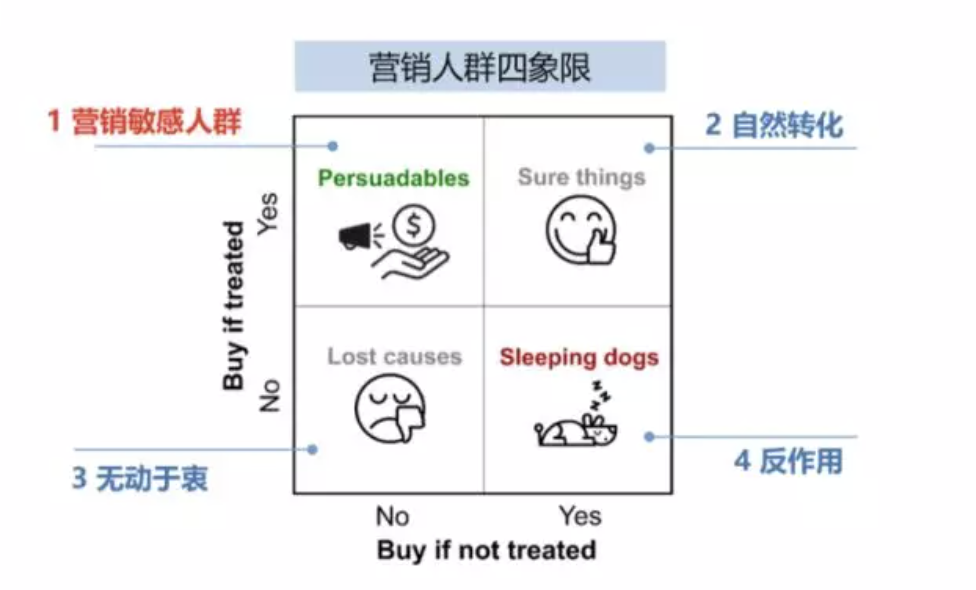
\includegraphics[width=.8\textwidth]{fig/CasualInference-Uplift-Model-Population.png}
\end{figure}

图表解读:
\begin{itemize}
\setlength{\itemsep}{0pt}
\setlength{\parsep}{0pt}
\setlength{\parskip}{0pt}
    \item 横坐标:左边-用户不被treat,不会购买;右边-用户不被treat,会购买;
    \item 纵坐标:上边-用户被treat,会购买;下边-用户被treat,不会购买;
    \item 所以有四象限的人群:
    \begin{itemize}
\setlength{\itemsep}{0pt}
\setlength{\parsep}{0pt}
\setlength{\parskip}{0pt}
    \item 左上:不treat时,不购买,treat 后,购买(营销敏感人群)
    \item 右上:不treat时,购买,treat 后,购买(自然转化)
    \item 左下:不treat时,不购买;treat 后,不购买(无动于衷)
    \item 右下:不treat时,购买;treat 后,不购买(反作用)
\end{itemize}
\end{itemize}

比如,我们对人群做四象限的划分,横纵坐标分别是用户在有干预和无干预情况下的购买状况。如上图,左上角人群的购买状况在干预后发生了正向变化,如果我们不对这类人群进行干预,那他有可能是不购买的,但是干预之后的购买概率有极大提升,所以这类人群是我们真正想要触达的用户,即\textbf{营销敏感人群}。而其他人群比如第2类和第3类,在干预前后的购买状况没有变化,所以预算花费可能是浪费。右下角是一类比较特殊的人群,虽然其在干预前后的状态有跳变,但这种跳变不是我们希望看到的,因为确实有一些人群对营销是反感的,所以对这类人群我们应该极力避免触达。Uplift Model正是为了识别我们想要的营销敏感人群。

但是在现实生活中我们却没有办法准确的判断一个人是属于哪种类型,因为我们不可能对同一个用户同时treat和no treat。但是借助统计和机器学习的知识,我们就可以得到\textbf{相似的用户大致会怎么反应}。这就是uplift模型的核心,每一个用户会得到一个位于-1到1的lift score,用于指导用户人群的选择。

因此整个问题可以表述为:
\begin{figure}[H]
    \centering
    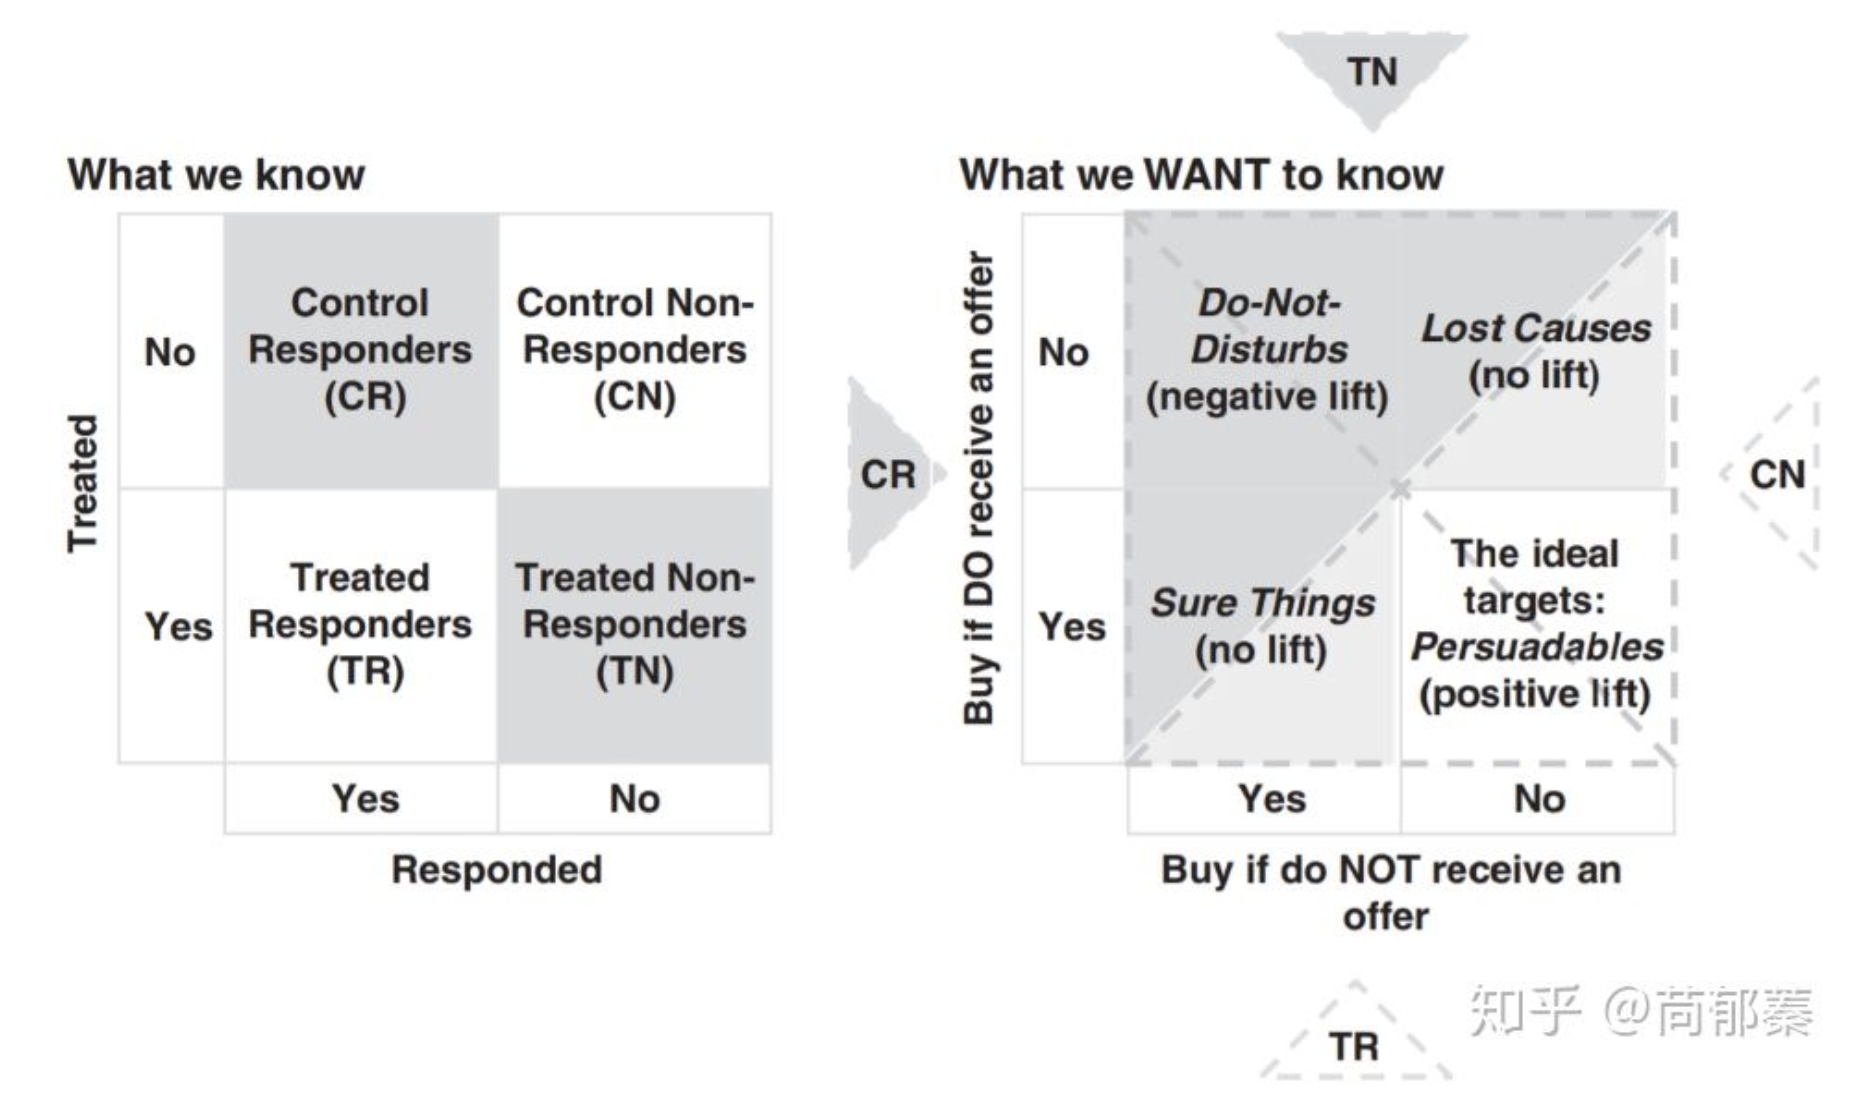
\includegraphics[width=1\textwidth]{fig/CasualInference-Uplift-Model-Problem.png}
\end{figure}

我们能获得的数据,是不同用户在treat或者no treat 下的 response(responder 或 non-responder);我们希望挖掘出来的是,用户如果不treat,是否buy;如果 treat,是否buy;

\section{Uplift Model的价值}
接下来介绍什么是Uplift Model,以及Uplift Model和传统的Response Model有什么样的差异。以广告投放为例,对于两个用户群,我们知道他们对广告投放的转化率分别是0.8\%和2\%,假如只有一次广告曝光的机会,应该向哪类用户投放广告?

按照以往的经验和直觉,可能会向第二类用户群投放广告,因为其转换率是最高的,但这个结论是对的吗?经过进一步分析,除了广告曝光转化率之外,,我们还能知道这两类用户群体在没有广告触达情况下的自然转化率(比如分别是:0.2\%和1.7\%),从而推算出广告所带来的增量。

比如第一类用户的广告转化率虽然低,但在没有广告触达情况下的转化率更低,即广告所带来的增量(uplift = 0.8\% - 0.2\% = 0.6\%)反而是比第二个用户更高的(uplift = 2\% - 1.7\% = 0.3\%),而我们要最大化总体的转化率其实等价于最大化广告的增量,按照这个逻辑,我们应该向第一个用户投放广告。也就是说Response Model很有可能会误导我们做出错误的决策,Uplift Model和Response Model之所以有差异,主要在于两个模型的预测目标不一样:
\begin{itemize}
\setlength{\itemsep}{0pt}
\setlength{\parsep}{0pt}
\setlength{\parskip}{0pt}
    \item Response Model:\textbf{看过}广告之后购买的概率,这本身是一个相关性(correlation,无法区分营销敏感人群和自然转化人群)
    \item Uplift Model:\textbf{因为}广告而购买的概率,这是一个因果推断的问题(causation,精准定位营销敏感人群)
\end{itemize}

\section{建模方法}
\subsection{形式化的定义}
$$
p(Y_i|X_i, T_i = 1) - p(Y_i|X_i, T_i = 0) 
$$
其中,$Y$为Potential Outcome,$X$为User Feature, $T$为Treatment indicator;

也就是说,$Y$代表结果 ( 比如用户的点击,转化等 ),$X$是用户维度的特征,$T$代表的是营销的变量 ( 1代表有干预,0代表无干预 )。

因此这个概率差值表示的是用户在有干预和没有干预情况下的变化,这个模型建模的难点在于我们获取到的训练数据是不完整的,对于个体来说,我们不可能同时观测到在有干预和没有干预两种情况下的表现,也就是因果推断中经常提到的\textbf{反事实}的问题。

\begin{framed}
进一步理解\cite{Uplift_Model_Principle_And_Practice}:

假设有 $N$ 个用户,$Y_i(1)$ 表示我们对用户$i$干预后的结果,比如给用户 $i$ 发放优惠券后(干预)用户下单(结果),$Y_i(0)$ 表示没有对用户干预的情况下用户的输出结果,比如没有给用户 $i$ 发放优惠券(干预),用户下单(结果)。用户 $i$ 的因果效应(causal effect)的计算方式就是:
$$
\tau_i = Y_i(1) - Y_i(0) \qquad \qquad (1) 
$$

\textbf{Uplift Model 的目标就是最大化$\tau_i$}。这是一个增量,即有干预策略相对于无干预策略的提升,简单讲就是干预前后结果的差值。

实际使用时会取所有用户的因果效应期望的估计值来衡量整个用户群的效果,称为\textbf{条件平均因果效应(Conditional Average Treatment Effect, CATE)}:
$$
CATE: \tau(X_i) = E[Y_i(1)|X_i] - E[Y_i(0)|X_i] \qquad \qquad (2)
$$

上式中 $X_i$ 是用户 $i$ 的特征,所谓的 conditional 指基于用户特征。

(2)式是理想的uplift计算形式,实际上,对用户$i$我们不可能同时观察到使用策略(treatment)和未使用策略(control)的输出结果,即不可能同时得到$Y_i(1)$和$Y_i(0)$。因为对某个用户,我们要么发优惠券,要么不发。将(2)式修改一下:
$$
Y_i^{obj} = W_iY_i(1) + (1-W_i)Y_i(0)
$$

其中$Y_i^{obs}​$是用户 $i$ 可以观察到的输出结果,$W_i$ 是一个二值变量,如果对用户 $i$ 使用了策略,$W_i = 1$,否则$W_i = 0$。

在条件独立的假设下,条件平均因果效应的期望估计值是:
$$
\tau(X_i) = E[Y_i^{obj}|X_i = x, W = 1] - E[Y_i^{obj}|X_i = x, W = 0] 
$$

上式要满足条件独立(CIA)的条件,即用户特征与干预策略是相互独立的:
$$
\{Y_i(1), Y_i(0)\} \bot W_i|X_i
$$

实践上,\textbf{满足CIA这样条件的样本的可以通过AB实验获取},因为时随机实验,可以保证用户(特征)与干预策略是相互独立的。

增益模型要优化 $\tau(X_i)$,值越高越好。然而一个用户不能同时观察到使用干预策略和不使用干预策略的结果,因此 $\tau(X_i)$ 是难以直接优化的。但如果通过AB实验,可以获得使用干预策略和不使用干预策略两组人群。因为通过A/B Test拆分流量得到的这两组样本在特征的分布上面是一致的。如果两组人群的特征分布一致,可以通过模拟两组人群的 $\tau(X_i)$ 得到个体用户的 $\tau(X_i)$。因此增益模型依赖AB实验的数据,\textbf{随机化实验是Uplift Model建模过程中非常重要的基础设施}。
\end{framed}

我们应当如何去建模呢?可以从人群的角度来对平均因果效应做统计,假设我们有两群\textbf{同质}用户,均来自一线城市/年龄段为25-35/女性,我们可以对其中一组用户进行广告投放,另外一组不进行任何干预,之后统计这两群人在转化率上的差值,这个差值可以被近似认为是具备同样特征的人可能的平均因果效应。所以Uplift Model本质是从训练样本中学习条件的平均因果效应,同时因为模型是具有一定的泛化能力,可以对没有见过的样本也进行预测。


\subsection{The transformed outcome tree}
Uplift models需要每一个人的两方面信息:是否给予treatment,产出label。理想情况下,我们可以得到一些个体在随机分配到实验组(treat group)和对照组(control group)后的数据,基于他们对于treatment的反应,outcome label可以被转化为下面这个矩阵(Athey and Imbens 2016)(实际情况中可以有其他的正负样本划分方法):
\begin{figure}[H]
    \centering
    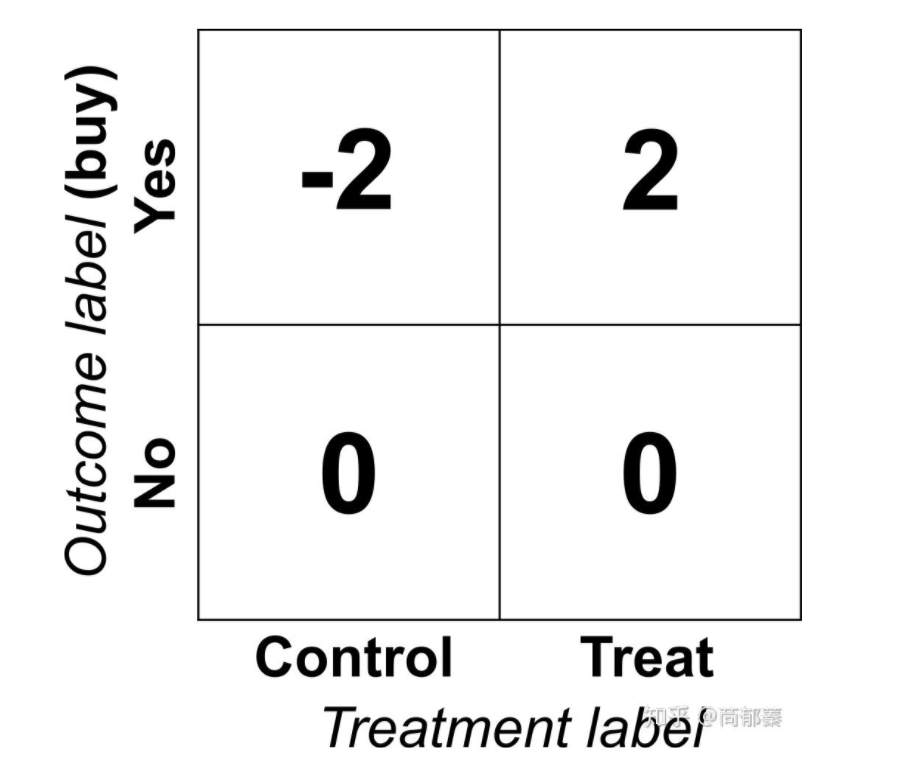
\includegraphics[width=.5\textwidth]{fig/CasualInference-Uplift-Model-Label.png}
\end{figure}

可能在第一眼的时候觉得这个目标矩阵不太靠谱,像拍脑袋的结果,为啥没有买的给不给treatment都是0?为什么给了treatment买了就是2?看起来非常不直观,但是是有道理在里面的,假如将一群人随机分为控制组和对照组,最后得到的平均值矩阵就是这群人的lift。

为了说明这个问题,考虑有一群人,人数为$2n$,其中$n$个给了treatment $t$,另外$n$个不给作为对照组。为了简单起见我们将$i =1 ,…, n$为treatment组$t$,$i =n+1 ,…, 2n$为控制对照组$c$。对于每一个用户,原始的outcomes和转换后的分别为 $y_i$ 和 $z_i$,那么对于这群人,对于购买行为的lift为:

\begin{align*}
Lift & = E[y|t] - E[y|c] \\
      & = \frac{1}{n}\sum_{i=1}^ny_i - \frac{1}{n}\sum_{i=n+1}^{2n}y_i \\
      & = \frac{1}{2n}[\sum_{i=1}^n2y_i - \sum_{i=n+1}^{2n}2y_i]  \\
      & = \frac{1}{2n}\sum_{i=1}^{2n}z_i \\
      & = E[z]
\end{align*}

也就是说,转化后的outcome取决于前一个group的lift,这个优雅的转换大大简化了lift问题,我们可以直接对$z$建立回归模型,我们就可以得到对于基于特征x表征的用户的uplift:
$$
\text{uplift}(x) = E[y|x,t] - E[y|x,c] = E[z|x]
$$


\subsection{建模方法}
\subsubsection{Two-Model(差分响应模型)}
最简单的Uplift建模方法是基于Two Model的差分响应模型,它的形式和前面介绍的Uplift Model的定义非常相似,包含了两个响应模型,其中\textbf{一个模型$G$用来估计用户在有干预情况下的响应},另外\textbf{一个模型$G'$是用来学习用户在没有干预情况下的响应}。也就是说,预测时时分别对实验组模型和对照组模型预测用户的分数,两个模型预测分数相减就得到了uplift score之后将两个模型的输出做差,就得到我们想要的uplift。

简单来说,就是\textbf{训练2个模型,首先圈定一个人群(同质人群),里面有被投放广告的,也有没有投放广告的},注意两个人群(投放广告与没有投放广告)的选取一定要有随机性。其中未投放广告的为对照组,投放广告的为实验组。\textbf{对两个人群分别建模,分别为model1和model2,当新来一个该圈定的同质人群流量,会分别输入到moedl1和model2分别得到p1和p2,p2-p1就是该用户流量的增益}\cite{Understand_Uplift_Model_In_Ads}。

这种建模方法的优点是比较简单容易理解,同时它可以套用我们常见的机器学习模型,如LR,GBDT,NN等,所以该模型的落地成本是比较低的,但是该模型最大的缺点是精度有限,这一方面是因为我们独立的构建了两个模型,这两个模型在打分上面的误差容易产生累积效应,第二是我们建模的目标其实是response而不是uplift,因此对uplift的识别能力比较有限。

\begin{figure}[H]
    \centering
    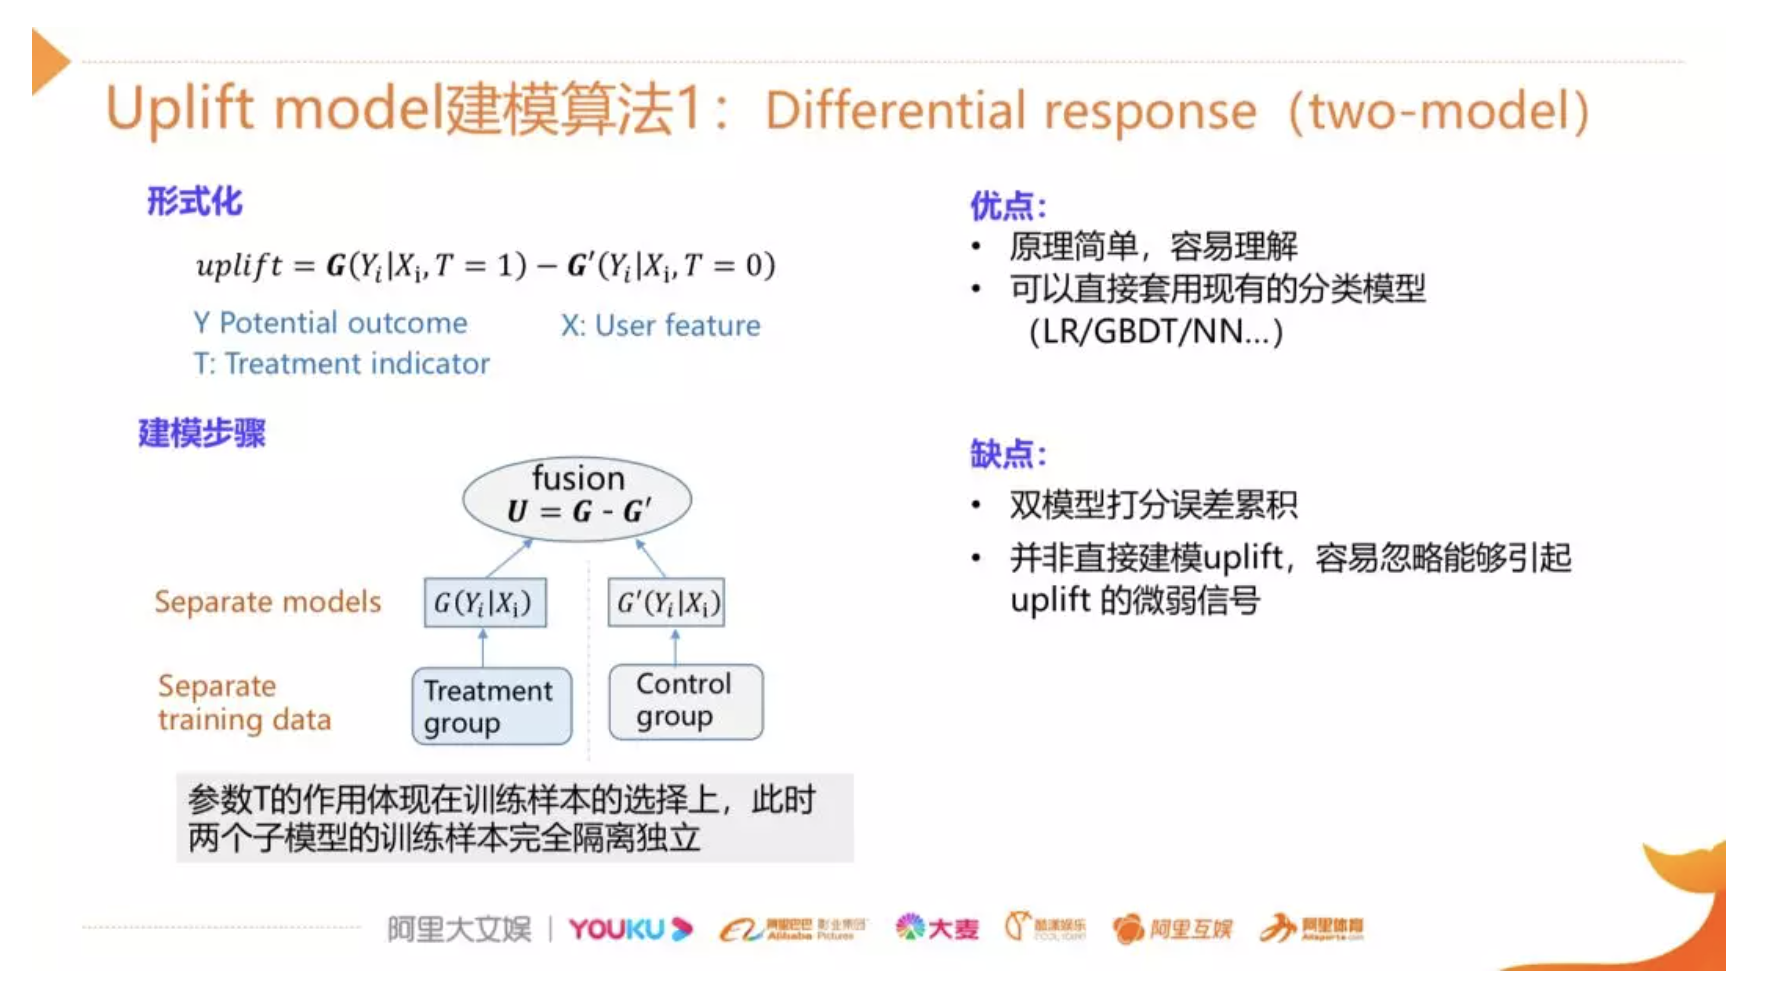
\includegraphics[width=1\textwidth]{fig/CasualInference-Uplift-Model-Two-Model.png}
\end{figure}

\begin{framed}
公式表述\cite{Uplift_Model_Principle_And_Practice}:

实验组是使用干预策略的用户(treatment),对照组是未使用干预策略的用户(control),正样本都是下单用户。即分别使用两个模型优化$E[Y_i^T|X_i^T]$和$E[Y_i^C|X_i^C]$,,得到两个模型,分别为:$G_T$和$G_C$。其中,$Y_i^T$和$X_i^T$分别是实验组用户 $i$ 的输出结果和特征;$Y_i^C$和$X_i^C$分别是控制组用户 $i$ 的输出结果和特征。

分别训练好两个模型之后,计算$E[Y^T|X^T] - E[Y^C|X^C]$就得到了条件平均因果效应分数。\textbf{这里因果效应分数是计算出来的而不是通过模型直接优化出来的,所以本质上,这还是传统的响应模型}。

以优惠券发放为例,目标是用户是否下单。训练时取实验组的用户训练,正样本是下单用户,负样本是未下单用户,预测结果是每个用户下单的概率。类似地,对照组也可以使用另一个模型预测出每个用户下单的概率。两个组的用户下单概率求平均,即可得到 $E[Y^T|X^T]$ 和 $E[Y^C|X^C]$,两者相减即得到 $\tau(X)$

预测时,对用户分别使用 $G_T$ 和 $G_C$ 预测,两个模型预测的分数相减即得到预测用户 $i$ 的 $\tau(X_i)$,最后根据 $\tau(X_i)$ 的高低决定是否发券。

\begin{figure}[H]
    \centering
    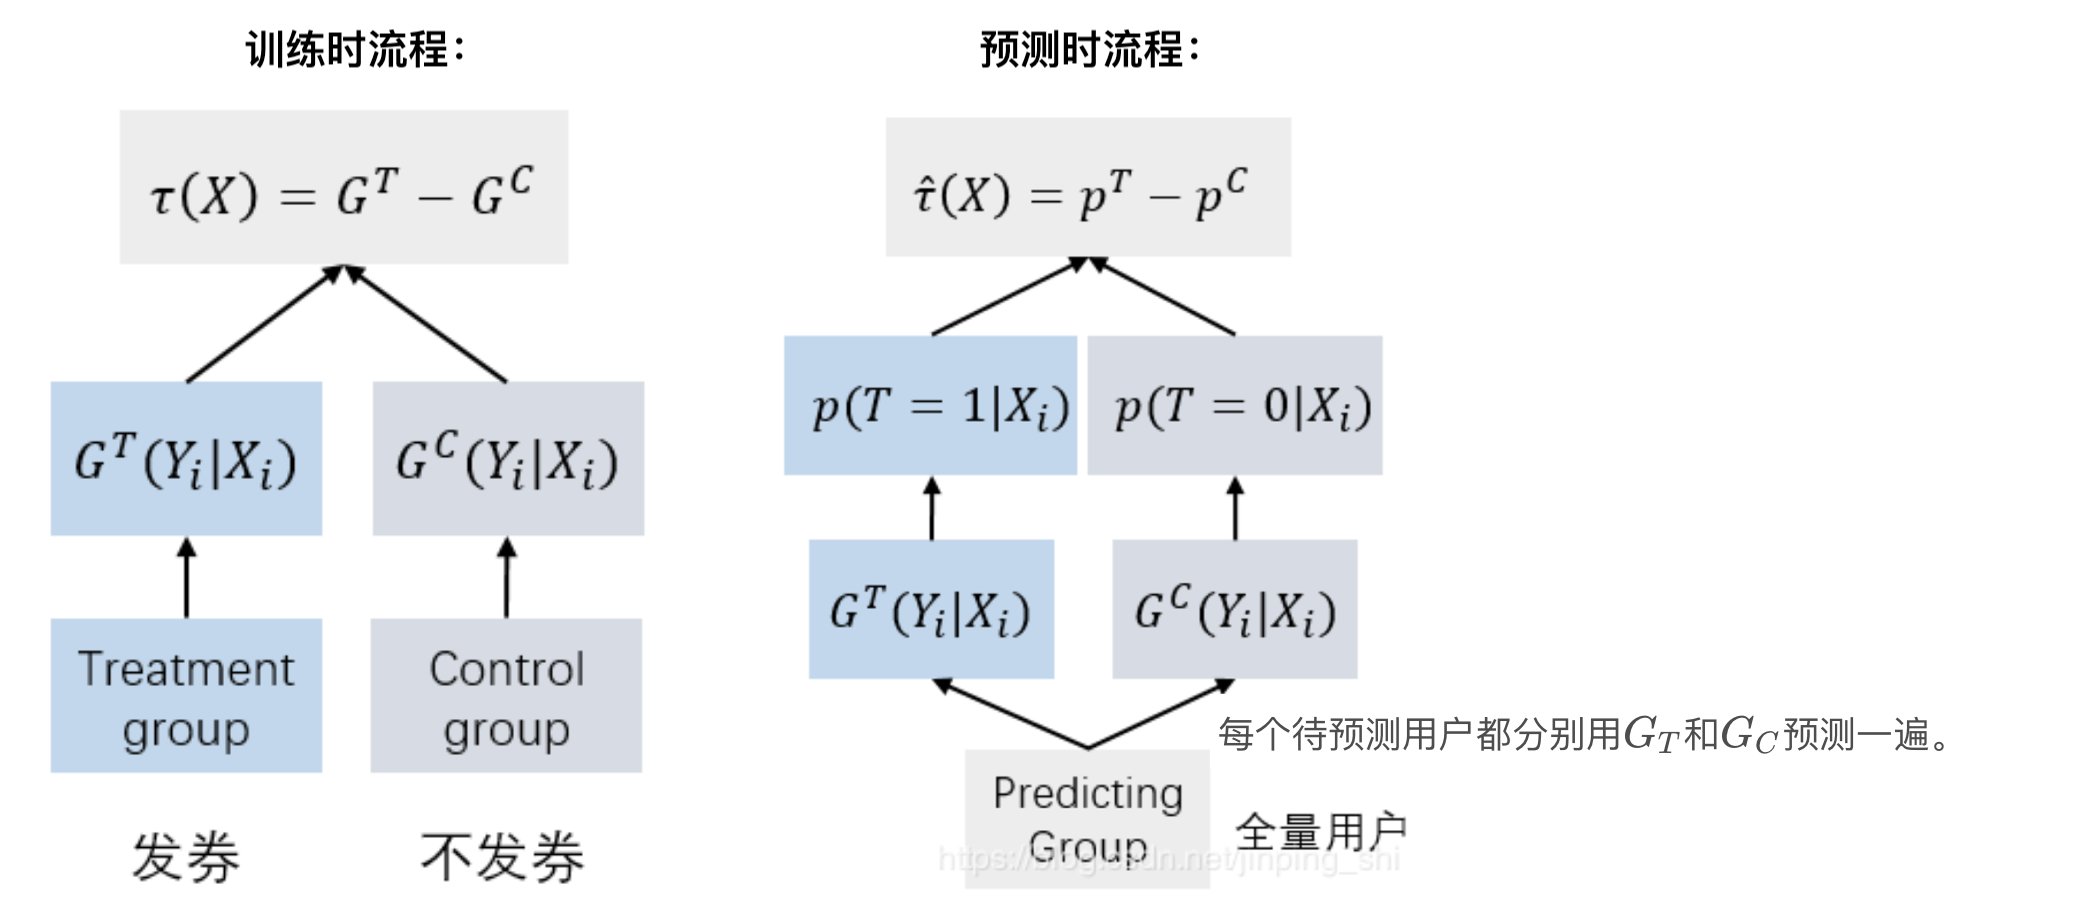
\includegraphics[width=1\textwidth]{fig/CasualInference-Two-Model-Train-Predict.png}
\end{figure}
\end{framed}

Two-Model 模型的优缺点:

差分响应模型简单粗暴,还很直觉。但只是模拟了 $\tau(X_i)$,没有真正优化 $\tau(X_i)$。两个独立的模型分开训练容易累积误差(两个独立模型的误差会累加传递到最终的 uplift score)。不过考虑到实现简单迅速,实践中可以作为baseline使用。

\subsubsection{One-Model(差分响应模型升级版)}
进一步地,还有一个基于One Model的差分响应模型,它和上一个模型最大差别点在于,它在模型层面做了打通,同时底层的样本也是共享的,之所以能实现这种模型层面的打通,是因为我们在样本的维度上做了一个扩展,除了user feature之外,还引入了与treatment相关的变量T ( T如果是0,1的取值可以建模single treatment,T也可以扩展为0到N,建模multiple treatment,比如不同红包的面额,或者不同广告的素材 ),One Model版本和Two Model版本相比最大的优点是训练样本的共享可以使模型学习的更加充分,同时通过模型的学习也可以有效的避免双模型打分误差累积的问题,另外一个优点是从模型的层面可以支持multiple treatment的建模,具有比较强的实用性。同时和Two Model版本类似,它的缺点依然是其在本质上还是在对response建模,因此对uplift的建模还是比较间接,有一定提升的空间,另外,这样是否还能够满足用户特征样与条件策略独立的假设是存疑的。

简单来说,同样首先圈定一个人群(同质人群),里面有被投放广告的,也有没有投放广告的,注意两个人群(投放广告与没有投放广告)的选取一定要有随机性。其中未投放广告的为对照组,投放广告的为实验组,\textbf{把是否被广告干预当作一个特征输入到模型中},然后与用户信息以及上下文信息一起训练一个模型model,\textbf{当新来一个该圈定的同质人群流量,会分别赋予该流量是否被广告干预特征T=0和T=1,和该广告流量对应的用户信息以及上下文信息一起输入到model中,得到p1和p2,p2-p1就是该用户流量的增益}。\cite{Understand_Uplift_Model_In_Ads}。

这里最重要的一点是,干预当成了了一个特征,这样会带来另外一个便利,T可以等于2,3,...(虽然都是广告投放,但是可以是不同的广告投放手段),那么就会给模型的创建带来更大的便利以解决更多的实际场景。

\begin{figure}[H]
    \centering
    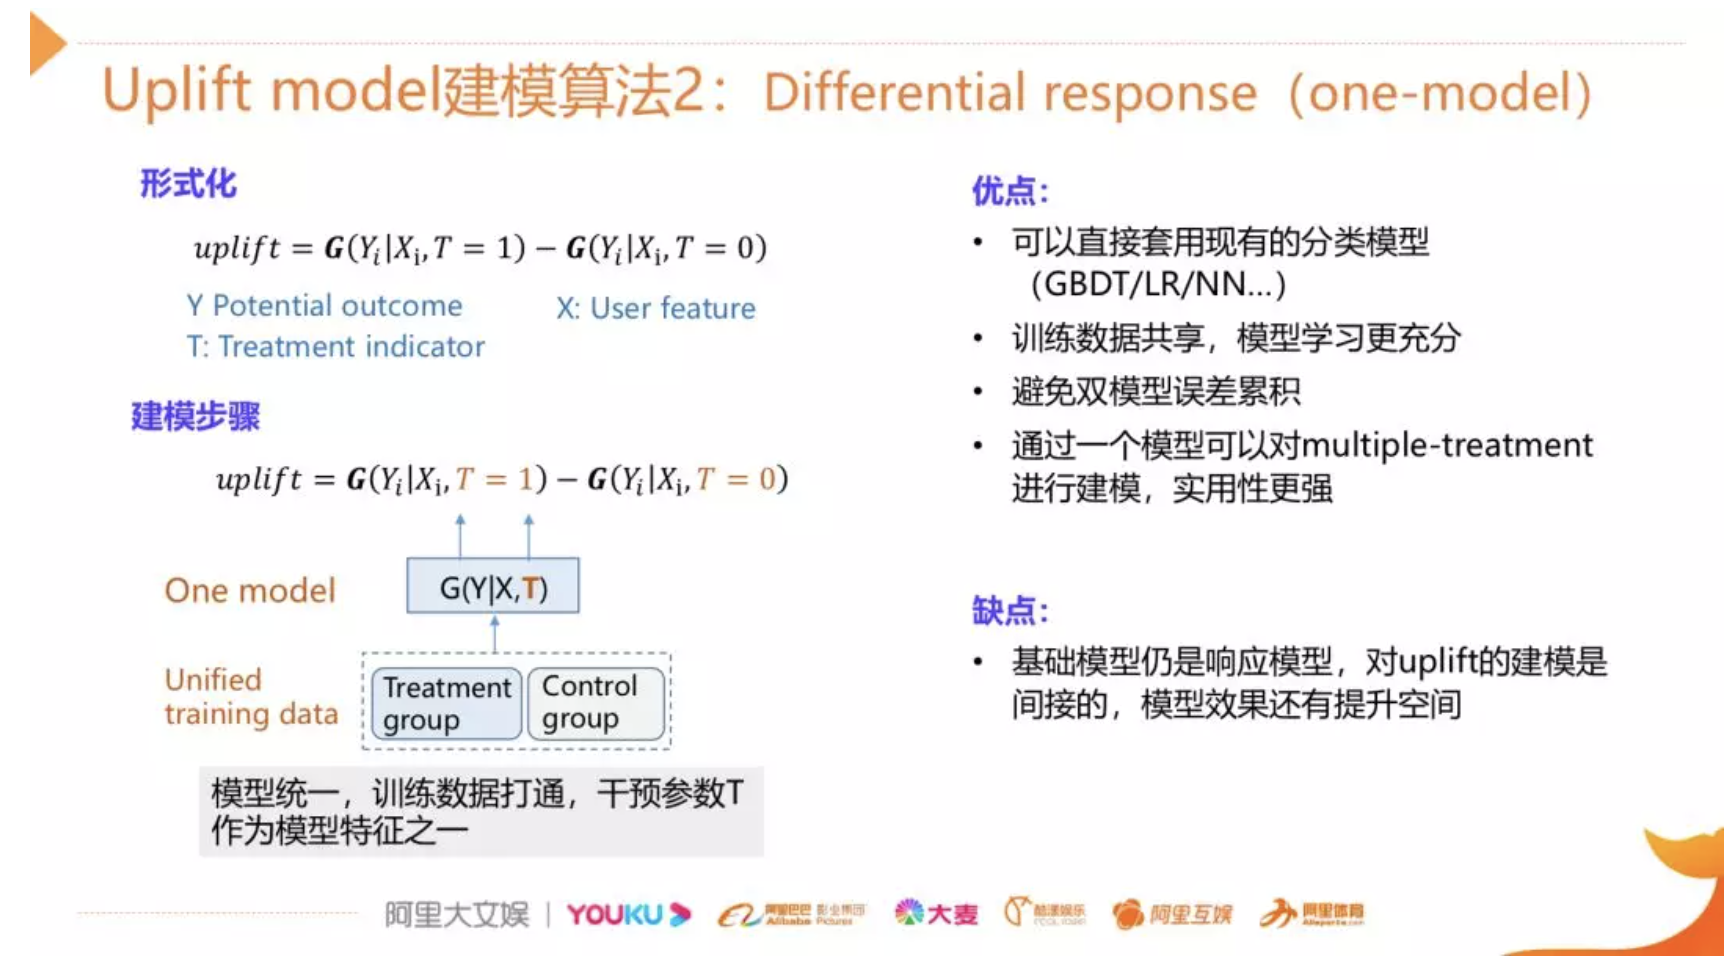
\includegraphics[width=1\textwidth]{fig/CasualInference-Uplift-Model-One-Model.png}
\end{figure}

\subsubsection{Class Transformation Method}
还有一种可以实现实验组对照组数据打通和模型打通的方法叫做class transformation method,可以直接优化 $\tau(X_i)$。

定义一个变量 $G = \{T, C\}$,$G = T$表示有干预,即实验组(treatment),$G = C$表示无干预,即对照组(control);uplift分数 $\tau$ 可以表示为:

\begin{align*}
\tau(X) &= P(Y = 1|X, G = T) - P(Y = 1|X, G = C) \\
	    &= P^T(Y = 1|X) - P^C(Y = 1|X) \qquad \qquad (5)
\end{align*}

上式中 $X$ 表示用户特征,$P^T$ \textbf{表示用户在实验组中下单的概率}(输出结果为positive),$P^C$ \textbf{表示用户在对照组中下单的概率}(输出结果也为positive),uplift score 就是两个概率的差值。

为了统一表示实验组和对照组都下单的情况($Y = 1$),再定义一个变量$Z, Z \in \{0, 1\}$:
$$
Z = \begin{cases}
1 \qquad \text{if} \ G = T \ \text{and} Y = 1 \\
1 \qquad \text{if} \ G = C \ \text{and} Y = 0 \\
0 \qquad \text{otherwise}
\end{cases}
$$

下面证明优化(5)式相当于优化$P (Z=1 | X)$。

假设干预策略 $G$ 与用户相互独立,即 $G$ 独立于 $X$:$P(G|X) = P(G)$,(5)式可以转写为:
\begin{align*}
P(Z = 1|X) &= P(Z=1|X, G=T) P(G = T|X) + P(Z=1|X, G = C)P(G=C|X) \\
	&= P(Y=1|X, G=T) P(G = T|X) + P(Y=0|X, G = C)P(G=C|X) \\
	&= P^T(Y = 1|X)P(G = T) + P^C(Y=0|X)P(G=C) \qquad \qquad (6)
\end{align*}

注意到 $P(G=T)$ 和 $P(G=C)$ 是可以通过AB实验控制的,在随机化实验中,\textbf{如果实验组和对照组的人数是相等的,那么 $P(G=T)=P(G=C)=1/2$,一个用户被分在实验组(有干预策略)和被分在对照组(无干预策略)的概率是相等的}。 在该假设下,(6)式可以改写为:
\begin{align*}
2P(Z=1|X) &= P^T(Y=1|X) + P^C(Y=0|X) \\
	&= P^T(Y=1|X) + 1 - P^C(Y=1|X) \qquad \qquad (7)
\end{align*}

由(7)式可得:
\begin{align*}
\tau(X) &= P^T(Y=1|X) - P^C(Y=1|X) \\
	&= 2P(Z=1|X) - 1 \qquad \qquad (8)
\end{align*}

(8)式就是要计算的uplift score,此时只有$Z$一个变量,可以直接对$Z=1$建模,相当于优化$P(Z=1|X)$,而不需要分别对实验组 $P^T$ 和对照组 $P^C$ 单独建模。而 $P(Z=1|X)$ 可以通过任何分类模型得到,所以这个方法称为Class Transformation Method。

实际上,$Z=1$就是实验组中下单的用户和对照组中未下单的用户,因此可以直接将实验组和对照组用户合并,使用一个模型建模,实现了数据层面和模型层面的打通。\textbf{预测时,模型预测的结果就是uplift score,这点与差分响应模型不同}。

\begin{figure}[H]
    \centering
    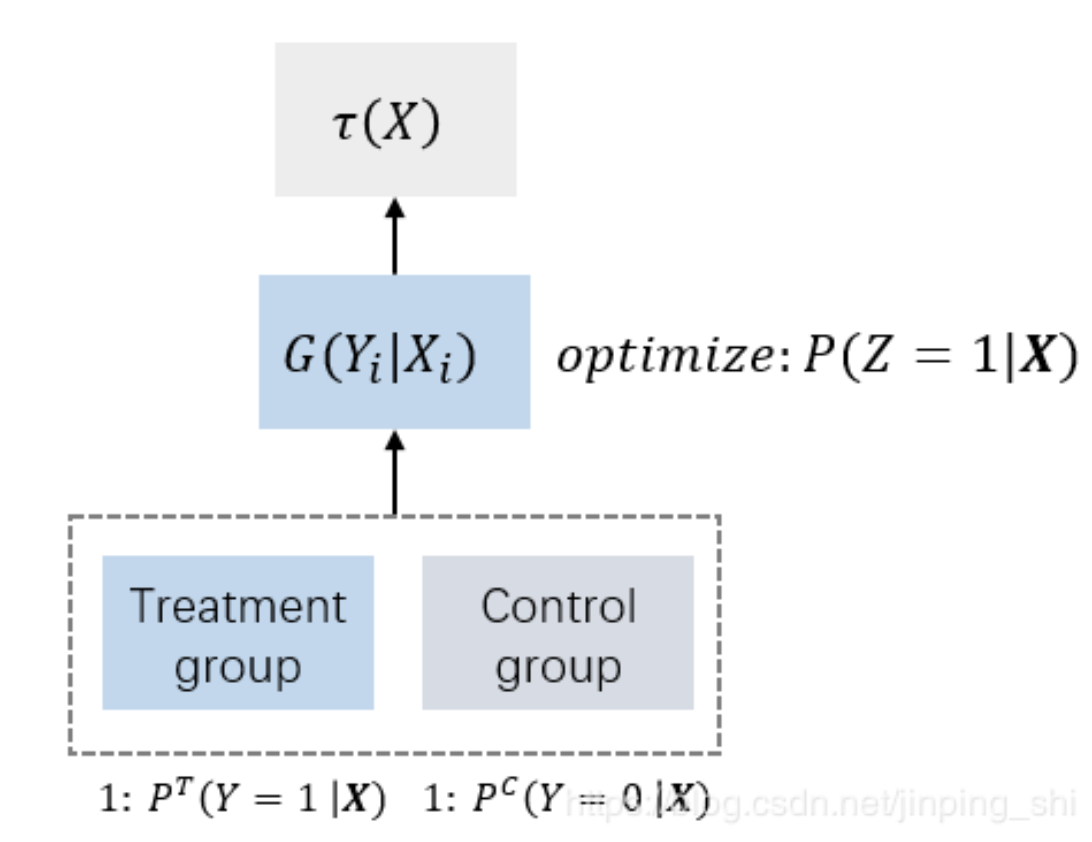
\includegraphics[width=0.6\textwidth]{fig/CasualInference-Uplift-Model-Class-Transformation.png}
\end{figure}

\begin{framed}
\textbf{Class Transformation的两个假设}

该方法有两个假设:
\begin{itemize}
\setlength{\itemsep}{0pt}
\setlength{\parsep}{0pt}
\setlength{\parskip}{0pt}
    \item $G$ 与 $X$ 相互独立;
    \item $P(G=T) = P(G = C) = \frac{1}{2}$
\end{itemize}

第一个假设很好理解,实践中保证用户特征与干预策略无关即可。第二个假设过于严格,难以在实践中每次都满足。但是可以通过\textbf{重采样}使得数据满足该假设,即使不满足(经常会有对照组数量远远小于实验组的情况),根据(6)式,训练数据的不平衡影响的只是 $P(G=T)$ 和 $P(G=C)$ 的权重(原来的权重是1:1),如果模型结果有意义,并且如果在测试集和线上表现良好,那么也不一定非要满足 $P(G=T) = P(G=C) = \frac{1}{2}$ 的假设,实践中都是结果导向。
\end{framed}

\subsubsection{Modeling Uplift Directly}
后续也有相关研究提出了直接的建模方法,通过对现有的模型内部进行深层次的改造来直接刻画uplift,其中研究较多的是基于树模型的uplift建模,下面主要介绍它的思想。

在传统的决策树构建中,最重要的环节是分裂特征的选择,我们常用的指标是信息增益或者信息增益比,其背后的含义还是希望通过特征分裂之后下游节点的正负样本的分布能够更加的悬殊,也就代表类的纯度变得更高。类似的,这种思想也可以引入到Uplift Model的建模过程中,虽然我们并没有用户个体的uplift直接的label,但是我们可以通过treatment组和control组转化率的差异来刻画这个uplift,以图中左下角的图为例,我们有T和C两组样本,绿色的样本代表正样本,红色的代表负样本,可以看到在分裂之前T和C两组正负样本的比例比较接近,但是经过一轮特征分裂之后,T和C组内正负样本的比例发生了较大的变化,左子树中T组全是正样本,C组全是负样本,右子树正好相反,C组的正样本居多,意味着左子树的uplift比右子树的uplift更高,即该特征能够很好的把uplift更高和更低的两群人做一个区分。如何从数学上度量这种概率分布的差异的方式呢?一些文章提出了可行的方法,比如基于KL散度,欧式距离,卡方距离的等等。这种模型的优点是可以直接对uplift进行建模,因此它的精度理论上是更高的,但是在应用层面我们需要做大量的改造和优化,除了前面介绍的分裂规则之外,我们还需要改造它的loss函数,后续的剪枝等一系列的过程,所以它的实现成本是比较高的。

也就是说\cite{Uplift_Model_Principle_And_Practice},该方法\textbf{直接修改树模型的特征分裂计算方法}。常用的特征分裂指标是信息增益(information gain):
$$
\Delta_{gain} = \text{info}_{\text{after}}(D) - \text{info}_{\text{before}}(D)
$$
,可以直接改为:
$$
\Delta_{gain} = D_{\text{after}}(P^T, P^C) - D_{\text{before}}(P^T, P^C)
$$
其中 $D_{\text{before}}(P^T, P^C)$ 和 $D_{\text{after}}(P^T, P^C)$ 分别是分裂前后treatment和control样本的分布,可以用KL散度(KL divergence)、欧氏距离或者卡方距离来刻画这样的分布。

该方法可以直接对uplift建模,理论上精度会很高,但实际应用上除了修改分裂规则外,还需修改loss函数、剪枝算法等,成本较高。

\begin{figure}[H]
    \centering
    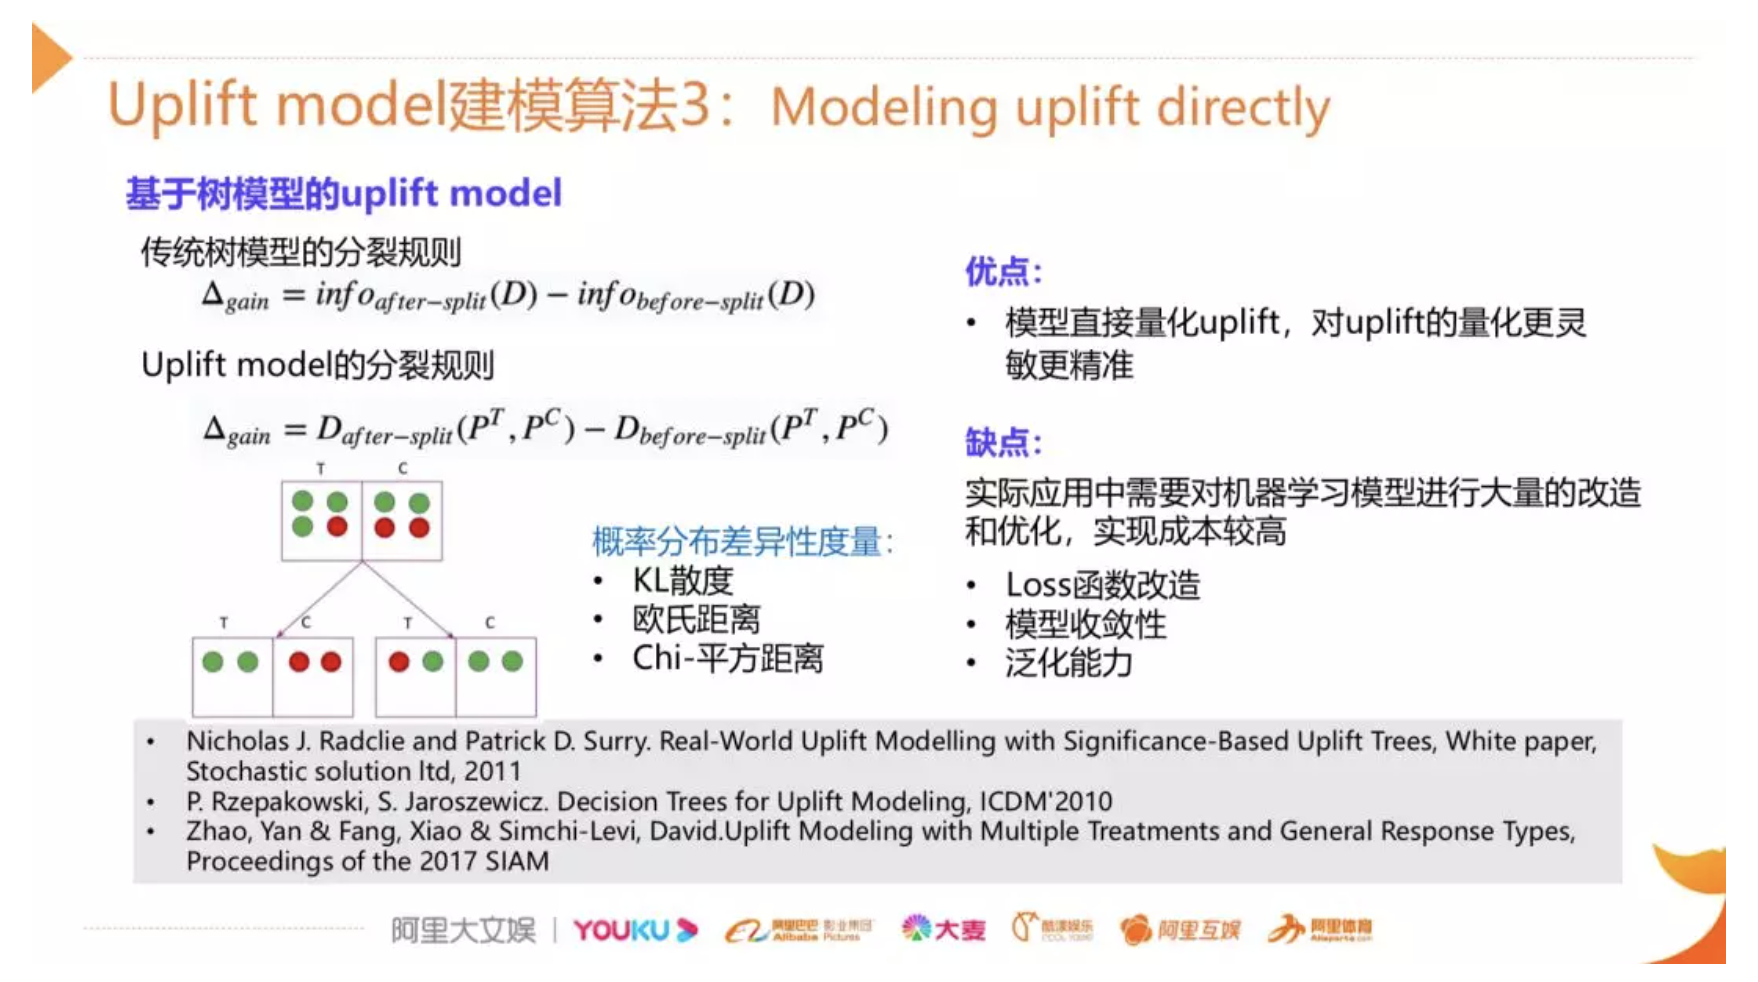
\includegraphics[width=1\textwidth]{fig/CasualInference-Uplift-Model-Direct-Model.png}
\end{figure}

\subsection{Evaluation metrics}
响应模型可以通过一个测试数据集来计算precision,recall和AUC,但是因为增益模型中不可能同时观察到同一用户在不同干预策略下的响应,所以uplift评估最大的难点在于我们并没有单个用户uplift的ground truth,传统的评估指标像AUC是无法直接使用的。

增益模型通常都是通过划分十分位数(decile)来对齐实验组和对照组数据,间接评估,而不是在一个测试集上直接评估。

\subsubsection{uplift 柱状图}
测试集上,实验组和对照组的用户分别按照uplift由高到低排序,划分为十等份,即十分位(decile),分别是top 10\%用户,top 20\%用户……top 100\%用户。分别对实验组和对照组中每个十分位内的用户求$E[Y^T|X^T]$和$E[Y^C|X^C]$,即预测分数的均值,然后相减,作为这个十分位bin内的uplift,绘制柱状图,如下图(这个图是由低到高排序,排序反了):
\begin{figure}[H]
    \centering
    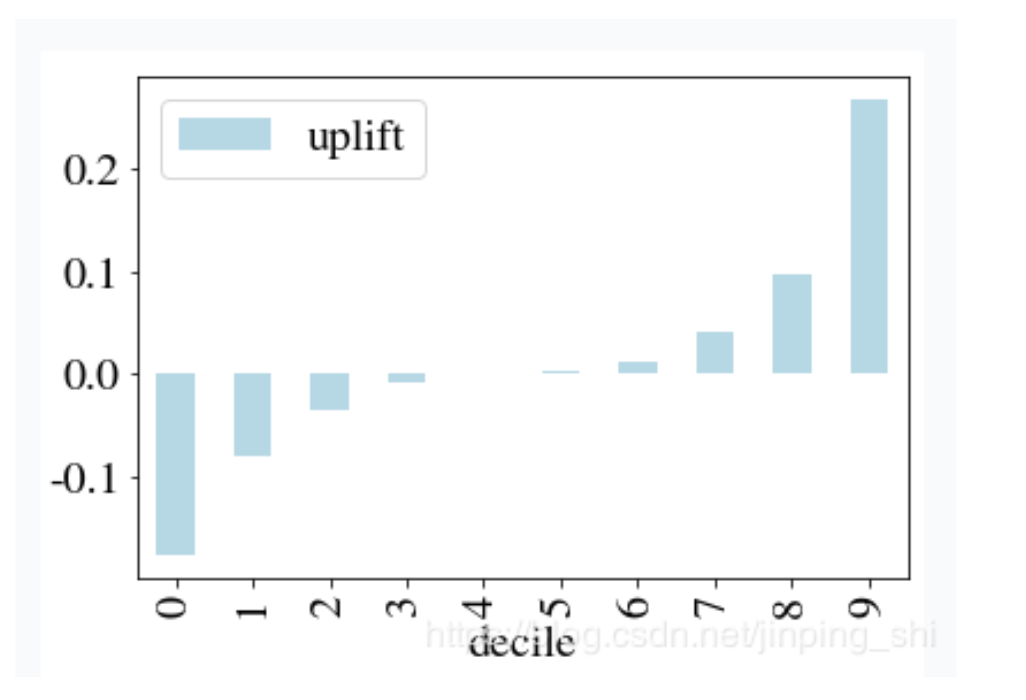
\includegraphics[width=.6\textwidth]{fig/CasualInference-Uplift_Evaluate_Bar.png}
\end{figure}
这种方法只能定性分析,无法计算出一个具体的值来整体评价模型的好坏。

\subsubsection{Qini指标和AUUC曲线}
我们下面再介绍一种评估指标,然后介绍如何将这个指标引入Transformed Outcome method。

最典型的评估指标是Qini curve。 在uplift bars的基础上绘制曲线,类似AUC来评价模型的表现,这条曲线称为Qini curve,计算每个百分比的Qini系数,最后将这些Qini系数连接起来,得到一条曲线。:
$$
Qini = \frac{n_{t,1}(\phi)}{N_t} - \frac{n_{c,1}(\phi)}{N_c}
$$

$n_{t,1}(\phi)$和$n_{c,1}(\phi)$分别代表着对照组和控制组中outcome为1的人数,分数$\phi$表示观察人群占目标人群的比值(也就是说,$\phi$ 是按照uplift score由高到低排序的用户数量占实验组或对照组用户数量的比例,如$ \phi = 0.1$,表示实验组或对照组中前10\%的用户),$N_t$ 和 $N_c$表示实验组和对照组的总人数(独立于$\phi$)。

如下图,横轴等于0.2时,对应的纵轴大概是0.0032(uplift score),表示当uplift score等于0.0032时,可以覆盖前20\%的用户数量,从图上看,这部分用户就是persuadable用户。
\begin{figure}[H]
    \centering
    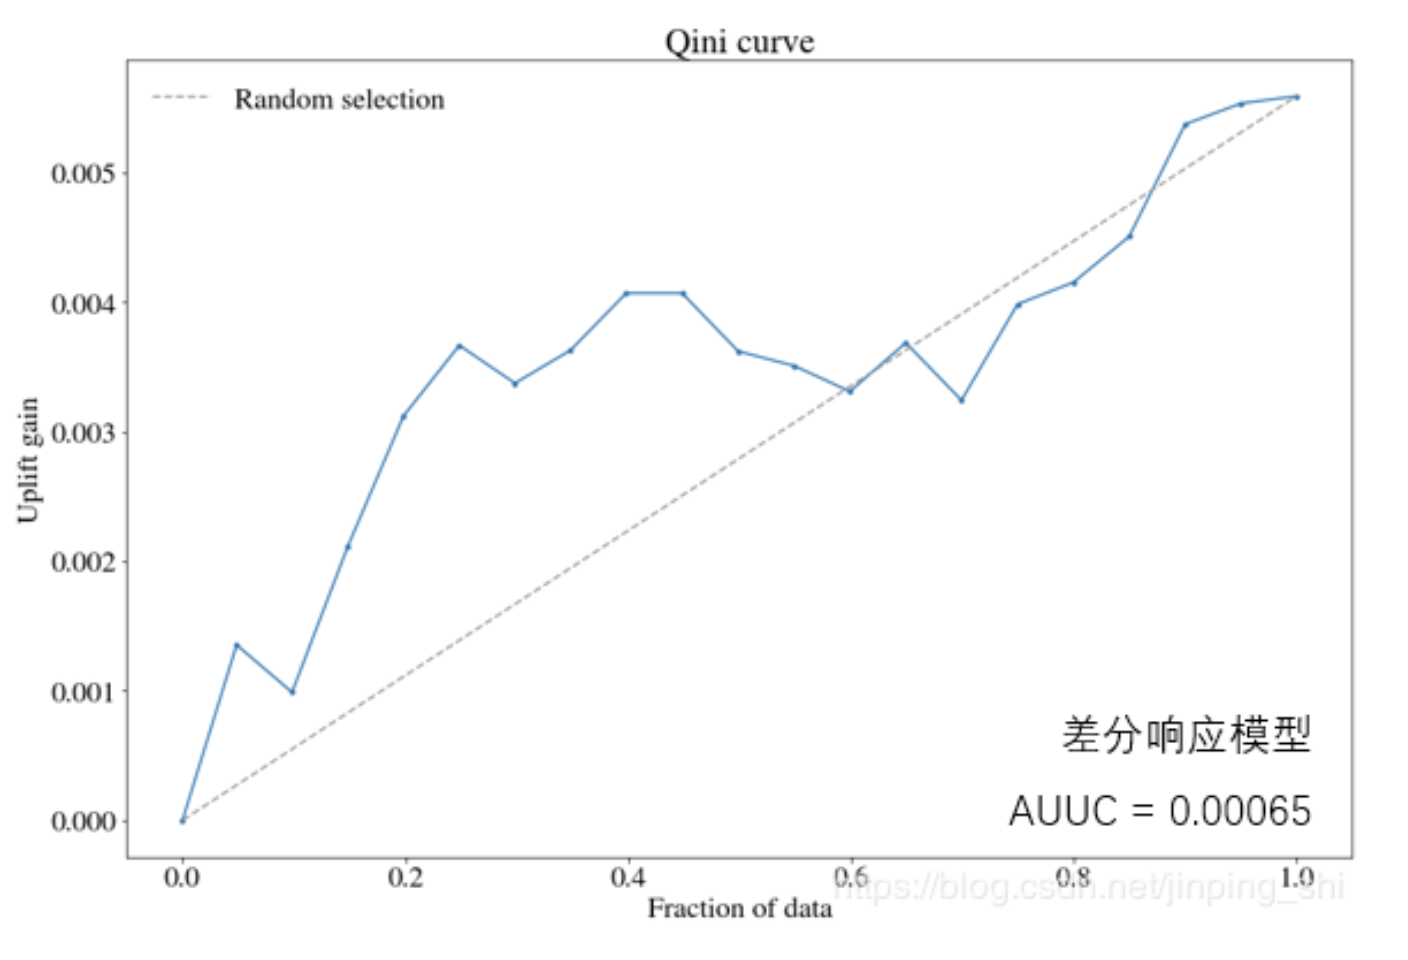
\includegraphics[width=.6\textwidth]{fig/CasualInference-Uplift_Evaluate_Qini_Curve.png}
\end{figure}

图中虚线是随机的base曲线,Qini曲线与随机random曲线之间的面积作为评价模型的指标,面积越大越好,面积越大,表示模型结果远超过随机选择的结果,与AUC类似,这个指标称为AUUC(Area Under Uplift Curve)。

\subsubsection{累积增益曲线(Cumulative Gain curve)}
因为$N_t$ 和 $N_c$其实并不独立于$\phi$,也就是实验组和对照组的均衡不是随机的,而是$\phi$的一个函数,所以Qini curve会自然的膨胀。为了纠正这一点,引入了以下两版曲线:
$$
G(\phi) =  (\frac{n_{t,1}(\phi)}{n_t(\phi)} - \frac{n_{c,1}(\phi)}{n_c(\phi)})(n_t(\phi) + n_c(\phi))
$$

各符号含义与Qini系数符号含义相同。其中 $n_t(\phi)$ 表示在 $\phi$ 百分比下,实验组(treatment)的用户数量,$n_c(\phi)$ 是在 $\phi$ 百分比下,对照组(control)的用户数量。与Qini系数相比,累积增益的分母是百分比 $\phi$ 下的实验组或对照组人数,并乘以 $n_t(\phi) + n_c(\phi)$ 作为全局调整系数,避免实验组和对照组用户数量不平衡导致的指标失真问题。

可以将累积增益曲线与random line之间的面积作为评价模型表现的指标。

\subsection{Uplift 总结}
增益模型实际上是一大类模型框架,本质上可以用传统响应模型或其他机器学习模型嵌入增益模型的框架,但是预测结果并不是一个概率,模型评价方式也有变化。

\subsubsection{训练样本收集}
增益模型建模强依赖于AB实验,数据要求很高。建模时要求实验组和对照组样本数量一样(实践中不一定有这个严格要求)。而且实验组和对照组的样本特征分布要一致,例如,训练数据不能是实验组预测后的结果、对照组随机选择的结果这样的组合,因为这样不满足干预策略与用户特征相互独立的假设($P(G | \boldsymbol{X}) = P(G$)。故实验组中还需要预留一部分随机选择的用户,与对照组中的用户作为模型迭代的数据,或者实验组与对照组都先经过某个策略或模型的筛选。

\subsubsection{多维度建模与个性化广告推送}
上述所有模型都是针对 $G=T$ 或者 $G=C$,即干预策略只有一种,对于发券,相当于一个treatment只有一种折扣,对于广告push,一个treatment也只能有一种内容。而treatment可以用多种维度,如不同渠道发放不同折扣的优惠券,不同场景推送不同内容的push。传统的response model以转化为多分类问题解决,但uplift modeling难以简单转化为多分类问题。

此外,个性化广告推送也依赖长期和短期的用户行为特征构建。不同营销场景下的用户特征可以共用,可以构建统一的线上线下特征平台。


\section{Python Uplift Modeling工具包:Pylift}
Pylift是uplift建模的Python工具包。Pylift在sklearn的基础上针对uplift modeling对各模型做了一些优化,同时集成了一套uplift评价指标体系。所以Pylift内核还是sklearn,在sklearn外面封装了一套API,针对树模型做了uplift优化,可以通过Pylift实现直接的uplift modeling.


\section{优惠券发放的 Demo}
\subsection{Demo 简介}
这里有一个优惠券发放的例子 。这是一次优惠券发放活动,对用户以短信方式发放5折优惠券,本次活动实验组(treatement,短信方式发送5折优惠券),对照组(不发券)37701名用户,注意到实验组和对照组不满足 $P(T) = P(C) = \frac{1}{2}$ 的条件。

这个例子还有一点特别,这其实是在\textbf{一个预测模型上再做一次uplift modeling}。本身实验组和对照组的数据是通过一个 XGB 模型预测出来的用户,该模型预测用户领取优惠券后是否会下单。根据模型预测结果,筛选一批高于某个阈值的用户,分成实验组和对照组。因此这次AB结果本身可以看出这个预测模型的uplift score。

这个预测模型的AB实验中,实验组转化率是2.69\%,对照组转化率是2.28\%,两组的转化率远高于以往运营随机筛选或根据条件筛选用户的转化率。但是,注意到这个预测模型的uplift score只有0.41\$(2.69\%-2.28\%)。说明预测模型筛选出来的用户本身就有下单意愿,并不一定是因为发放优惠券而下单,所以实验组中的用户 persuadable 的比例应该不是很高。

在一个预测模型上再做uplift modeling相当于是在下单意愿高的用户中再筛选persuadable用户,其实实践上没有太大必要。但是作为一个例子,数据还是比较完美的,而且实验组和对照都通过同一个预测模型筛选而来,然后再随机分组,是满足uplift modeling条件的。

\subsection{几种模型的示例}
\subsubsection{差分响应模型}
实验组和对照组分别建模,使用 lightGBM 模型,分别取80\%数据为训练集,20\%数据为测试集。两个模型在测试集上的表现如下(未调参):
\begin{figure}[H]
    \centering
    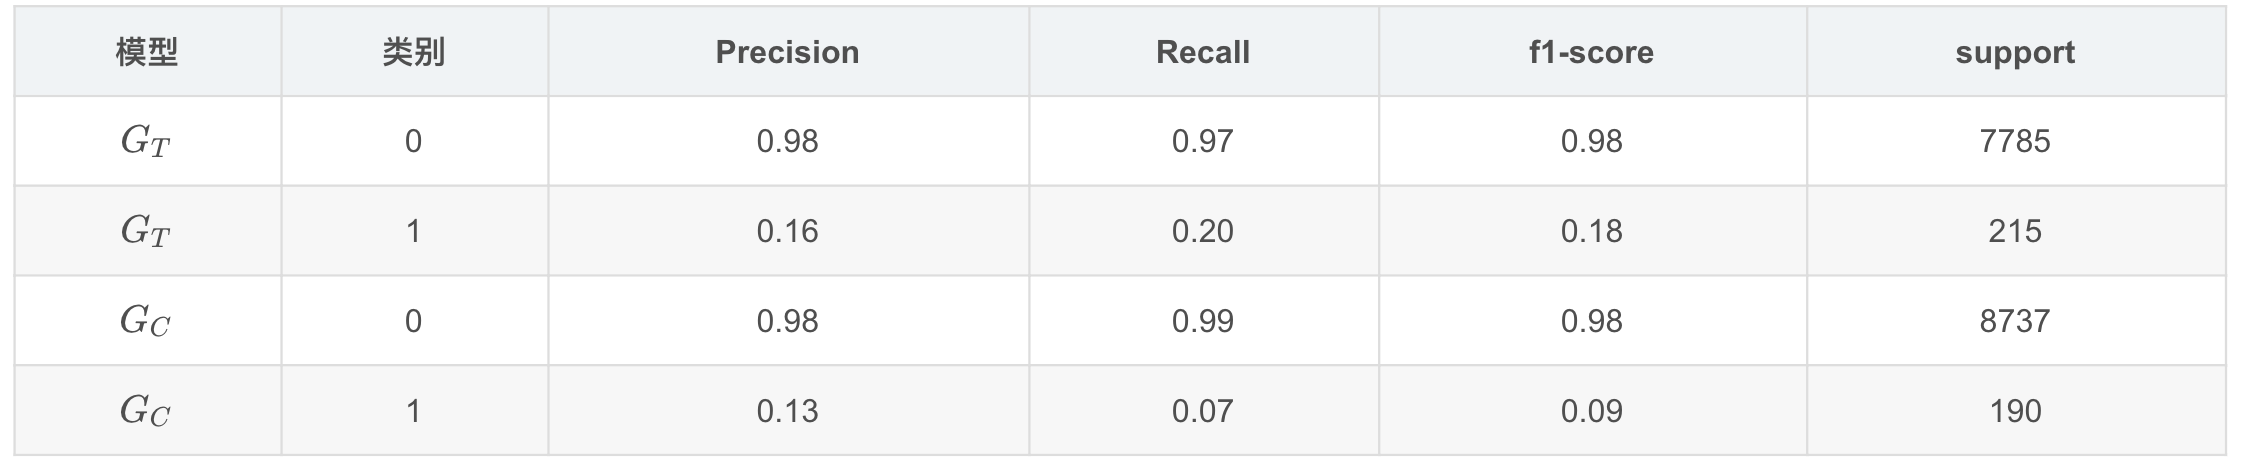
\includegraphics[width=1\textwidth]{fig/CasualInference-Uplift_Model_Demo_Table.png}
\end{figure}

方便起见,将实验组和对照组20\%的测试数据合并作为整个uplift model的测试集,流程如下。使用的数据集是经过了response model预测后的结果,相当于先筛选了一批下单概率高的用户,因为实验组和对照组用户都来自于同一个response model,可以认为两组用户特征分布式相同的。实际应用时,要注意实验组和对照组的用户特征分布是否一致。
\begin{figure}[H]
    \centering
    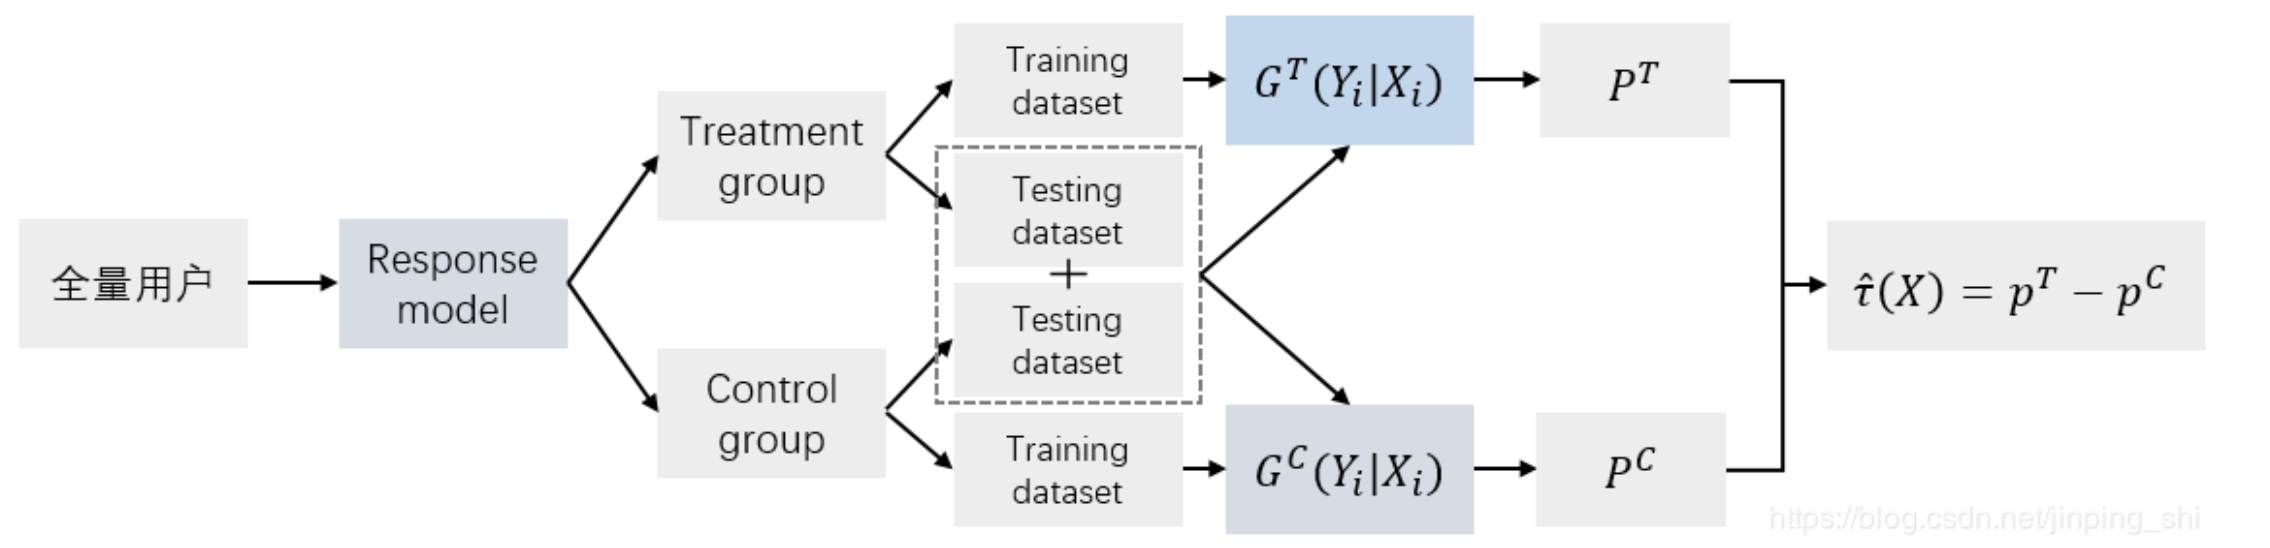
\includegraphics[width=1\textwidth]{fig/CasualInference-Uplift_Model_Demo2.png}
\end{figure}

对uplift分数 $\hat{\tau}(X)$ 排序,得到uplift bar,如下图所示。横轴是测试集中每个用户uplift的十分位数(decile),共10个bin;纵轴是每个bin的uplift均值。由于uplift排序是从低到高,因此这个uplift bar看起来是反的(正常应该是从高到底排)。
\begin{figure}[H]
    \centering
    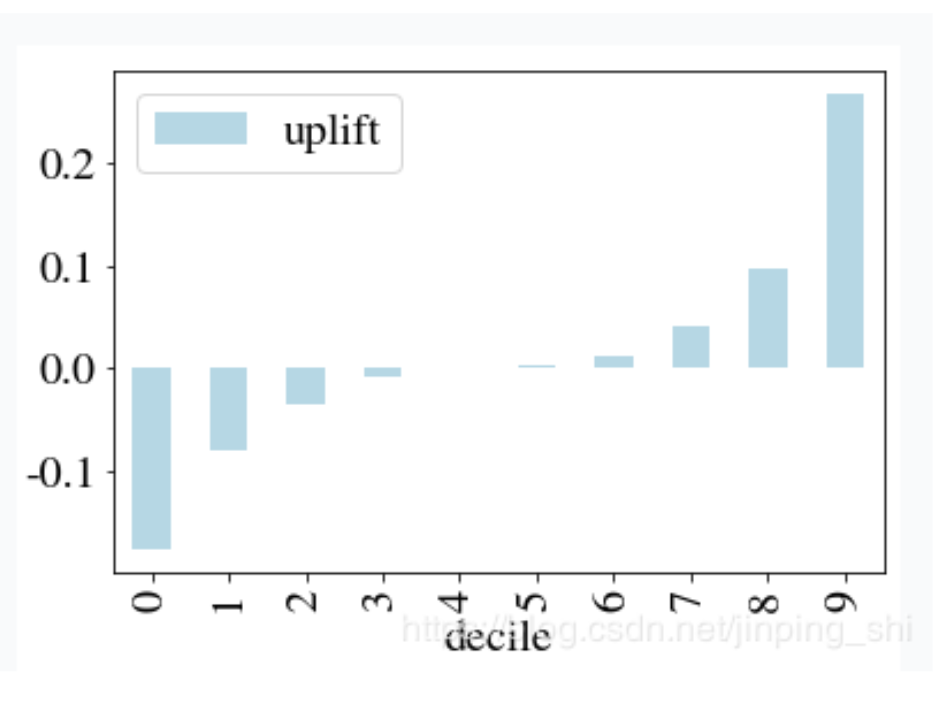
\includegraphics[width=.6\textwidth]{fig/CasualInference-Uplift_Model_Demo3.png}
\end{figure}

\subsubsection{Class Transformation Method}
训练和测试过程如下图所示。从实验组和对照组筛选出 $Z=1$ 的用户作为正样本,其余的作为负样本。同样使用lightGBM模型(未调参)。
\begin{figure}[H]
    \centering
    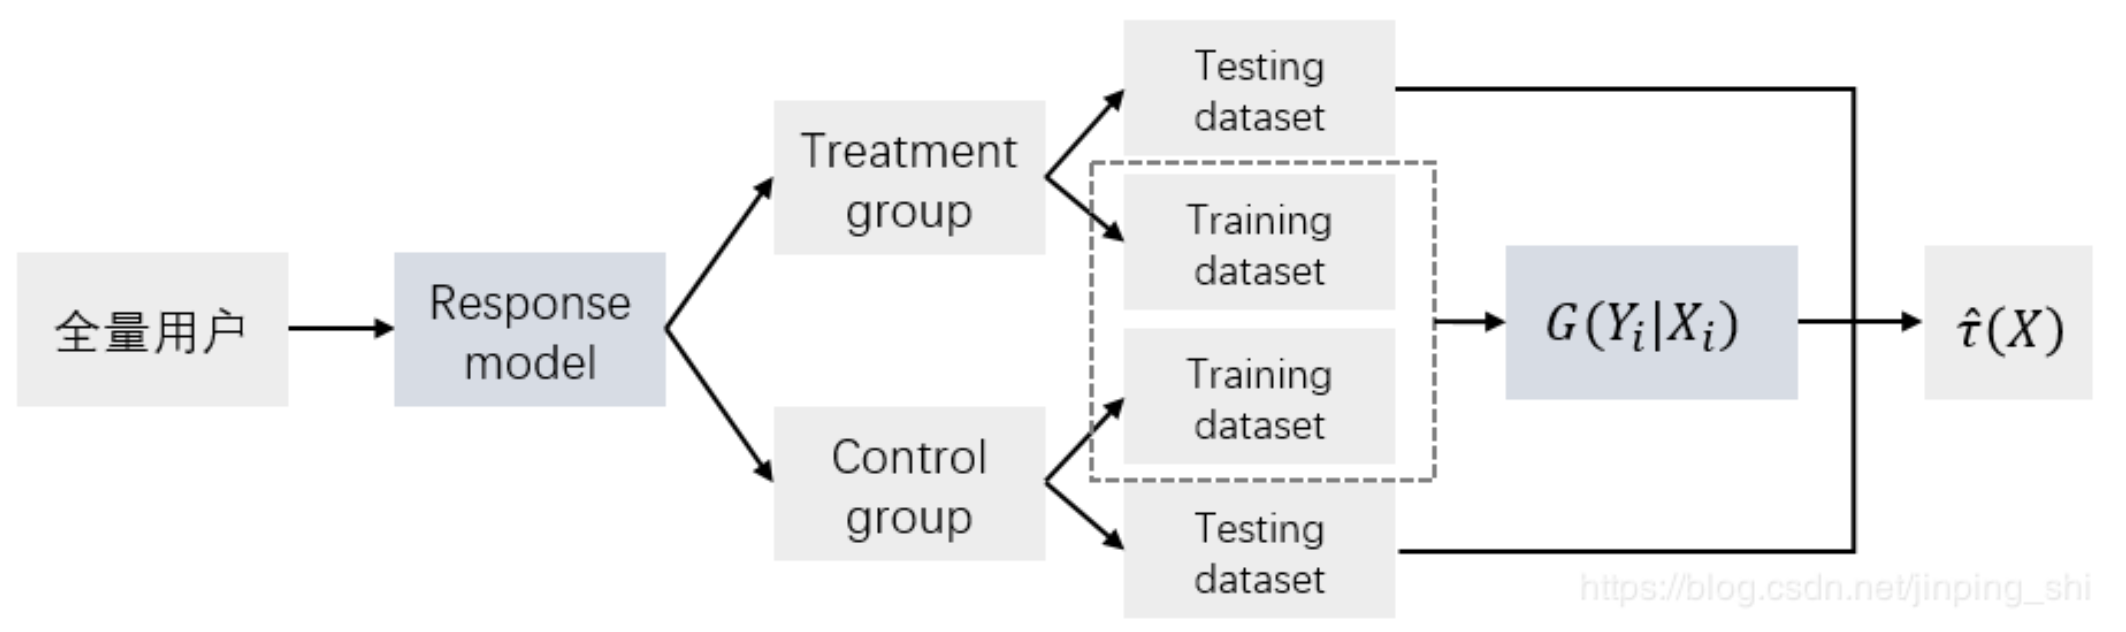
\includegraphics[width=1\textwidth]{fig/CasualInference-Uplift_Model_Demo4.png}
\end{figure}

\subsubsection{传统响应模型}
为了对比,这里生成了一份传统响应模型的结果。注意这个对比其实没有什么意义,因为这些数据本身就是一个响应模型预测的结果,再预测一次的意义不大。

响应模型使用LightGBM,正样本是下单用户,负样本是未下单用户,处理流程如下。将实验组(treatment group)切分为训练集和测试集,训练集用于训练预测模型,之后用该模型预测实验组的测试集作为 $P^T$,预测整个对照组的数据作为 $P^C$,然后计算uplift score。注意到这里实验组的测试集数量是远远少于对照组数量的,所以两边的数据量不均衡。这种方法计算出来的uplift score是模拟分数。
\begin{figure}[H]
    \centering
    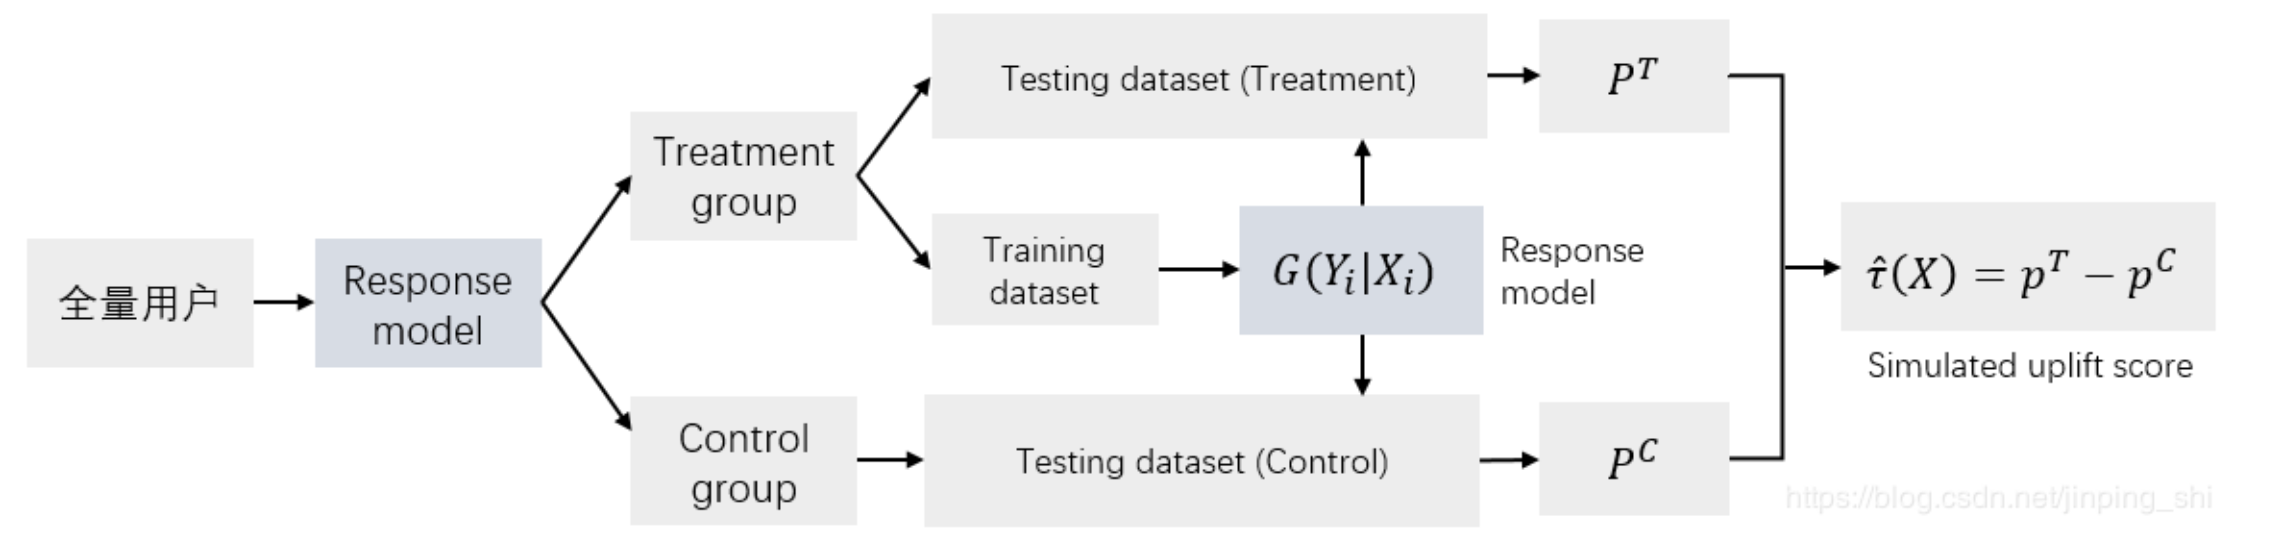
\includegraphics[width=1\textwidth]{fig/CasualInference-Uplift_Model_Demo5.png}
\end{figure}

\subsection{模型评估}
Qini曲线图如下。
\begin{figure}[H]
    \centering
    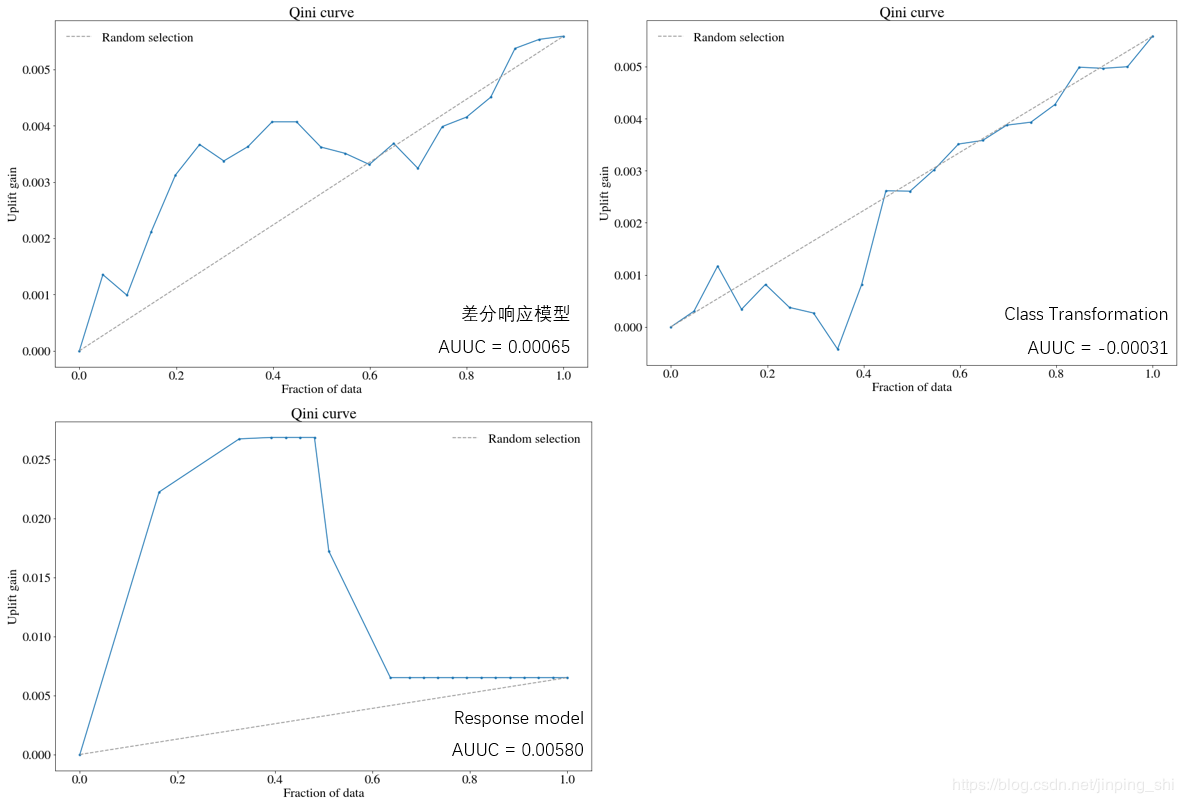
\includegraphics[width=1\textwidth]{fig/CasualInference-Uplift_Model_Demo6.png}
\end{figure}

Adjusted Qini是为了避免实验组和对照组数据不均衡而导致Qini系数失真而设计的。计算方式如下:
$$
AQini = \frac{n_{t,1}(\phi)}{N_t} - \frac{n_{c,1}(\phi)n_t(\phi)}{n_c(\phi)N_t}
$$

Adjusted Qini曲线如下:
\begin{figure}[H]
    \centering
    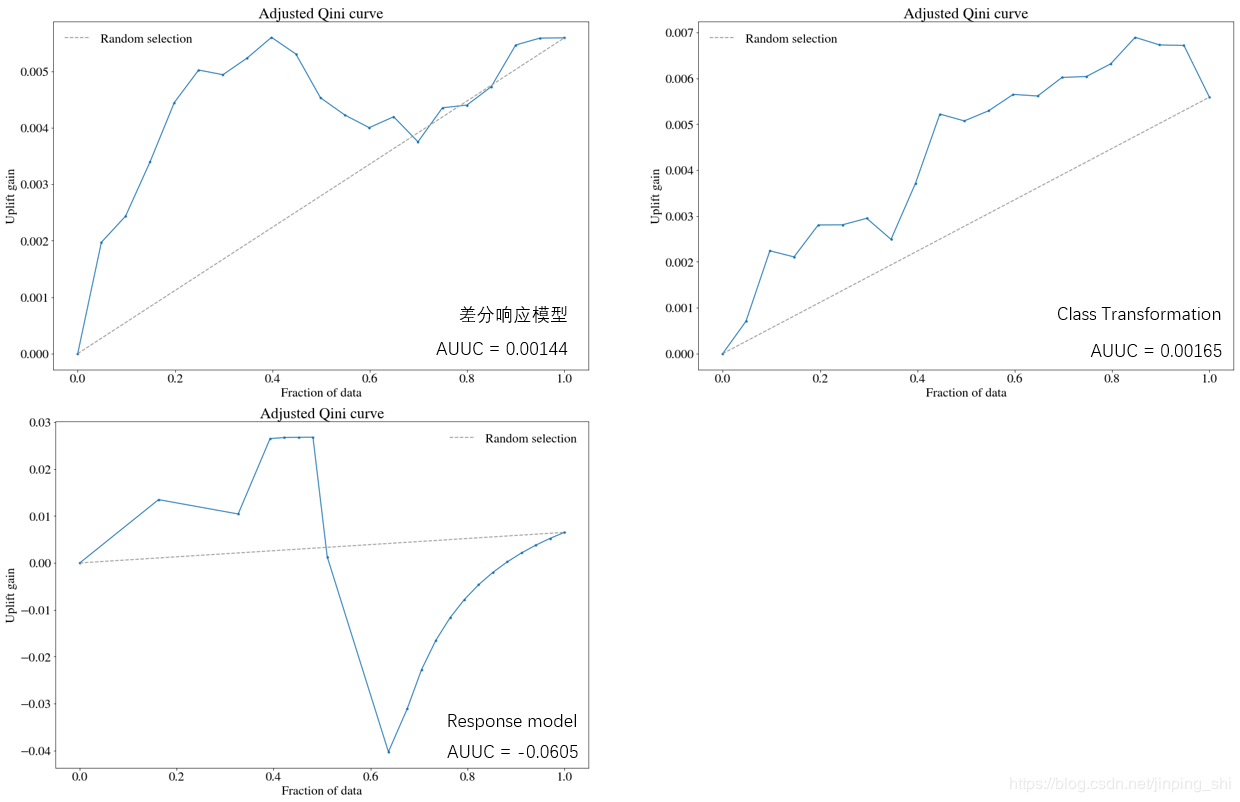
\includegraphics[width=1\textwidth]{fig/CasualInference-Uplift_Model_Demo7.png}
\end{figure}

累积增益曲线如下:
\begin{figure}[H]
    \centering
    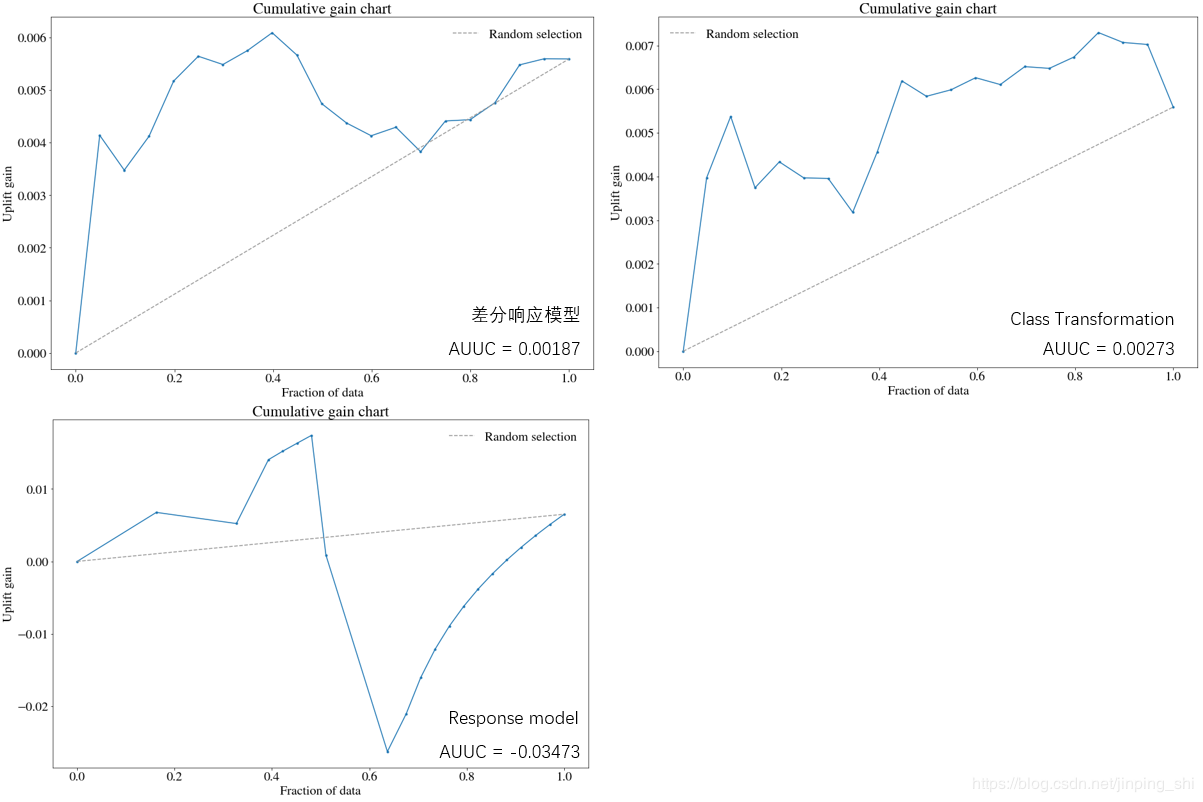
\includegraphics[width=1\textwidth]{fig/CasualInference-Uplift_Model_Demo8.png}
\end{figure}

在Qini曲线下,差分响应模型的总体效果要好一些。而在累积增益曲线下,Class Transformation模型的总体效果要好一些。实验组和对照组数据不平衡的情况下,Qini系数可能有偏差,但本次对比的实验数据两组用户数量是接近的,这个问题还在研究中。


\section{Uplift Model在淘票票智能票补中的应用}
下面以淘票票实际场景为例,来说明uplift model如何在实际场景中进行应用。该项目的目标是希望对进入到首页的用户个性化地发送红包,实现在预算和ROI的双重约束下提升平台总体购票转化率。我们的权益就是首页的红包,红包的使用规则、红包类型、预算和交互样式由产品运营设计,算法的作用是实现人和权益的精准匹配,我们需要确定应该给哪些用户发放以及发放哪种类型的权益。
\begin{figure}[H]
    \centering
    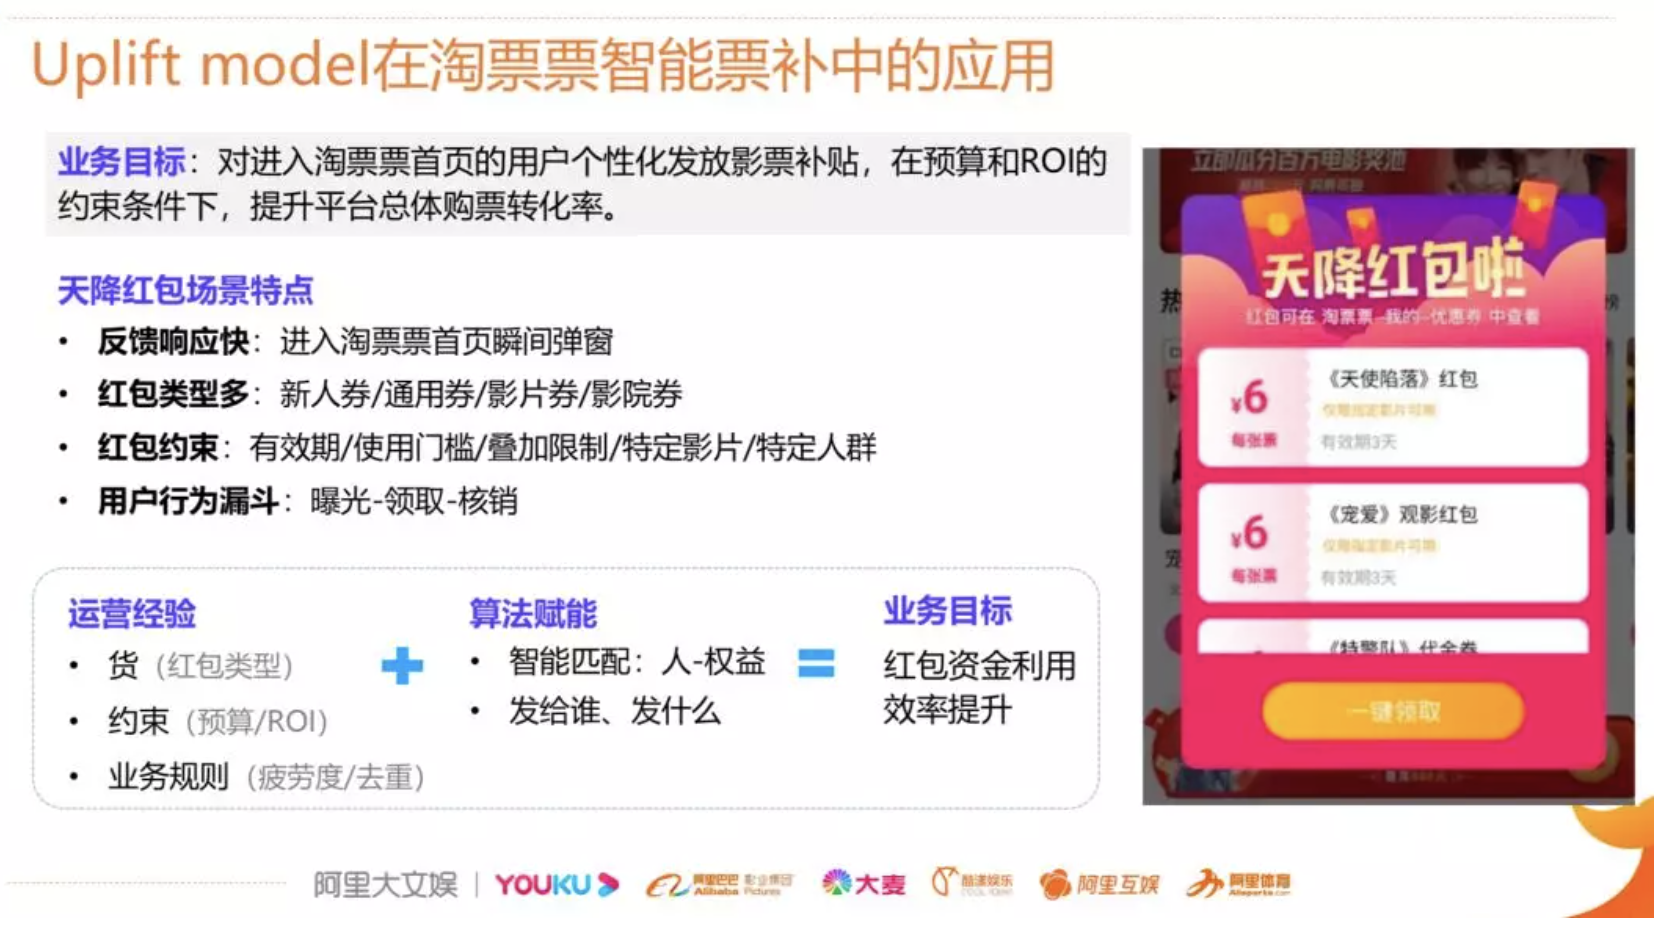
\includegraphics[width=1\textwidth]{fig/CasualInference-Uplift-Model-In-Ali.png}
\end{figure}

我们以平台通用券为例来说明问题是如何抽象和形式化的。在该场景下,每个用户最多只能发放一个红包,同时面额有固定几个分档,因此问题就精细化到如何对用户进行个性化的面额发放上,这可以通过经典的背包问题来抽象,如图所示,第一个公式是我们的目标,\textcolor{red}{最大化的是红包撬动效率,下面的约束条件一个是ROI约束,一个是预算约束}。目标函数公式中标红的部分是第$i$个用户在第$k$个红包下转化的uplift,$X_{ik}$是是否对用户$i$发放第$k$个红包,因此我们最终要决策的变量就是$X$矩阵。
\begin{figure}[H]
    \centering
    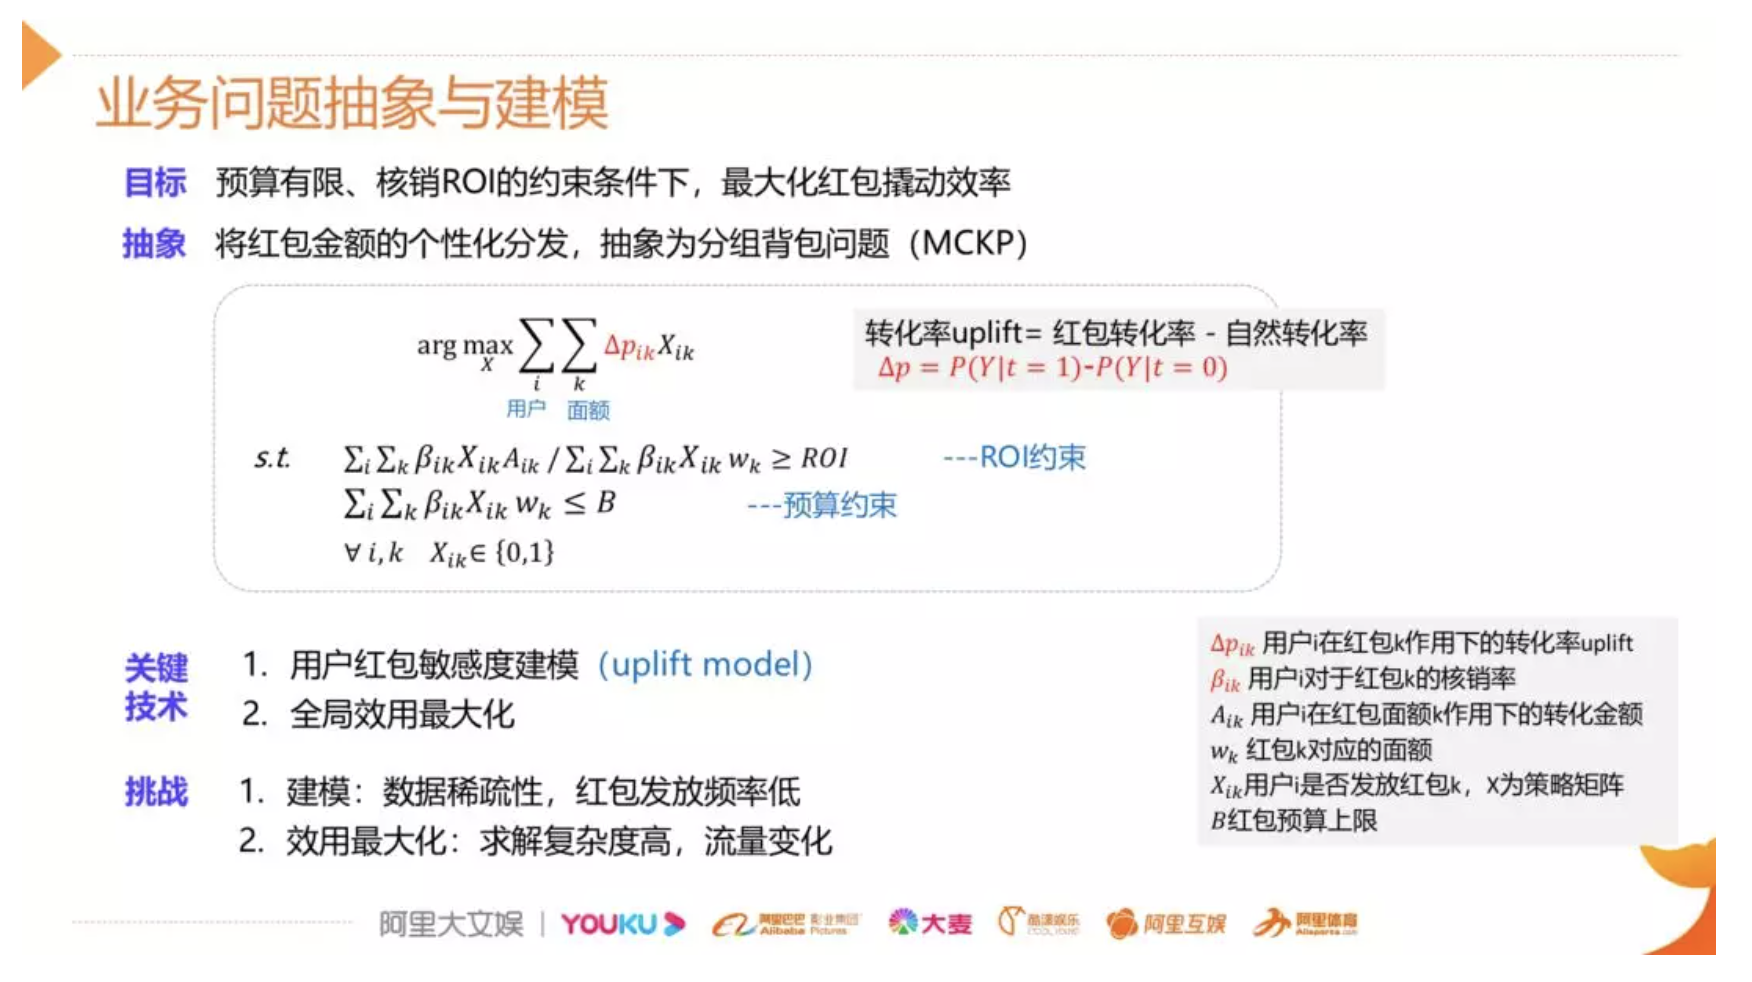
\includegraphics[width=1\textwidth]{fig/CasualInference-Uplift-Model-In-Ali2.png}
\end{figure}

\begin{align*}
\text{优化目标}: \qquad & \arg\max_x \sum_i\sum_k \Delta p_{ik}X_{ik}  \qquad(\text{其中,i代表用户维度,k代表券维度}) \\
\text{ROI 约束条件} \qquad & \sum_i\sum_k\beta_{ik}X_{ik}A_{ik} / \sum_i\sum_k\beta_{ik}X_{ik}w_k \ge ROI \\
\text{预算约束条件} \qquad & \sum_i\sum_k\beta_{ik}X_{ik}w_{k} \le B \\
& \forall i, k X_{ik} \in \{0, 1\}
\end{align*}

其中,转化率 uplift = 红包转化率 - 自然转化率,即$\Delta p = p(Y|t = 1) - P(Y|t = 0) $,即$\Delta p_{ik}$代表用户$i$在红包$k$下的转化率 uplift;

$\beta_{ik}$代表用户$i$对红包$k$的核销率;

$A_{ik}$代表用户$i$在红包面额$k$作用下的转化金额;

$w_{k}$代表红包$k$对应的面额;

$X_{ik}$代表是否对用户$i$发放红包$k$,$X$为策略矩阵;

$B$为红包预算上限;




该问题的求解中有两个关键点,一个是用户红包敏感度的建模,第二是在敏感度已知的情况下怎么进行全局效用最大化的求解。下面重点介绍uplift model模块。Uplift model的目标是预测每个用户在不同的红包金额下的转化率,从而构建出千人千面的敏感度曲线。
\begin{figure}[H]
    \centering
    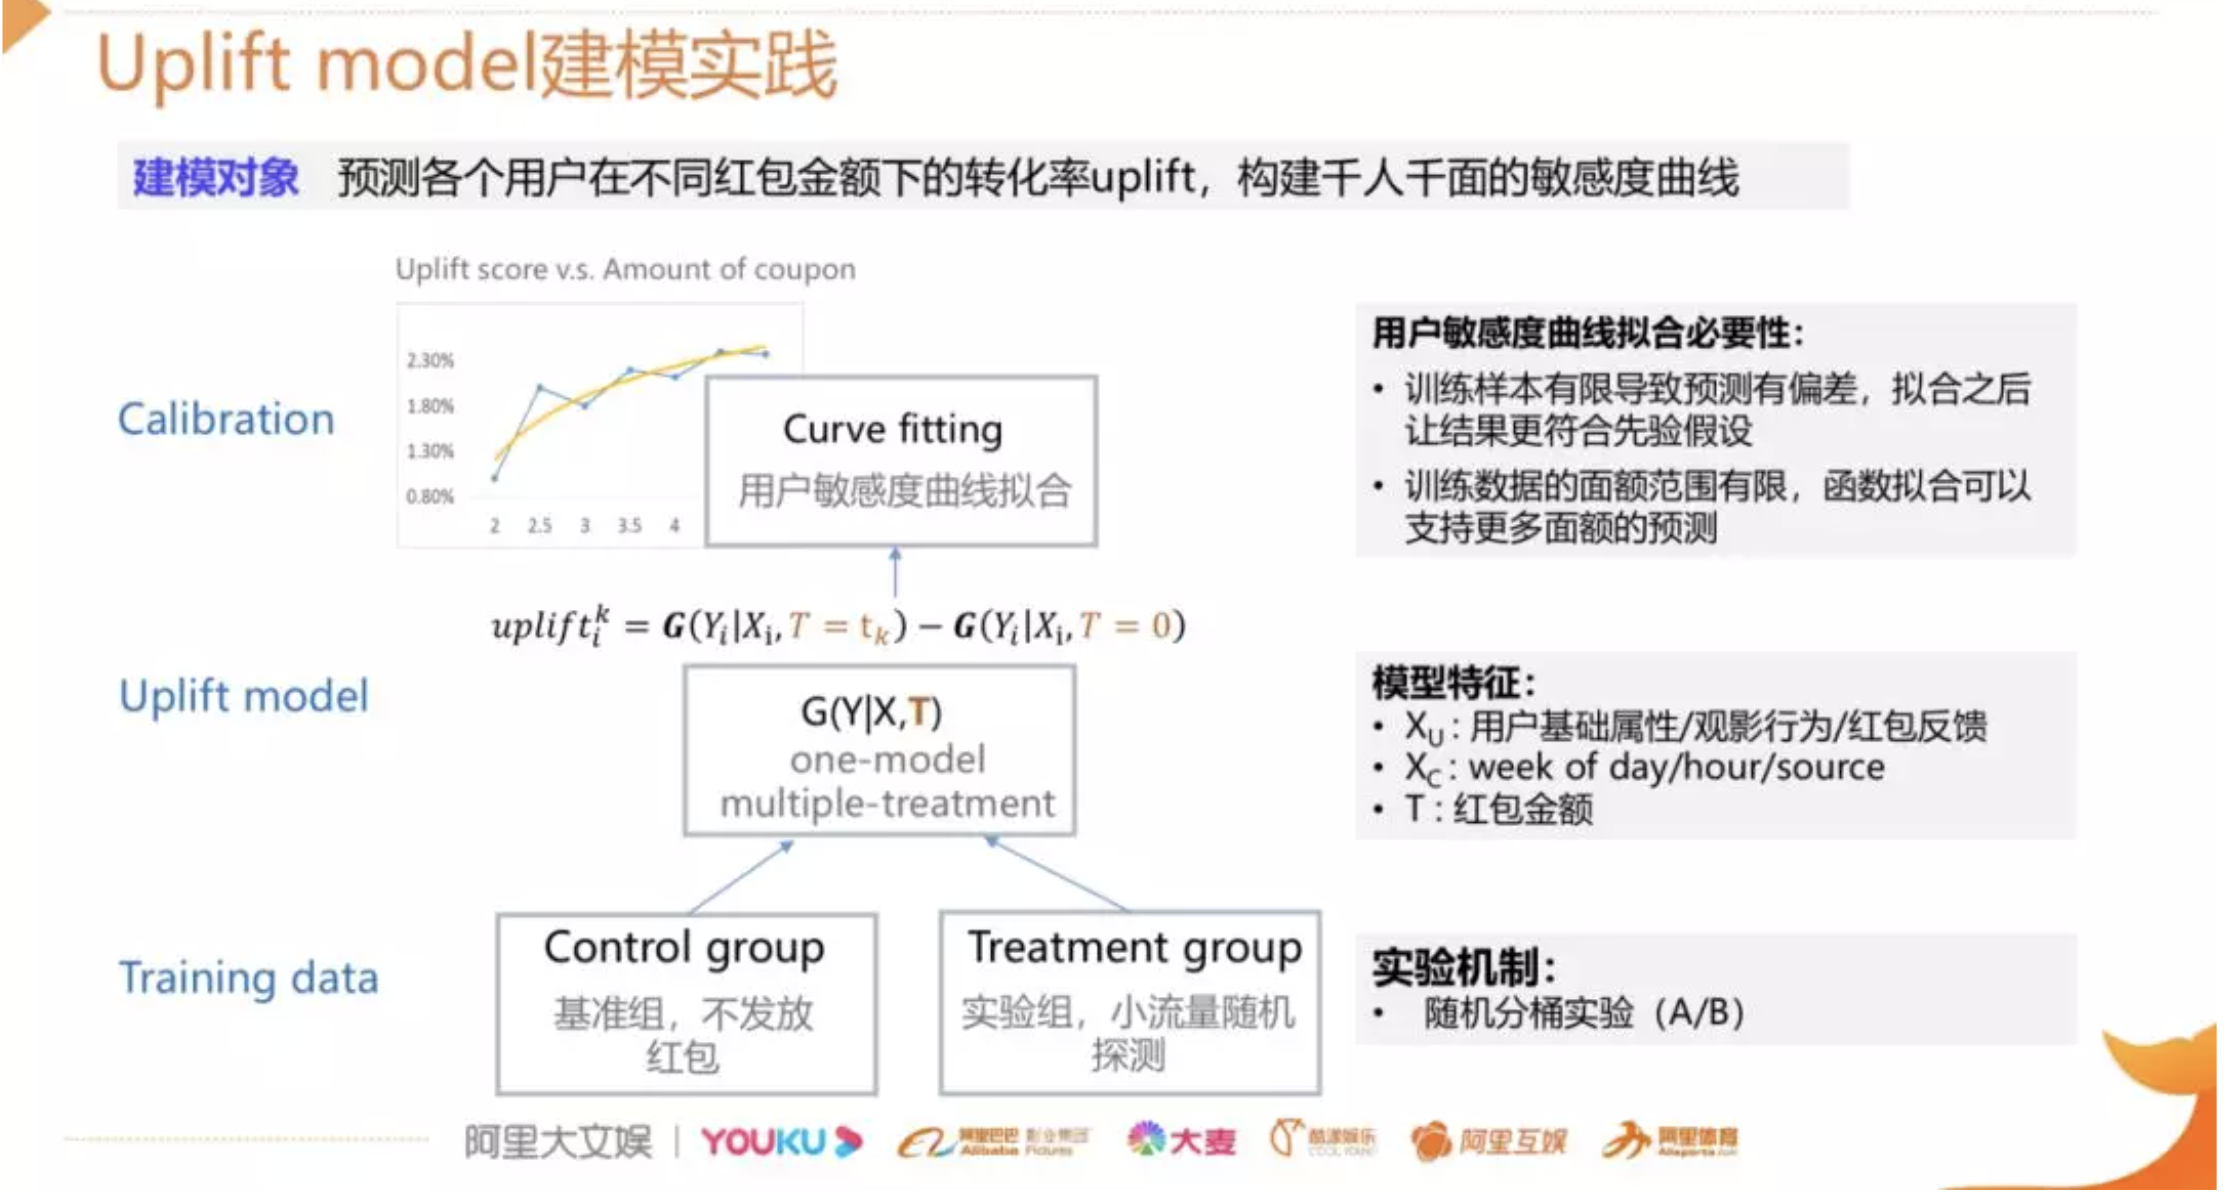
\includegraphics[width=1\textwidth]{fig/CasualInference-Uplift-Model-In-Ali3.png}
\end{figure}

我们将建模的任务拆分成三个步骤:

\textbf{ Step 1. 收集训练样本}

训练样本的收集和我们的实验是强相关的,我们采用的是随机化的分桶实验,它有两个好处,一是可以严谨公平地进行效果的评估,二是可以为uplift model的建模提供无偏的样本。建模中control组我们取的是随机化实验中的基准组,这部分用户是不进行红包发放的,而treatment组选用的是随机化实验中专为uplift model建模预留的一小部分随机探测的流量,之所以没有用有算法干预下的样本是因为用户的发放的面额与用户的特征是强相关的,并不满足CIA条件,因此这一部分样本虽然量较大,但是不能用于训练。

\textbf{ Step 2. 模型的构建和训练}

收集到样本之后可以进行建模,考虑到业务迭代的周期,我们使用的是前面介绍的One Model的差分响应模型,特征层面,除了user维度的基础属性,还有历史的观影行为,以及历史红包的反馈,同时也会引入线上实时的环境特征,最重要的是跟营销相关的特征T,目前T代表的是红包的金额。

\textbf{ Step 2. 面向业务层的模型校准和优化}

理论上到模型训练完成,就可以直接把模型放到线上去应用了,但是在离线调研时,我们发现一个问题,我们绘制的用户敏感度曲线和我们的预期不太一样,并不是严格的平滑递增的走势。我们分析有两个可能的原因:

一是与我们整体的样本规模比较有限有关,因为这种无偏样本目前大概只有几百万的量级;

二是由于用户行为的稀疏性,在这种场景下我们比较难收集到用户在不同面额下的历史数据,因此也会加剧这种不平滑性。

针对该问题,我们做了校准处理,把原始曲线做了一个函数的拟合,一方面可以让结果更加符合我们先验的假设,一方面经过这种函数化之后可以在后续支持更多面额的预测,但这种做法是否是最优的还值得进一步探讨。

\begin{figure}[H]
    \centering
    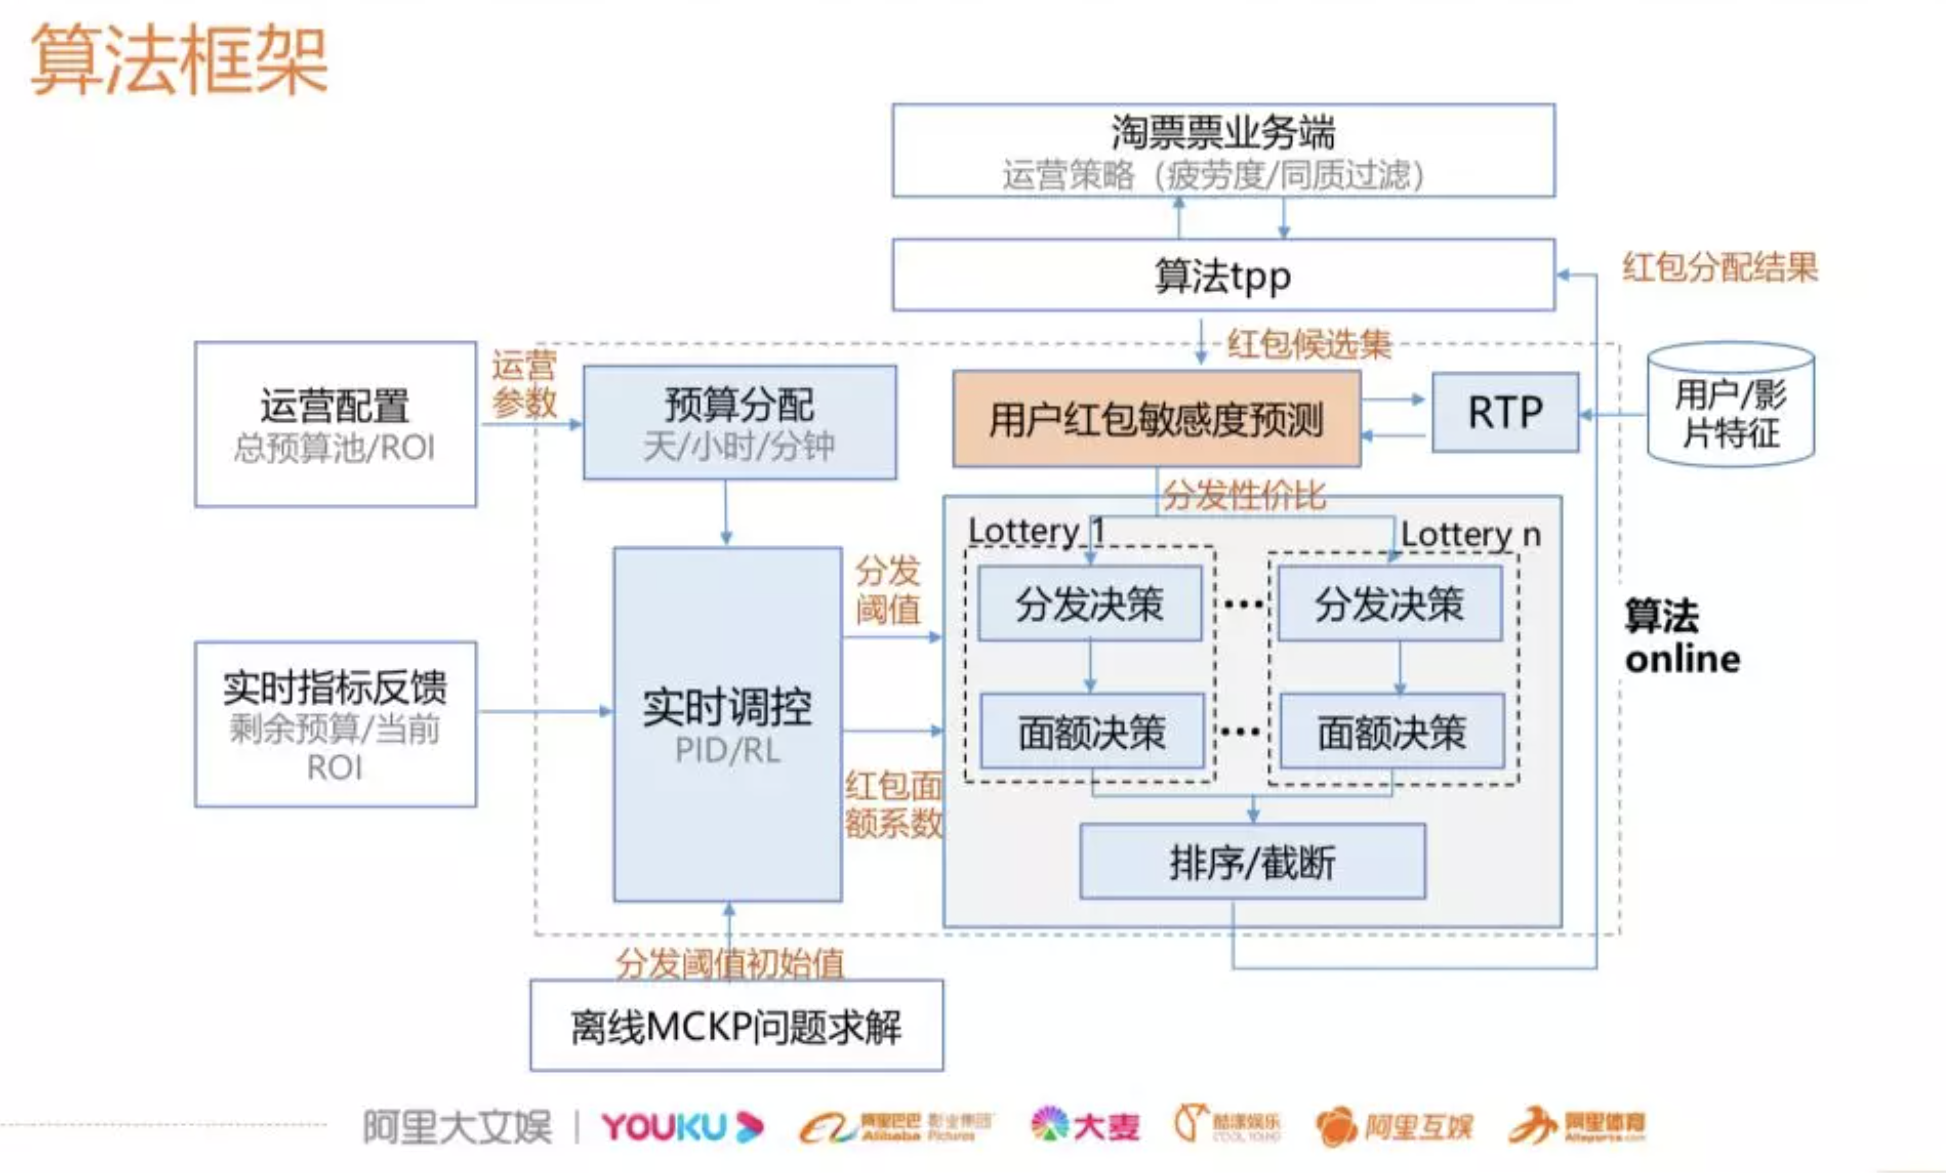
\includegraphics[width=1\textwidth]{fig/CasualInference-Uplift-Model-In-Ali4.png}
\end{figure}

模型在线上应用的框架图,如上图所示,黄色区域是基于uplift model的实时预测的模块,当一条用户的请求过来的时候,我们会实时去数据库中取用户的特征以及影片的特征,同时结合当前的环境特征预测用户在当前状态下真实的敏感度,基于这个敏感度可以进行后续分发的面额决策等。

\textbf{技术思考与后续规划}

之后智能营销的发展态势是营销手段会越来越复杂,玩法也会越来越多,比如之前我们发放的更多是平台的通用券,后面也会发一些和影片相关的影片券或者影院券,这意味treatment的维度是在不断增长的,除了红包的金额之外还需要考虑不同的红包类型,这会给算法带来两个方面的挑战,一是我们需要对问题的建模形式做一个升级,除了之前单一维度的建模之外,我们可能还要考虑多维度的建模,同时维度的剧增会对样本的量级要求越来越高,样本的稀疏性问题会更加严重,针对这个问题我们有两个可能的解法:

(1) 可以采用多任务学习的方式,联合其他场景一起建模缓解单场景样本的压力,同时也可以通过人为构造无偏样本的方式增加整体的样本量。当然除了技术侧,整个营销上面还有非常多很有意思的研究方向,比如之前更多考虑的是单个营销场景,但其实多个场景下怎么去建模和刻画他们之间的相互影响也是非常有意思的课题;

(2)我们之前uplift model建模更多考虑的是单次或者短期用户行为的增益,但实际上的营销往往是常态化或持续化的,用户的心智可能会不断发生变化,如何去建模长期的uplift也值得进一步去探讨。

\section{DiDi Food中的智能补贴实战漫谈\cite{Causal_Inference_In_DiDi}}
\subsection{差异化定价的经济学原理}
提起营销手段,第一个想到总会是差异化定价。而提起差异化定价,人们的第一印象往往是价格歧视等类似的负面印象。\textbf{其实,差异化定价的本质还是在为消费者,用户和社会创造更多的价值}。这背后是有着一套在收益管理学(Revenue Management)下最直观明了的经济学原理的。
\begin{figure}[H]
    \centering
    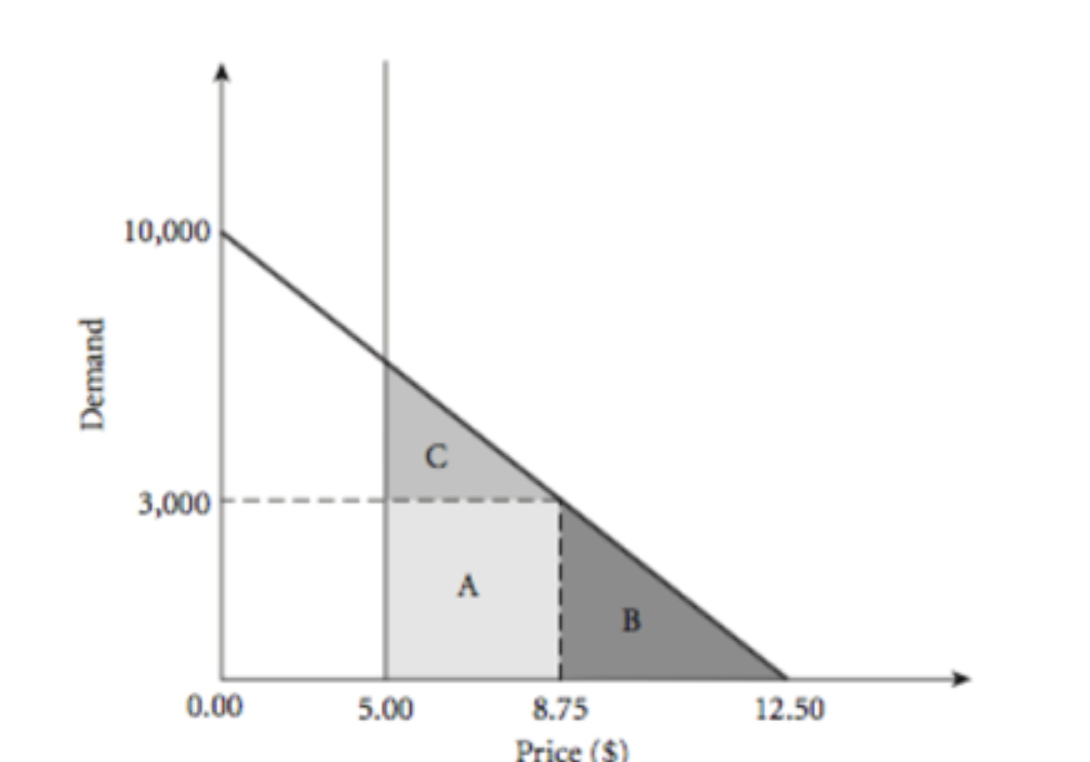
\includegraphics[width=.6\textwidth]{fig/Causal_Inference_In_DiDi_1.png}
\end{figure}
举个例子,图中所示为某商品需求(Demand)随价格(Price)变化的趋势,其中该商品的成本为\$5。简单计算可以得知在单一定价下,图中:A:所示面积即为总利润;B:所示面积为消费者剩余(Consumer Surplus);C:所示面积即为潜在收益空间

这里的消费者剩余是一个经济学上的概念,简单理解为消费者对于商品的价值评估减去商品价格,比如,一份黄焖鸡米饭,我认为它值20块钱,而它的标价是15块钱,那么20-15=5元就是消费者剩余。经济学中,一次交易只有在消费者剩余>=0的情况下才会发生。这里更深层的理解我们不去深究,简单一点我们可以将消费者剩余理解为游戏中的快乐度。一次交易中的消费者剩余越大,消费者对本次消费行为就容易觉得满意和高兴。从这个角度出发,消费者剩余本身也是商品交易行为为社会创造的价值的一部分。

那么当我们对该商品进行差异化定价,即增加了一个新的定价\$7后,
\begin{figure}[H]
    \centering
    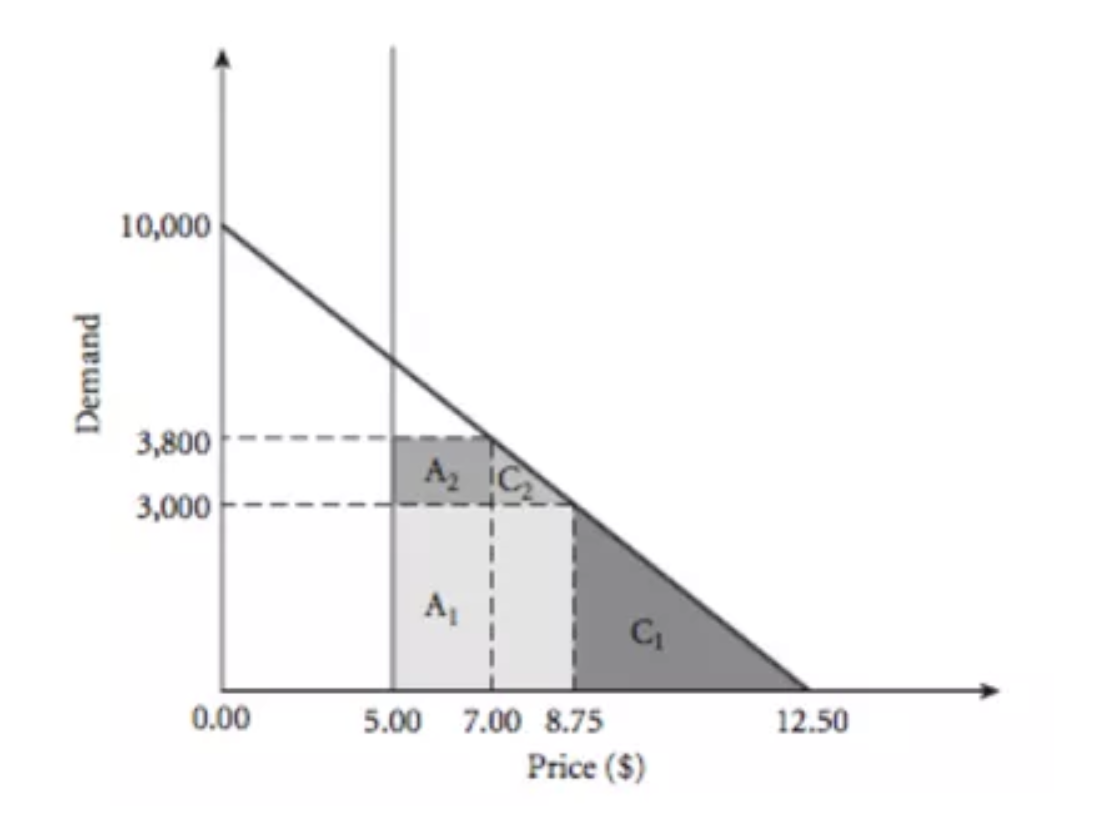
\includegraphics[width=.6\textwidth]{fig/Causal_Inference_In_DiDi_2.png}
\end{figure}
A2:所示面积即为增加的总利润;C2:所示面积即为增加的消费者剩余。

通过差异化定价,整个交易的总利润(A1+A2>A)增加了,企业和平台可以利用多出的总利润提升自己的产品与服务质量,为用户创造更多的价值。与此同时,更多的用户买到了商品,享受到了服务,整个交易的消费者剩余(C1+C2>B)也增加了。

而这,也恰恰是对差异化定价产生的社会价值最直观的解释。

\subsection{差异化定价在DiDi Food中的抓手}
DiDi Food作为国际化外卖平台,其用户面对的商品定价更多层面上是一系列服务和商品的综合定价:

P = Pi + Pd - Subsidyc

其中,Pi 为菜品标价,Pd为配送费,Subsidyc为C侧补贴。

这也为我们在商户侧(B),用户侧(C),骑手侧(D)三端进行差异化定价提供了抓手。
\begin{figure}[H]
    \centering
    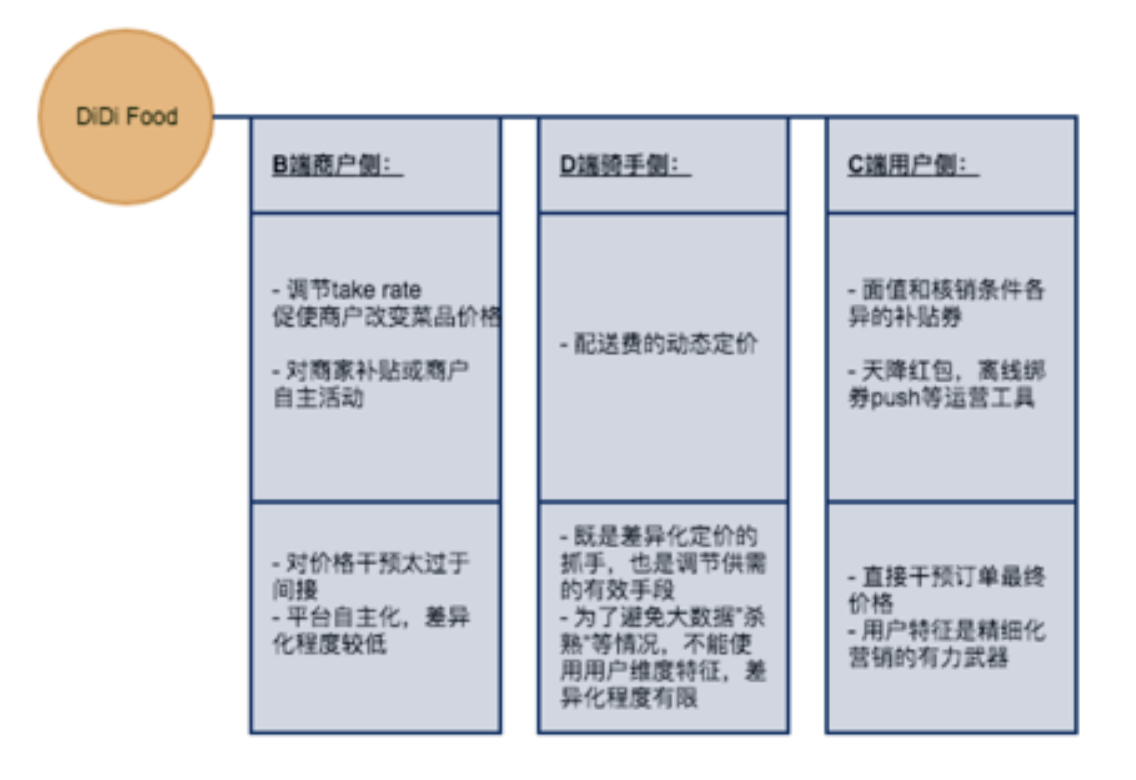
\includegraphics[width=.6\textwidth]{fig/Causal_Inference_In_DiDi_3.png}
\end{figure}

可以看到,在B侧,由于平台侧不可能拥有菜品的定价权,我们的差异化定价的选择相对比较单一并且过于间接,而且在本质上也无法达到差异化定价的目的;而在D侧,配送费的动态定价除了可以帮助平台调节供需外,其本身无疑也是一个比较有力的差异化定价的手段。但是它的使用却有着显而易见的约束,比如为了避免在配送费定价的时候产生所谓的“大数据杀熟”,我们一般不会使用用户维度的特征,而且在每一次动态调节的背后,都会有相应的价格Buffer层做调价缓冲。

因此,相对于B侧的间接影响和D侧的诸多约束,通过对用户发券进行补贴无疑是一种更为直接和更为有效的差异化定价手段。

\subsection{补贴问题的定义}
与机器学习传统三大方向【推荐,搜索,广告】不同,补贴问题中最核心和最关键的一点是补贴这个行为需要付出【成本】。这个概念的引入使得我们必须要将对这部分【成本】的使用效率作为一个核心指标,也就是所谓的「ROI」。
\begin{figure}[H]
    \centering
    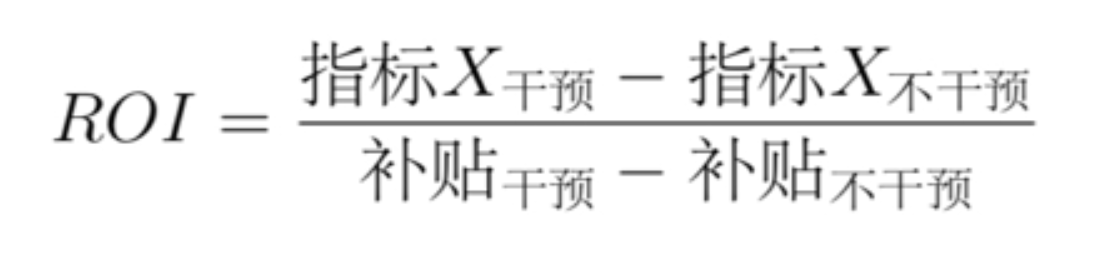
\includegraphics[width=.6\textwidth]{fig/Causal_Inference_In_DiDi_4.png}
\end{figure}
也就是衡量增加的补贴【成本】所带来【增量】指标收益。

对于这个指标的优化,一个直观的解法就是随机AB实验,通过足够多的,设计逻辑严密的,随机性完美的AB实验,我们一定可以在这个指标的优化上取得令人满意的结果。但是这个方法在具体业务中的问题是它太过于奢侈了,无论是在预算还是在时间上。

因此,为了可以高效低廉地求解这个问题,我们可以将优化目标拆解为两个子问题:
\begin{itemize}
\setlength{\itemsep}{0pt}
\setlength{\parsep}{0pt}
\setlength{\parskip}{0pt}
    \item \textbf{预估干预的Action相比于没有干预时带来的【增量】;}
    \item \textbf{在存在多种干预【Action】和已预估了它们【增量】的情况下,如何为每个用户合理分配【Action】以期望达到全局最优;}
\end{itemize}

\textbf{对于问题a}:与传统机器学习解决的问题不同,子问题a所面临的一个终极难题是,我们想要预估的这个【增量】在观察数据中是没有真值的。如果是一条被干预后的样本,我们只能观察到它被干预后的指标而无从得知它不被干预时的指标。同样,如果是一条未被干预的样本,在观察数据中我们也无法得知它被干预后的表现是怎样的。这也正是在因果推断理论中因果关系阶梯的第三层所提到【反事实 (Counterfactuals)】。而对这个“增量“预估的问题,业界也提出不少了的解法,我们会在之后尝试做出更详细的介绍。

\textbf{对于问题b}:熟悉运筹相关知识的同学很容易就可以看出这是一个比较经典的,在约束下求解全局最优的问题。从整数规划到Exploit\&Explore到强化学习,在这个问题下可以探索的方向也有很多。这里也会在后面给出我们的一些实践。

\subsection{DiDi Food中智能补贴的架构与流程}
在DiDi Food中,与智能补贴相关的工程架构如图:
\begin{figure}[H]
    \centering
    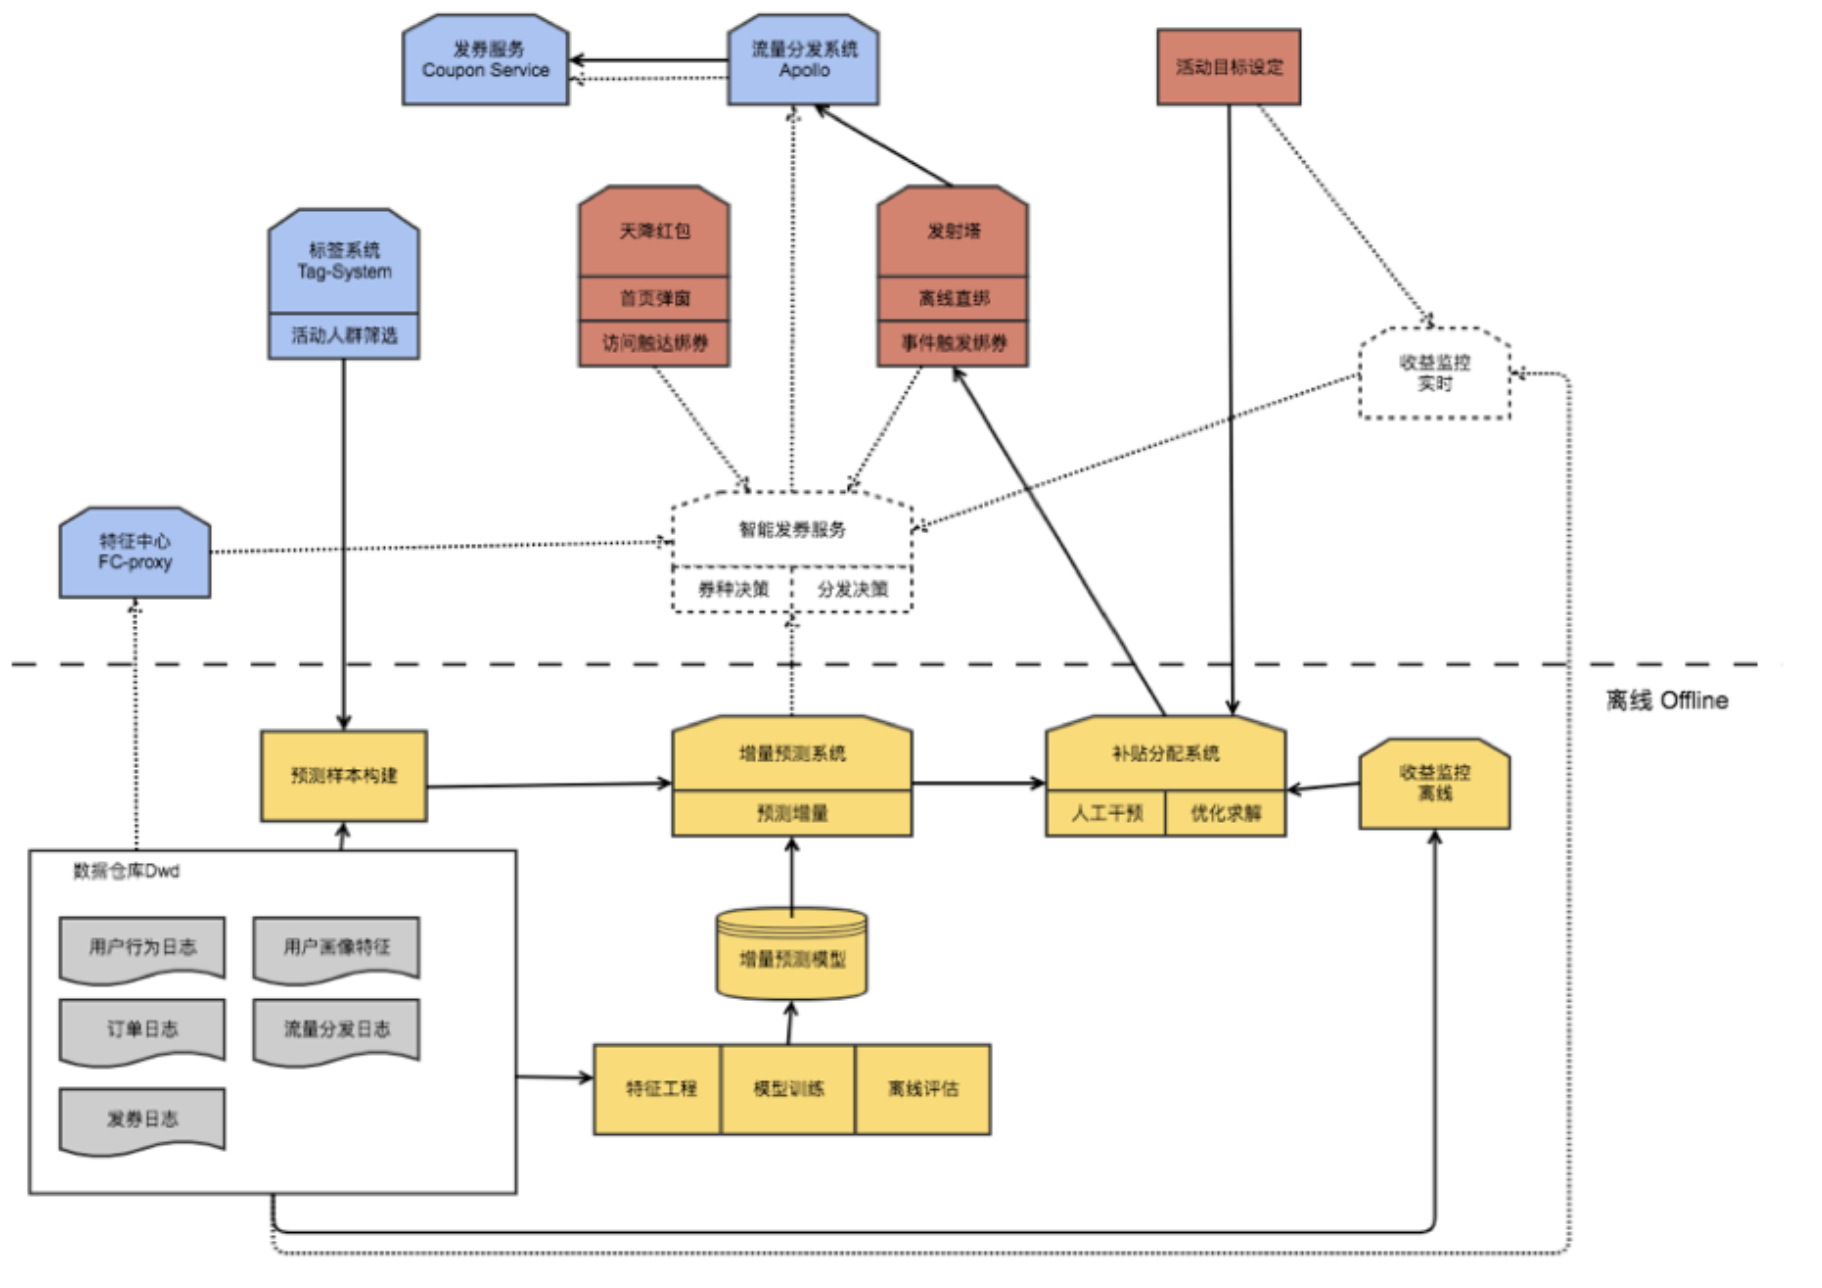
\includegraphics[width=1\textwidth]{fig/Causal_Inference_In_DiDi_5.png}
\end{figure}

其中,虚线部分为正在规划和开发中的线上智能决策模块。而【增量预测】和【补贴分配】则是这个框架中最核心的部分,分别用于解决上面所拆分出的子问题a和b。

对于【增量预测】模块中使用的模型,更细节的训练和更新流程如下:
\begin{figure}[H]
    \centering
    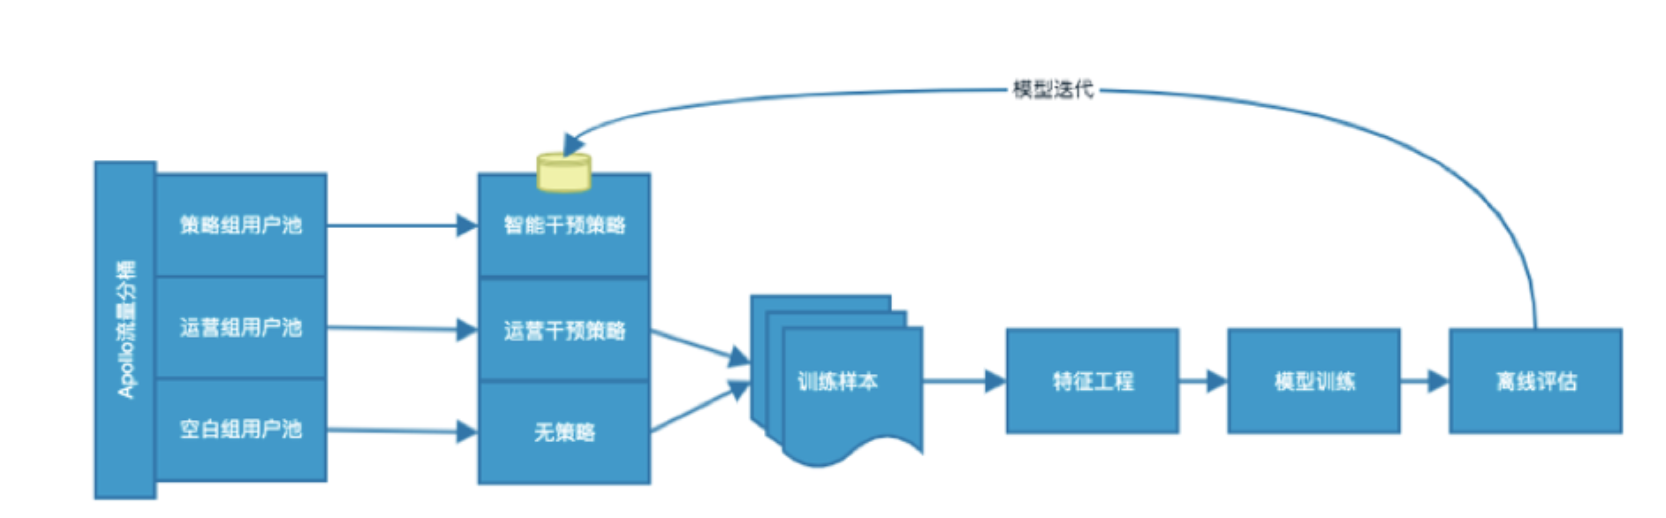
\includegraphics[width=1\textwidth]{fig/Causal_Inference_In_DiDi_6.png}
\end{figure}

其中,在特征筛选方面:由于我们所使用的部分候选模型并非是直接对【增量】进行建模,而是使用多种模型间接地近似这个【增量】。因此,我们无法如一般线性或者树模型一样直接产出所有特征对于最终输出【增量】的重要度。我们在实践中使用的方法是用一个新的LightGBM去拟合离线评估最优模型产出的【预测增量】,并用这个新模型的特征重要度来近似评估各个维度特征的重要性,以此来决策是否加入和剔除特征。选择LightGBM的原因是我们对于这个模型的精度并没有太高的要求,相反我们希望它能够比较快速地在训练流程中对新加入特征的给出反馈。LightGBM高效地训练速度和不需要过多特征工程的优点比较契合我们的需求。

另外,在样本构建方面,从流程图中可以看到,在构建训练样本和离线评估测试样本时,我们剔除了那些被线上模型干预后的样本。这是因为在理论上,我们是在三个假设的前提下去使用模型拟合一个在观察数据中并不存在的【增量】的。
\begin{figure}[H]
    \centering
    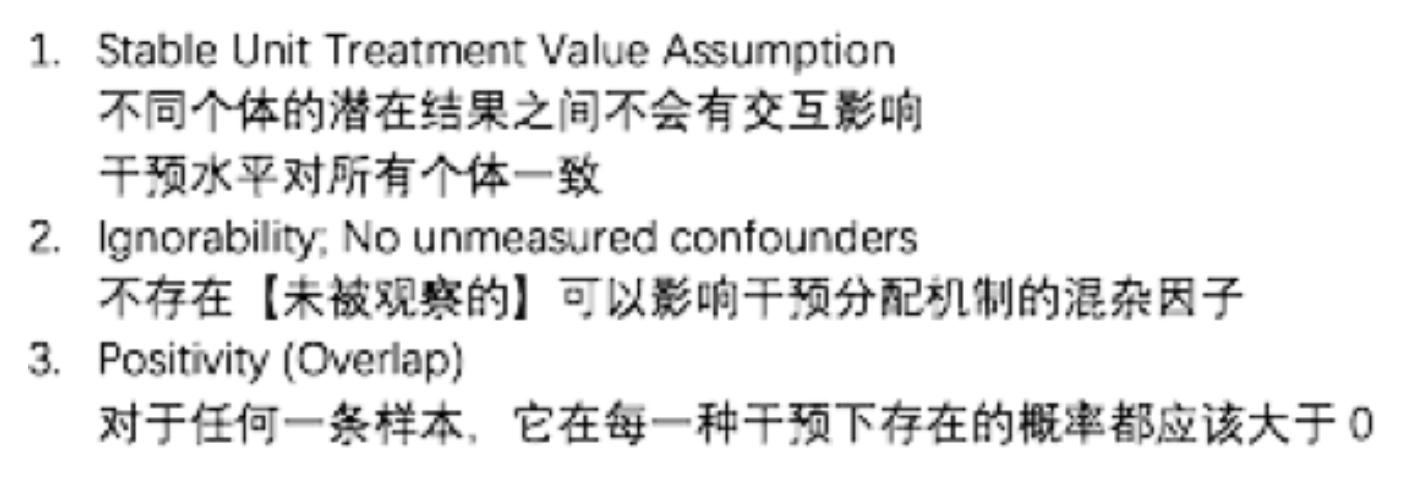
\includegraphics[width=1\textwidth]{fig/Causal_Inference_In_DiDi_7.png}
\end{figure}

其中,针对其中第二条假设,我们的个人理解是我们虽然允许有影响分配机制的特征存在,但是我们需要将这些特征也纳入我们的观察。在模型干预的数据样本中,影响干预分配机制的往往是模型产出的【预测增量】。这个特征我们没有也无法将其纳入我们的观察。因此,我们将这部分样本从训练和测试样本中剔除了。

这点在数据结果上也可以看出,对于同一个批次的样本,同一套参数同一套模型,评估样本中【干预后样本】的存在会导致离线评估的结果大相径庭,从而影响我们离线评估和判断模型优劣。

另外在同一个测试样本上,有该类【干预后样本】样本参与训练的模型的离线效果也出现了比较明显的下降。

*离线评估指标为AUUC,其介绍将会在后面给出

同样模型,评估样本中有无干预样本:
\begin{figure}[H]
    \centering
    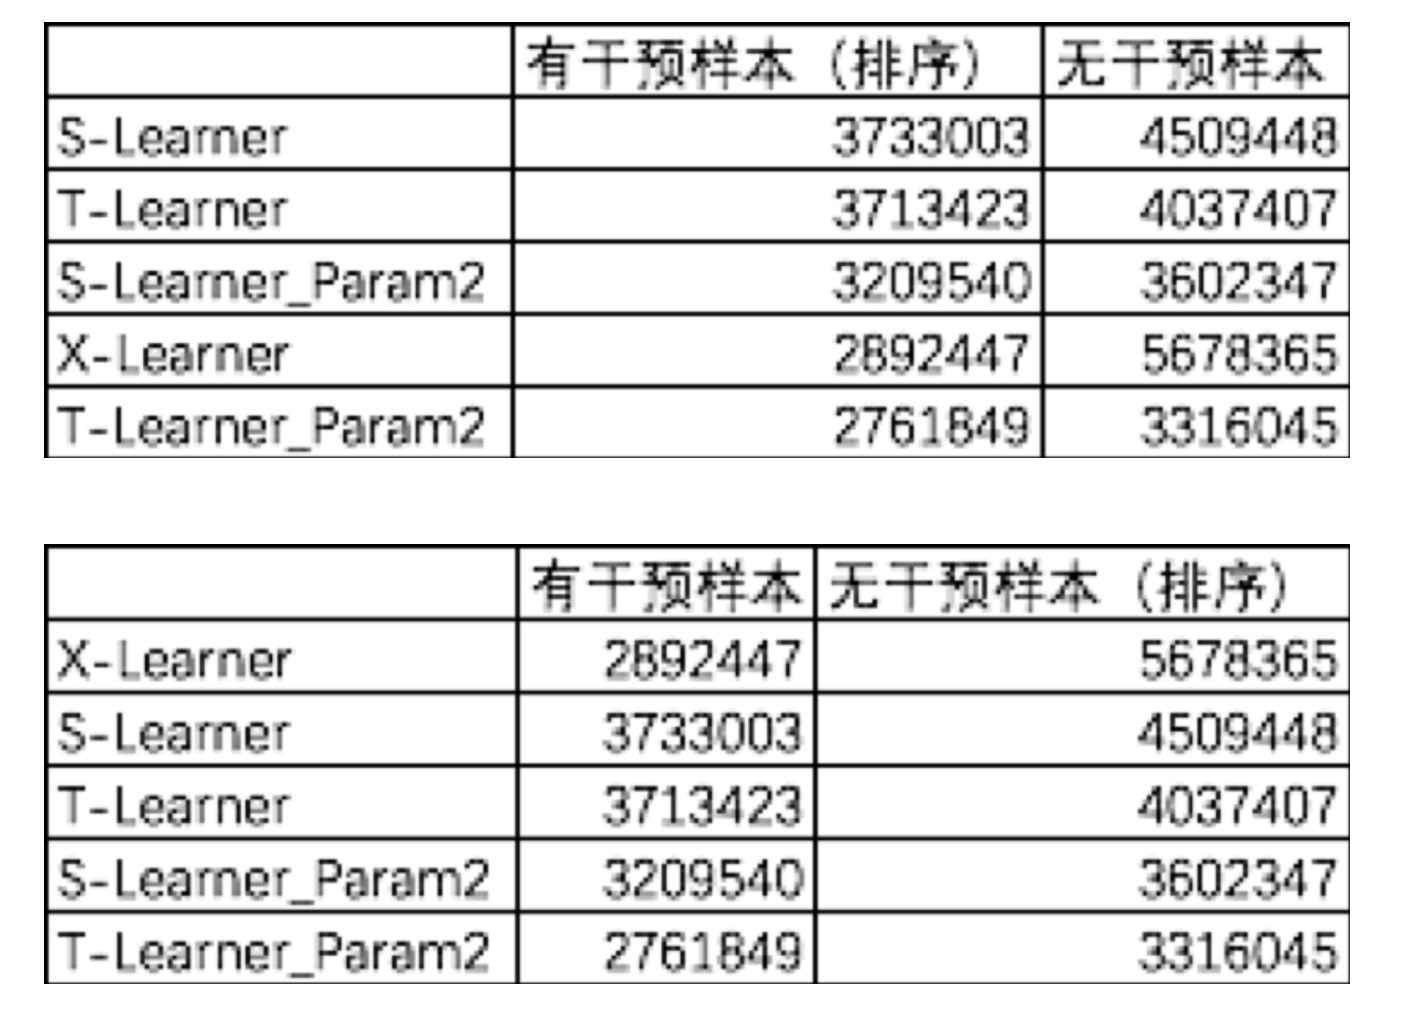
\includegraphics[width=.6\textwidth]{fig/Causal_Inference_In_DiDi_8.png}
\end{figure}

同样测试集,干预样本是否参与训练:
\begin{figure}[H]
    \centering
    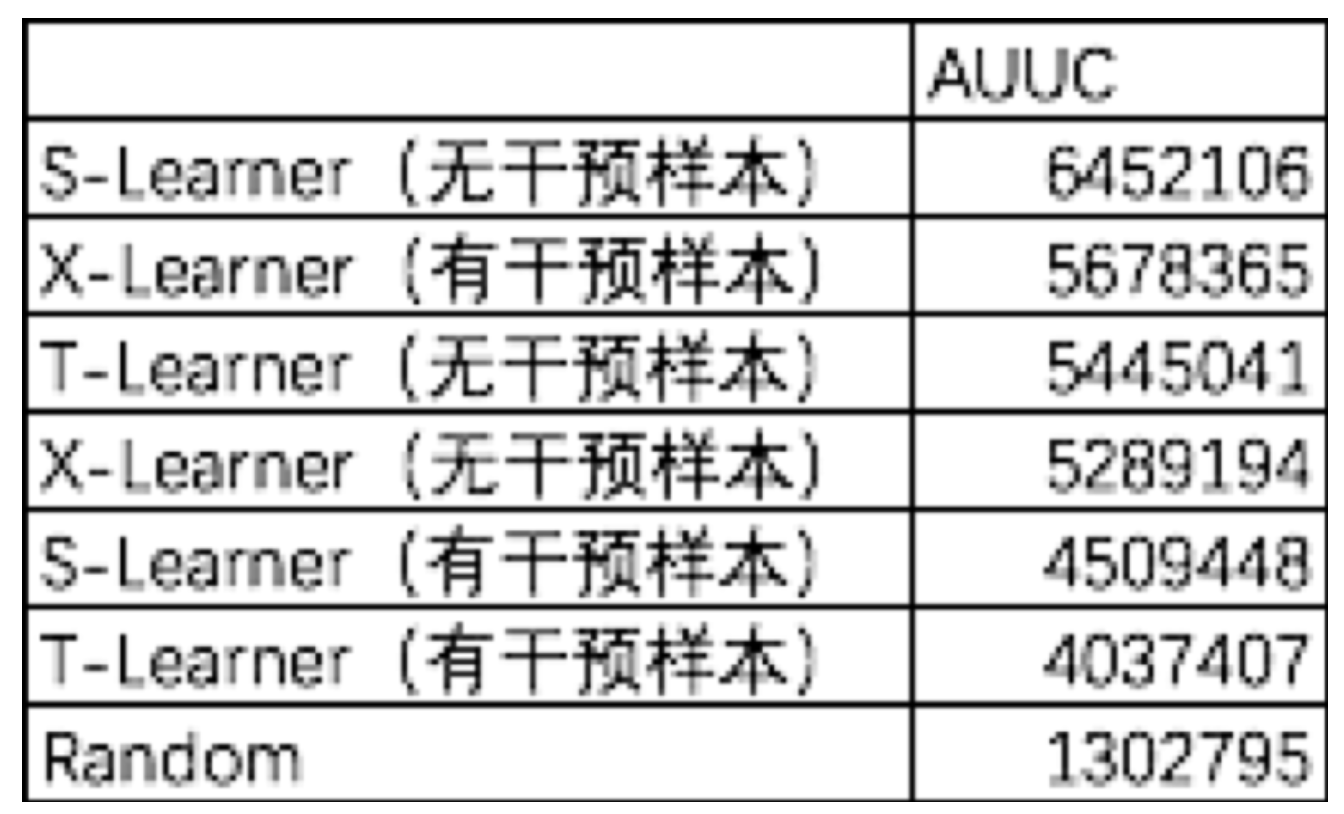
\includegraphics[width=.6\textwidth]{fig/Causal_Inference_In_DiDi_9.png}
\end{figure}
我们将在下一部分详细介绍增量预估中所使用的算法。

\subsection{增量预估}
在营销补贴活动中,我们常常使用模型预测用户在有补贴下的交易意愿,并对交易意愿强的用户发放补贴,以促进用户完成交易行为。这中间,我们往往会忽略一个重要的问题,即用户在无补贴下的交易意愿。在有成本的补贴活动中,我们希望把补贴发给补贴敏感的用户,即我们希望发放的补贴能够真正撬动了原本不会产生交易行为的用户,从而达到差异化定价的目的。那么,在此基础上,我们可以根据用户是否有补贴和是否下单,将其划分为四种人群:
\begin{figure}[H]
    \centering
    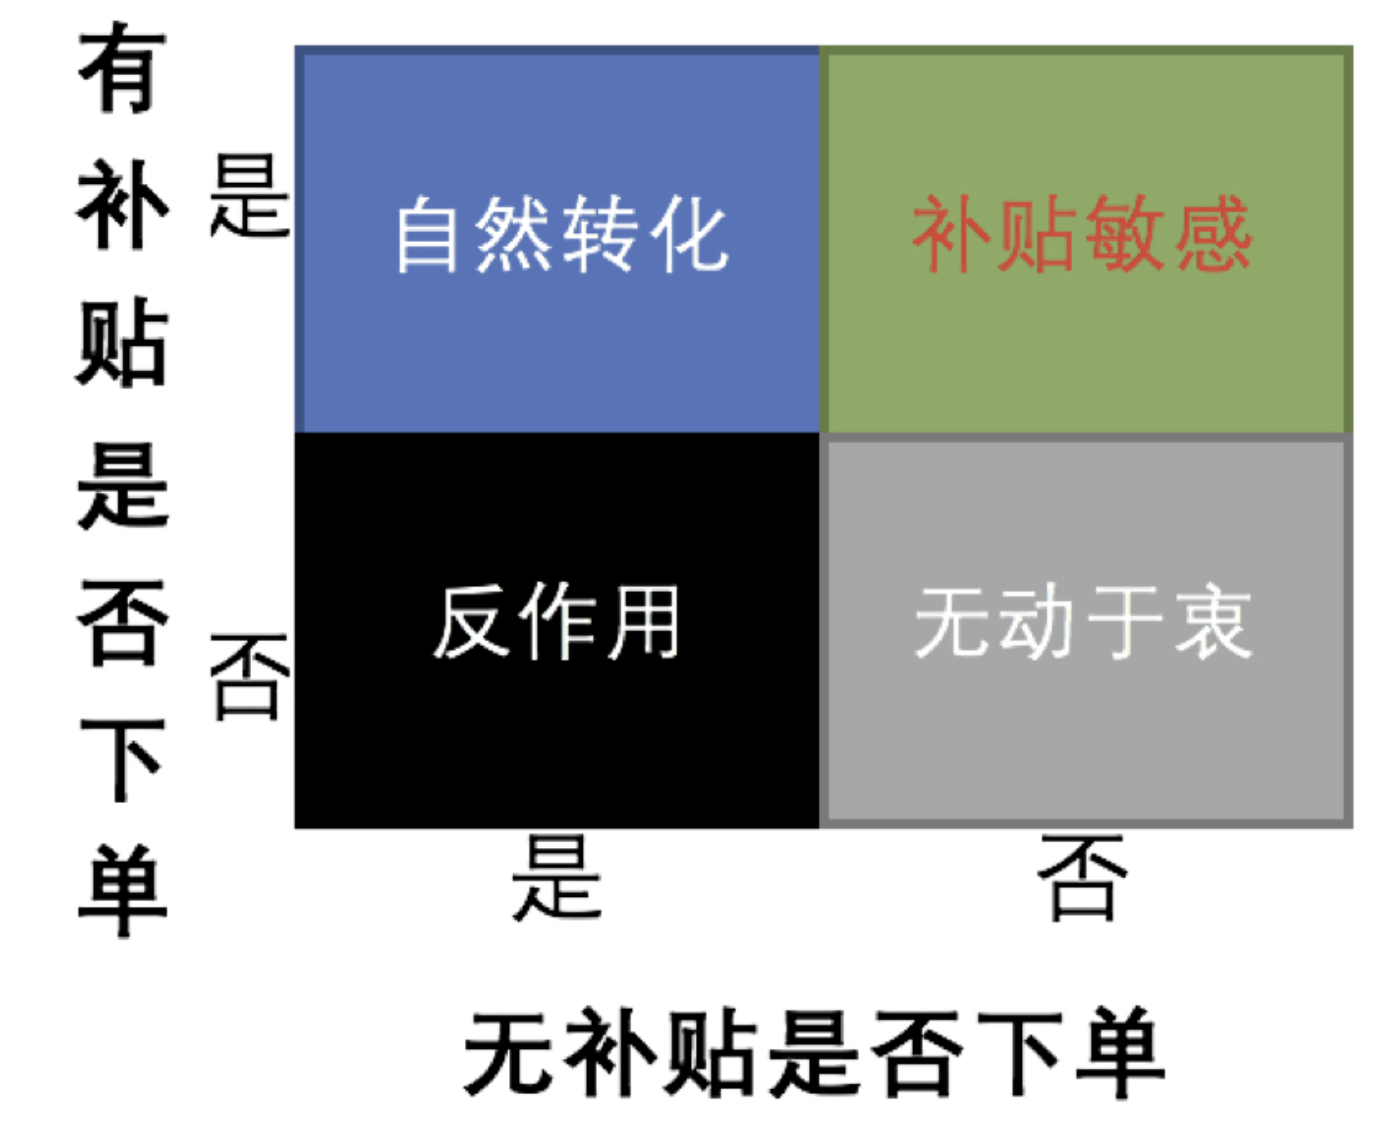
\includegraphics[width=.6\textwidth]{fig/Causal_Inference_In_DiDi_10.png}
\end{figure}

如之前所述,在补贴活动中,我们希望只触达【补贴敏感人群】。传统模型只预测交易意愿,无法预测因为补贴活动提升的交易意愿,也就无法很好的区分开来四种人群。为了能够获取因为补贴活动提升的交易意愿,我们引入了 Uplift Model。

Uplift Model 是对某种干预带来的【增量(Uplift)】进行建模的方法;它主要用于去预测补贴活动提升的交易意愿,也即前文描述的【增量(Uplift)】,并通过预测的结果去识别哪些用户能够真正为补贴活动所撬动。

设 $W=1$ 表示有补贴,$W=0$ 表示无补贴,$X$ 表示用户,$Y=1$ 表示购买。则 Uplift Model 可表示为:

补贴活动提升的购买意愿 = $P(Y = 1|X,W = 1) − P(Y = 1|X,W = 0)$

根据其实现方法可分为两大类:Meta-Leaner 和 Tree-Base。

Meta-Learner 是基于传统分类和回归算法组合建模,间接去预测增量;常见的 Meta-Learn 算法有 Two Model(T-Learner),Single Model(S-Learner) ,X-Learner和R-Learner 等。

Tree-Base 则是通过树模型中节点分裂的算法思想,尝试去直接对增量建模,预测增量。

在下面的介绍中,$X_0, Y_0$ 将分别表示对照组样本特征和 Label;$X_1, Y_1$ 表示实验组样本特征和 Label。$W \in \{0, 1\}$ 则表示用户是否属于实验组。

\subsection{Meta-Learner}
如同前面介绍的那样,Meta-Learn体系内的模型主要思想都是想通过一系列的基模型(base-learner)的组合,去近似拟合一个无法被观测到的【增量(Uplift)】。我们这里将会介绍主流的四个模型,Two-Model,Single-Model,X-Learner和R-Learner。

\subsubsection{Two Model}
Two Model 算法也称为差分模型,顾名思义就是利用两个模型的差值去近似用户的增量。这也是最符合直觉的一种思路。具体模型构造流程是:

(1) 对实验组数据和对照组数据分别建立模型
$$
\hat{\mu}_0 = f(X_0, Y_0)
$$
$$
\hat{\mu}_1 = f(X_1, Y_1)
$$

(2) 用实验组模型$\hat{mu}_1$预测值减去对照组模型$\hat{mu}_0$预测值去近似增量$\hat{\tau}$
$$
\hat{\tau}(x) = \hat{\mu}_1(x) - \hat{\mu}_0(x)
$$

\textbf{优点}:

– 简单直观,易实现。

– 可直接使用现有分类算法。

\textbf{缺点}:

– 双模型存在误差累加。

– 间接计算增量,无法对模型进行优化。

\subsubsection{Single Model}
Single Model\textbf{将与干预手段W有关的特征加入训练,只建立一个模型}。这样做的好处是,相较于Two Model,我们可以减少模型较多带来的误差累加。

具体模型构造流程是:

(1) 在实验组和对照组样本特征中加入 $W$ 有关的特征,将实验组和对照组的样本特征、Label 合并,训练一个模型$\hat{mu}$;

(2) 通过对用户的特征 $W$ 赋值$W=1$和$W=0$计算用户增量:
$$
\hat{mu}(x) = \hat{mu}(x, W = 1) - \hat{mu}(x, W = 0)
$$

与 Two Model 相比,Single-Model也可以直接使用现有分类算法,同时也减少了 Two Model 带来的误差累积问题;另外,由于它利用了全量数据训练模型,因此也进一步提高了模型的泛化能力。但是,它依然是对增量间接建模,无法根据增量优化模型,并且也同样存在着模型精度问题。

\textbf{优点}:

– 简单直观,易实现。

– 可直接使用现有分类算法。

– 减少双模型误差累加。

– 训练样本增加,提高模型精度。

\textbf{缺点}:

– 间接计算增量,无法根据增量对模型进行优化.

\subsubsection{X-Learner}
X-Learner算法是在Two Model模型基础上提出的,基于\textbf{利用观察到的样本结果去预估未观察到的样本结果的思想,对增量进行近似,同时还会对结果进行倾向性权重调整,以达到优化近似结果的目的}。

具体模型构造流程是:

(1) 对实验组和对照组分别建立两个模型$\hat{mu}_1$和$\hat{mu}_0$:
$$
\hat{\mu}_0 = f(X_0, Y_0)
$$
$$
\hat{\mu}_1 = f(X_1, Y_1)
$$

(2) 利用实验组模型$\hat{mu}_1$预测对照组样本在实验组的转化率$\hat{mu}_1(X_0)$减去对照组Label $Y_0$ 得到对照组近似增量 $D_0$;

利用对照组模型$\hat{mu}_0$预测实验组样本在对照组的转化率$\hat{mu}_0(X_1)$,由实验组 Label $Y_1$ 减去$\hat{mu}_0(X_1)$得到实验组近似增量$D_1$。
$$
D_0 = \hat{\mu}_1(X_0) - Y_0
$$
$$
D_1 = Y_1 -  \hat{\mu}_0(X_1)
$$

(3) 对求得的实验组和对照组增量$D_1$和$D_0$建立两个模型$\hat{\tau}_1$和$\hat{\tau}_0$。
$$
\hat{\tau}_0 = f(X_0, D_0)
$$
$$
\hat{\tau}_1 = f(X_1, D_1)
$$

\begin{framed}
对于与  two model 的区别为:two model 中,$f$ 是对$X_0, Y_0$ 进行建模,X-Learner 中,$f$ 是对 $X_0, D_0$(也就是增量)进行建模。
\end{framed}

(4) 引入倾向性得分模型 $e(x)$ 对结果进行加权,求得增量。
$$
e(x) = P(W=1|X=x)
$$
$$
\hat{\tau}(x) = e(x) \hat{\tau}_0(x) + (1- e(x)) \hat{\tau}_1(x)
$$

算法的优点之一是在步骤(3)中,我们得到了两个近似的增量值,并直接对其建模。\textbf{如果我们本身对业务有足够的了解,知道增量的一些相关先验知识(线性/非线性等),那么这些先验知识是可以参与建模过程并帮助我们提升模型精度的}。与此同时,在理论上,它也解决了对照组和实验组样本差别较大场景下预测增量精度问题,但它并没有说明多大差别才适用X-Learner,我们在实际应用中的离线评估部分,X-Learner虽然偶尔表现优异,但并没有持续显著优于其他模型。

\textbf{优点}:

–适合实验组和对照组样本数量差别较大场景。

– 对于增量的先验知识可以参与建模,并且引入权重系数,减少误差。

\textbf{缺点}:

– 多模型造成误差累加。

\subsubsection{R-Learner}
R Learner 算法思想不同于Two、Single和X-Learner。其核心思想是通过 Robinson’s transfomation 定义一个损失函数,然后通过最小化损失函数的方法达到对增量进行建模的目的。

(1) 训练倾向性得分模型 $e(x)$
$$
e(x) = P(W=1|X=x)
$$ 

(2) 通过CV方式对Label Y的期望$m^*$建模
$$
m^* = \mathbb{E}[Y|X=x]
$$

(3) 通过求得的$e(x)$和$m^*(x)$,优化如下损失函数
$$
\tau^*(\cdot) = \arg\min_{\tau}\Bigg\{\frac{1}{n}\sum_1^n\Big((Y_i - m^*(X_i)) - (W_i - e^*(X_i))\tau(X_i)\Big)^2 + \Lambda(\tau(\cdot))\Big\}
$$

这一部分在实现时,我们可以看成是用带权重的$X$去拟合
$$
\tau(X_i) = \frac{Y_i  - m^*(X_i)}{W_i - e^*(X_i)}
$$

训练中$X_i$的权重为
$$
(W_i - e^*(X_i))^2
$$

\textbf{优点}:

– 灵活且易于使用。

– 损失函数可以接深度网络等。

\textbf{缺点}:

– 模型精度依赖于$m^*(x), e^*(x)$的精度。

\subsection{Tree-Based Model}
传统机器学习模型中,\textbf{树模型主要的思路就是通过对特征点进行分裂,将$X$划分到一个又一个subspace中,这与补贴场景下,希望找到某一小部分增量很高的用户的想法几乎是完美重合}。因此,与meta-learner不同的是,uplift model下的树模型希望通过这样的分裂方式达到对增量直接建模的目的。
\begin{figure}[H]
    \centering
    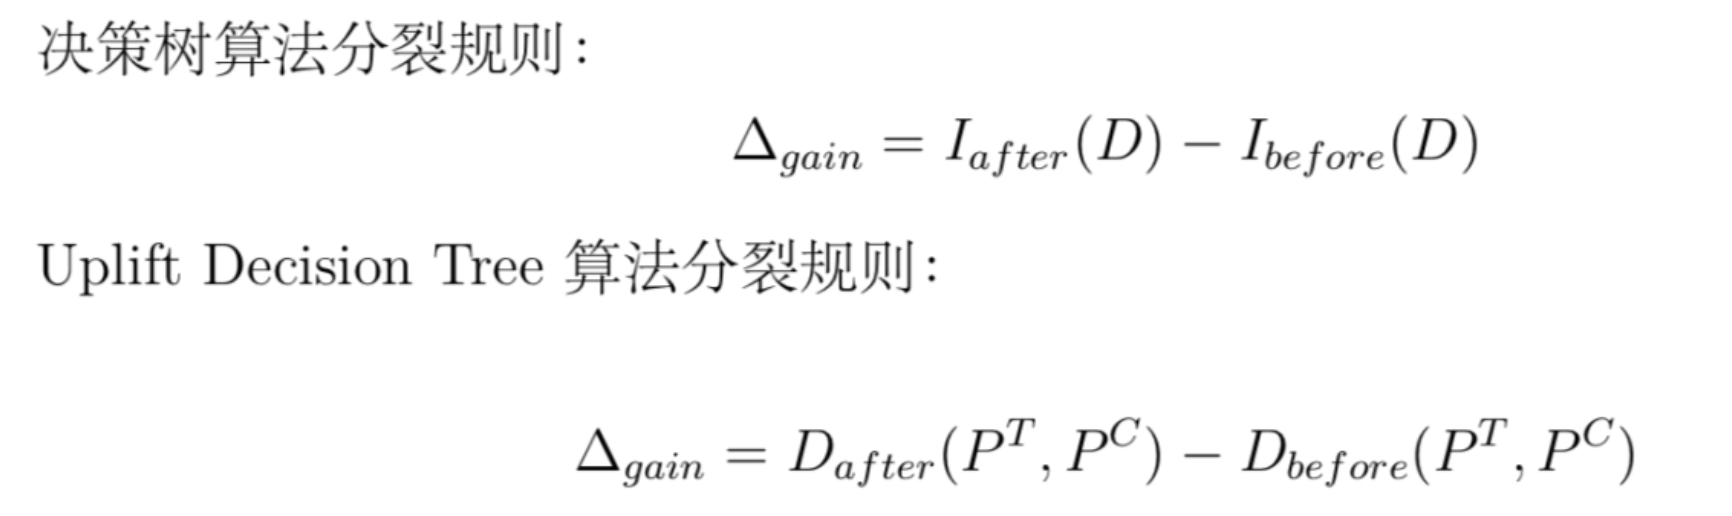
\includegraphics[width=.6\textwidth]{fig/Causal_Inference_In_DiDi_11.png}
\end{figure}

传统分类树模型是希望通过信息理论(information theory)中的信息熵等思想,用计算信息增益的方法去解决分类问题。而在uplift tree model中,其本质也还是想要通过衡量分裂前后的变量差值去决策是否分裂节点,不过\textbf{这里的这个决策差值的计算方法不再是信息增益(information gain),而是不同的直接对增量uplift建模的计算方法,其中包括了利用分布散度对uplift建模和直接对uplift建模}。

\subsubsection{分布散度下的uplift tree}
分布散度是用来度量两个概率分布之间差异性的值,当两个分布相同时,两个离散分布的散度为非负且等于零。我们可以把实验组和对照组理解为两个概率分布,然后利用分布散度作为非叶节点分裂标准,最大化实验组和对照组的样本类别分布之间的差异,减少样本不确定度。常见的分布散度有KL 散度 (Kullback-Leibler divergence)、欧式距离 (Squared Euclidean distance) 和卡方散度(Chi-squared divergence),在uplift model中,其具体计算方法如下:
\begin{figure}[H]
    \centering
    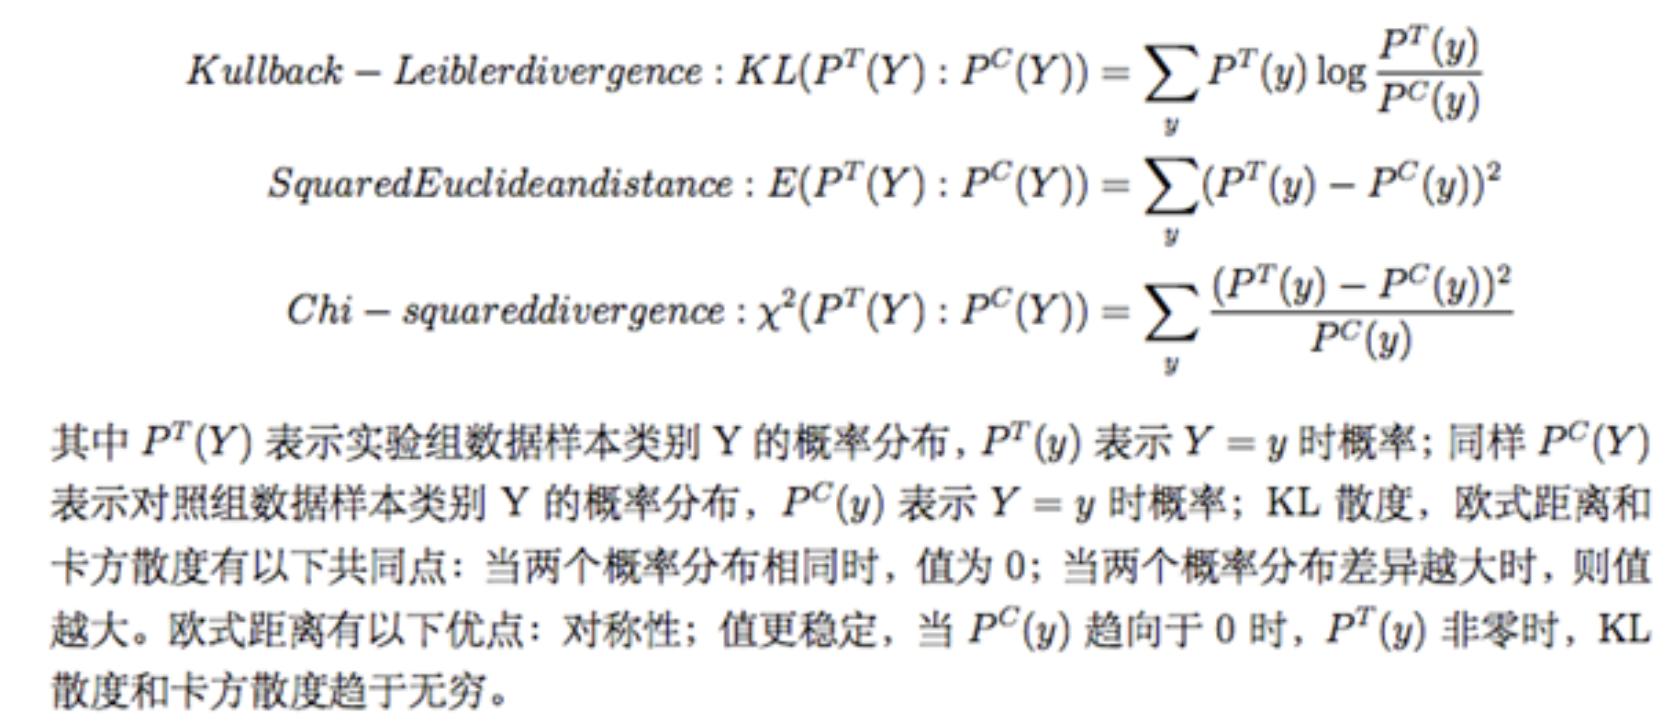
\includegraphics[width=1\textwidth]{fig/Causal_Inference_In_DiDi_12.png}
\end{figure}

除此以外,分布散度还有个特点:通过公式可以推导,当结点中对照组数据为空时,KL散度会退化为决策树分裂准则中的信息增益;欧式距离和卡方散度将会退化为基尼指数。而当结点中实验组数据为空时,欧式距离将会化为基尼指数。这也是该类分裂准则的优点之一。

其模型主要构造流程为:
\begin{figure}[H]
    \centering
    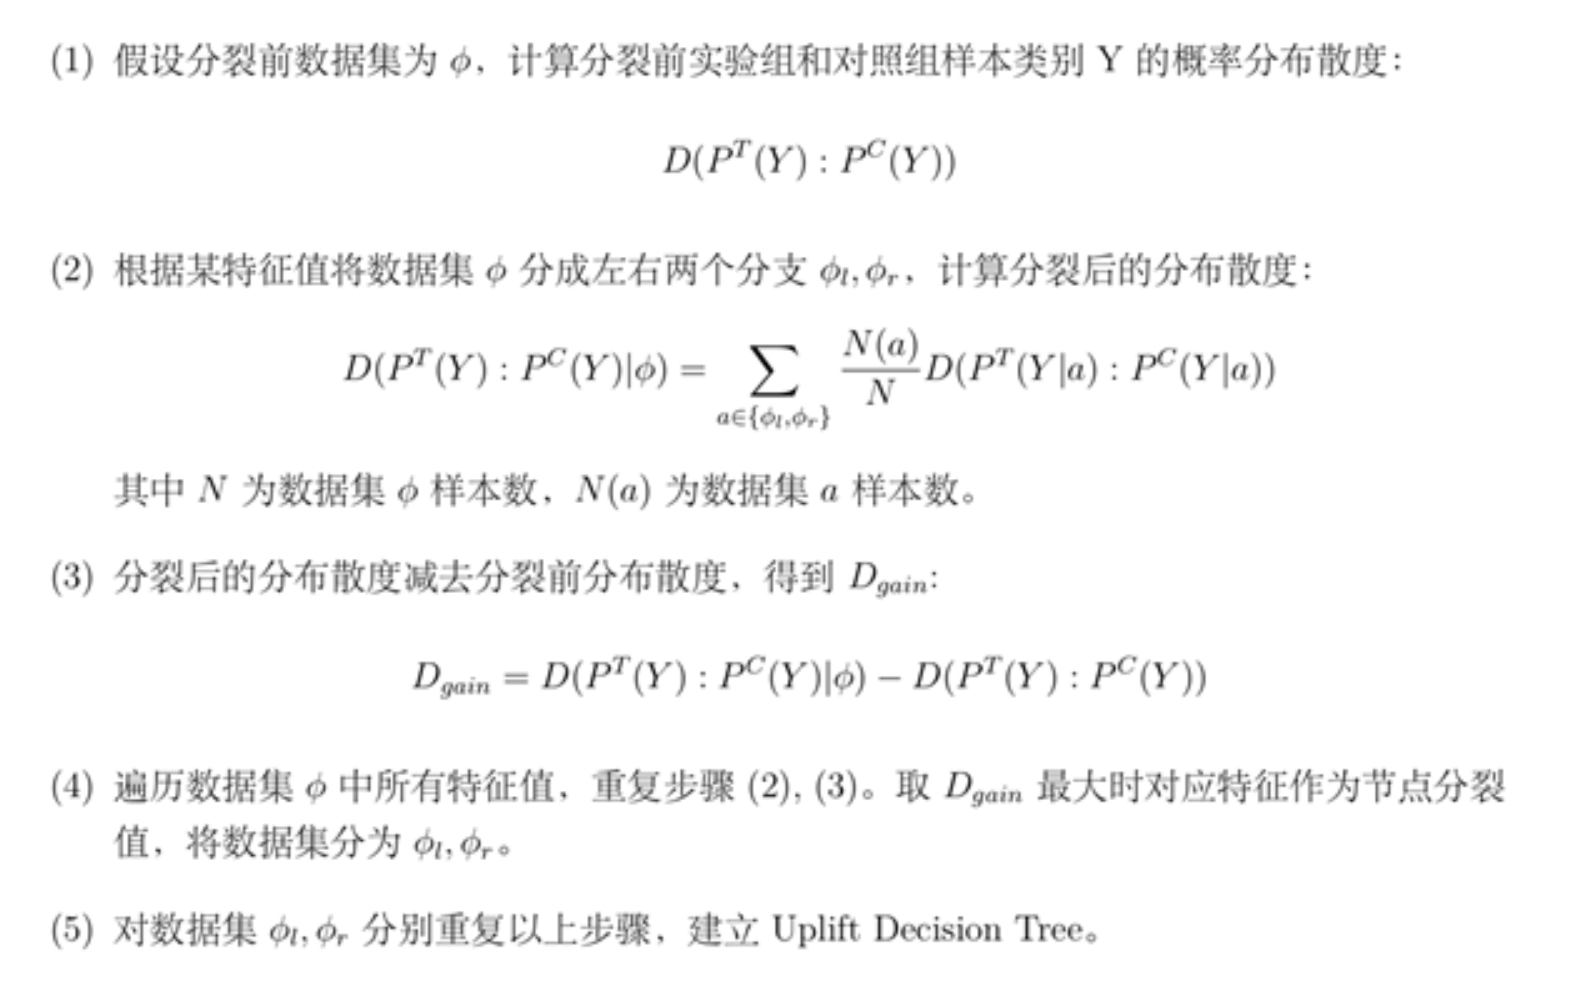
\includegraphics[width=1\textwidth]{fig/Causal_Inference_In_DiDi_13.png}
\end{figure}

算法的部分可能比较晦涩,我们可以举个例子简单描述这里所谓的分布散度的计算方法:
\begin{figure}[H]
    \centering
    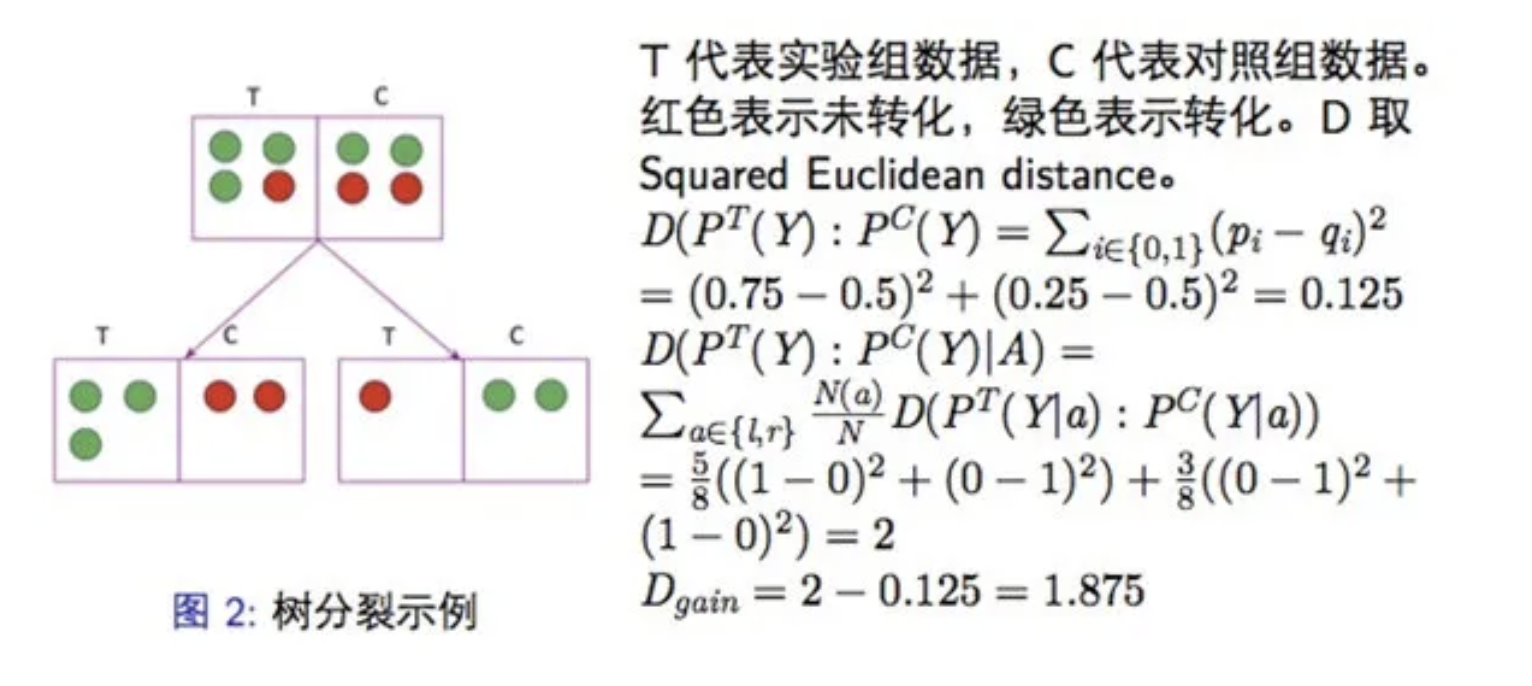
\includegraphics[width=.6\textwidth]{fig/Causal_Inference_In_DiDi_14.png}
\end{figure}

\subsection{对uplift直接建模的CTS Tree}
MIT的Zhao Yan 等人在2017年提出了一种新的名为CTS的分裂准则去构建Uplift Tree。CTS algorithm是Contextual Treatment Selection的缩写。不同于分布散度,在该标准下,我们会直接\textbf{最大化每个节点上实验组和对照组之间label期望的差值(可以理解为该节点上样本的Uplift值)},并以此来分裂节点。

CTS树具体构造流程为:
\begin{figure}[H]
    \centering
    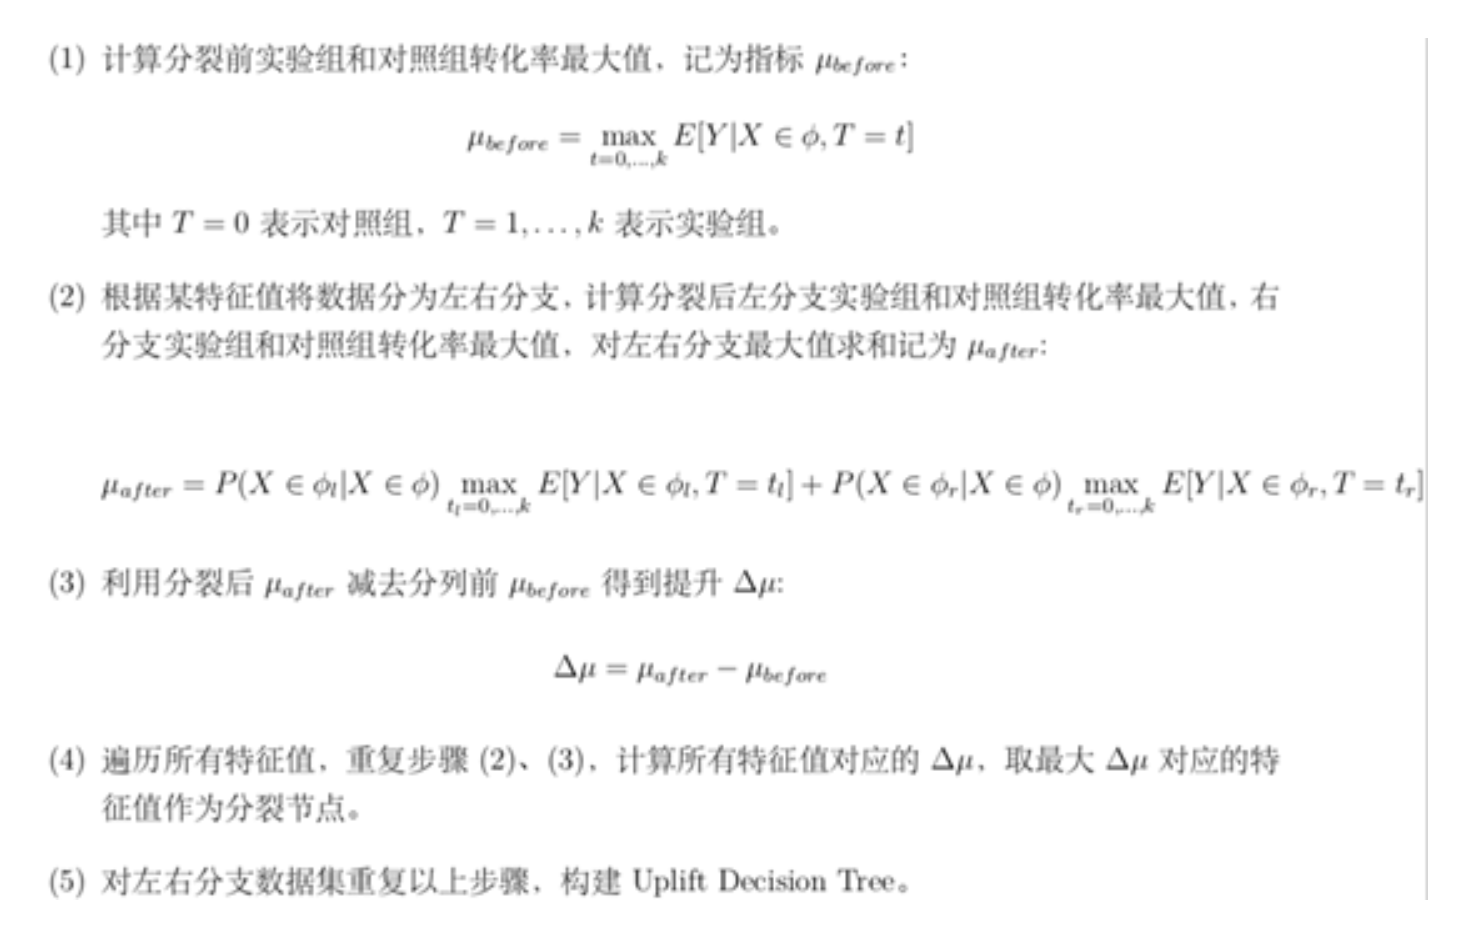
\includegraphics[width=1\textwidth]{fig/Causal_Inference_In_DiDi_15.png}
\end{figure}

相比于meta-learner,uplift下树模型由于往往是直接对uplift进行建模和利用特征直接对人群进行切分,因此模型精度往往比较高一些。但是在实际应用中,还是需要要注意树模型的收敛性以及它的泛化能力。

\subsection{Uplift Model 模型评估}
常用分类和回归算法,可以通过 AUC、准确率和 RMSE 等去评估模型的好坏。而由于Uplift Model 中不可能同时观察到同一用户在不同干预策略下的响应,即无法获取用户真实增量, 我们也就无法直接利用上述评价指标去衡量模型的好坏。因此,Uplift Model 通常都是通过划分十分位数来对齐实验组和对照组数据,去进行间接评估。常用的评估方 法有 Qini 曲线、AUUC 等。

\subsection{Qini curve}
Qini 曲线是衡量 Uplift Model 精度方法之一,通过计算曲线下的面积,类似 AUC 来评价模型的好坏。其计算流程如下

(1) 在测试集上,将实验组和对照组分别按照模型预测出的增量由高到底排序,根据用户数量占实验组和对照组用户数量的比例,将实验组和对照组分别划分为十份,分别是 Top10\%, 20\%, . . . , 100\%。

(2) 计算Top10\%,20\%,...,100\%的Qini系数,生成Qini曲线数据(Top10\%,Q(Top10\%)),
(...,...), (Top100\%, Q(Top100\%))。Qini 系数定义如下:
$$
Q(i) = \frac{n_{t,y=1}(i)}{N_t} - \frac{n_{c,y=1}(i)}{N_c}, \qquad i = 10\%, 20\%, \cdots, 100\%
$$

可以看出,\textbf{Qini 系数分母是实验组和对照组的总样本量,如果实验组和对照组用户数量差别比较大,结果将变得不可靠}。

\subsubsection{AUUC}
AUUC(Area Under the Uplift Curve) 的计算流程与 Qini 曲线的计算流程一样,计算前 10\%、20\%、. . . 、100\% 的指标,绘制曲线,然后求曲线下的面积,衡量模型的好坏。不同是 AUUC 指标计算方法与 Qini 指标计算不同,AUUC 指标定义如下:
$$
G(i) = \Big( \frac{n_{t,y=1}(i)}{N_t} - \frac{n_{c,y=1}(i)}{N_c} \Big)\Big(n_t(i) + n_c(i)\Big), \qquad i = 10\%, 20\%, \cdots, 100\%
$$

与 Qini 指标含义相同,当 i 取10\% 时,$n_t(i)$表示实验组前 10\% 用户数量,$n_c(i)$表示对照组前 10\% 用户数量。可以看出,\textbf{AUUC 指标计算方法可以避免实验组和对照组用户数量差别较大导致的指标不可靠问题}。

\textbf{值得注意的是,当分桶时,对照组边界点预估出的增量与实验组边界点的预估值有较大差别时候,以上的两个评估指标似乎都显得不那么可靠了。因此在实际中,我们使用的往往是AUUC 另外的一种计算方法}。
\begin{figure}[H]
    \centering
    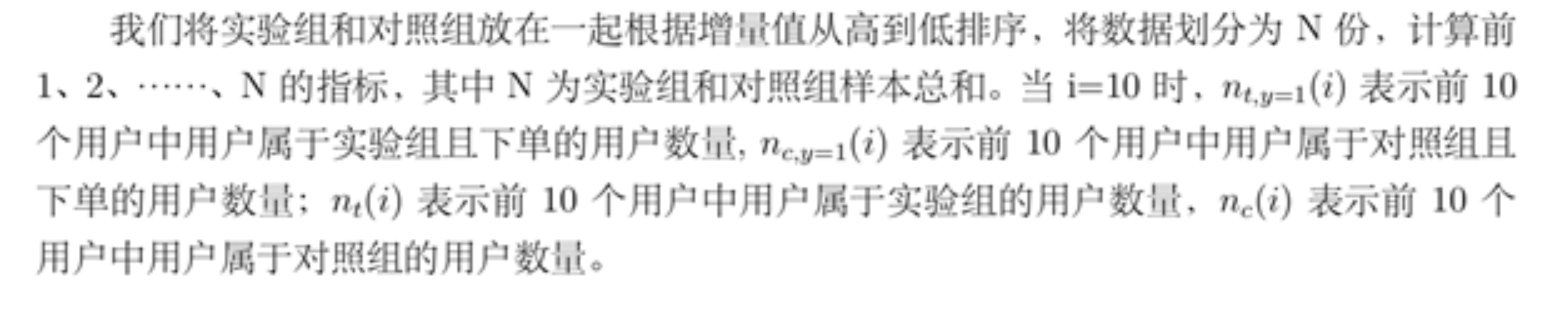
\includegraphics[width=1\textwidth]{fig/Casual_Inference_In_Didi_16.png}
\end{figure}

\subsection{分发策略}
对增量预估完毕后,接下来就需要具体地为用户池中用户分配补贴券。在基于增量预估的基础上,我们尝试了两种分发策略:

\subsubsection{贪心分配}
很多时候,运营对于使用的券类别和每个券类别的预算分配都有\textbf{比较大的限制和约束}。在这样的约束下,我们的做法是按照券值面额从低到高,为每个券类别计算可支配数量,然后对用户池所有用户按照预估出的Uplift值和计算出的可发放数量倒排截断,并将分配完毕的用户从备选用户池中移除。这样一个用户如果在\textbf{各种券类别下uplift都很高时,我们将会优先为他/她配置券值较低的补贴券}。这样做法的好处是简洁明了实现简单,在人工干预较强的时候对于运营的可解释性也比较强。缺点当然就是在自由度更高情况下,显然不能达到全局最优。

\subsubsection{整数规划}
而当我们对于预算和券种的设置拥有了更多的自主权时,我们也尝试了在预算约束下的最大化求解,具体的求解公式如下:
\begin{figure}[H]
    \centering
    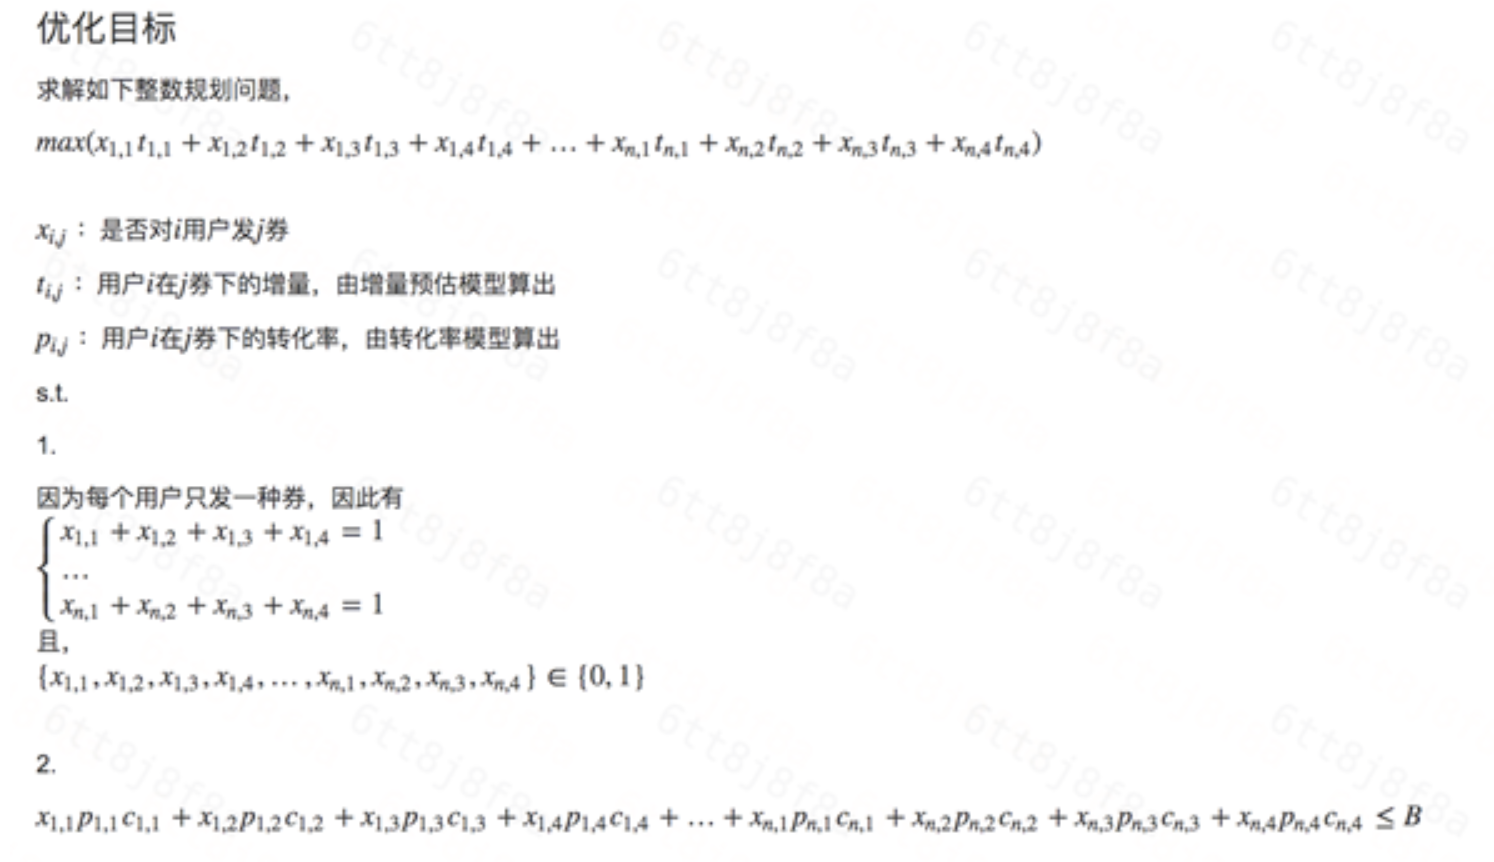
\includegraphics[width=1\textwidth]{fig/Casual_Inference_In_Didi_17.png}
\end{figure}
可以看到,这是一个\textbf{典型的整数规划求解问题}。由于目前我们单次求解用户量级基本上还是在百万量级上,因此这个模块在线下的求解时间依然可控,相信随着业务更多的拓展,我们面临的最大挑战是还是在可控时间对这个公式的求解。

\subsection{实验效果}
模型上线之后,我们在DiDi Food业务内两个不同的城市进行了不同目标约束下的AB实验,实验所有组别基于的用户群筛选条件一致,并经过Didi流量分发平台随机进入不同组别。空白组为实验期间不会受到干预的用户池,运营组为在实验期间由运营人工策略干预的用户池,策略组为实验期间策略模型分配干预的用户池。其中,空白组的存在主要是为了另外两组补贴策略计算ROI提供Base数据。

实验的主要目标分为两个方向,分别为与运营组人工策略相比,模型干预策略需要达到:
\begin{itemize}
\setlength{\itemsep}{0pt}
\setlength{\parsep}{0pt}
\setlength{\parskip}{0pt}
    \item 相同单量,更少补贴
    \item 相同补贴,更多单量
\end{itemize}

主要评价指标为:
\begin{itemize}
\setlength{\itemsep}{0pt}
\setlength{\parsep}{0pt}
\setlength{\parskip}{0pt}
    \item ROI
    \begin{figure}[H]
    \centering
    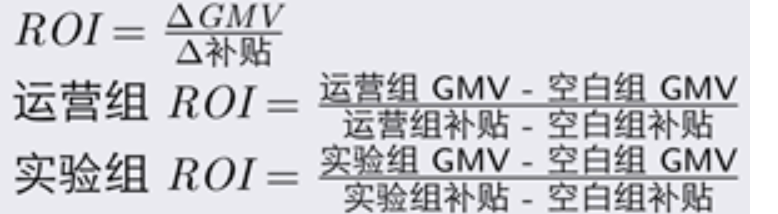
\includegraphics[width=.4\textwidth]{fig/Casual_Inference_In_Didi_18.png}
\end{figure}
    \item 补贴金额
    \item 单量
\end{itemize}

\begin{figure}[H]
    \centering
    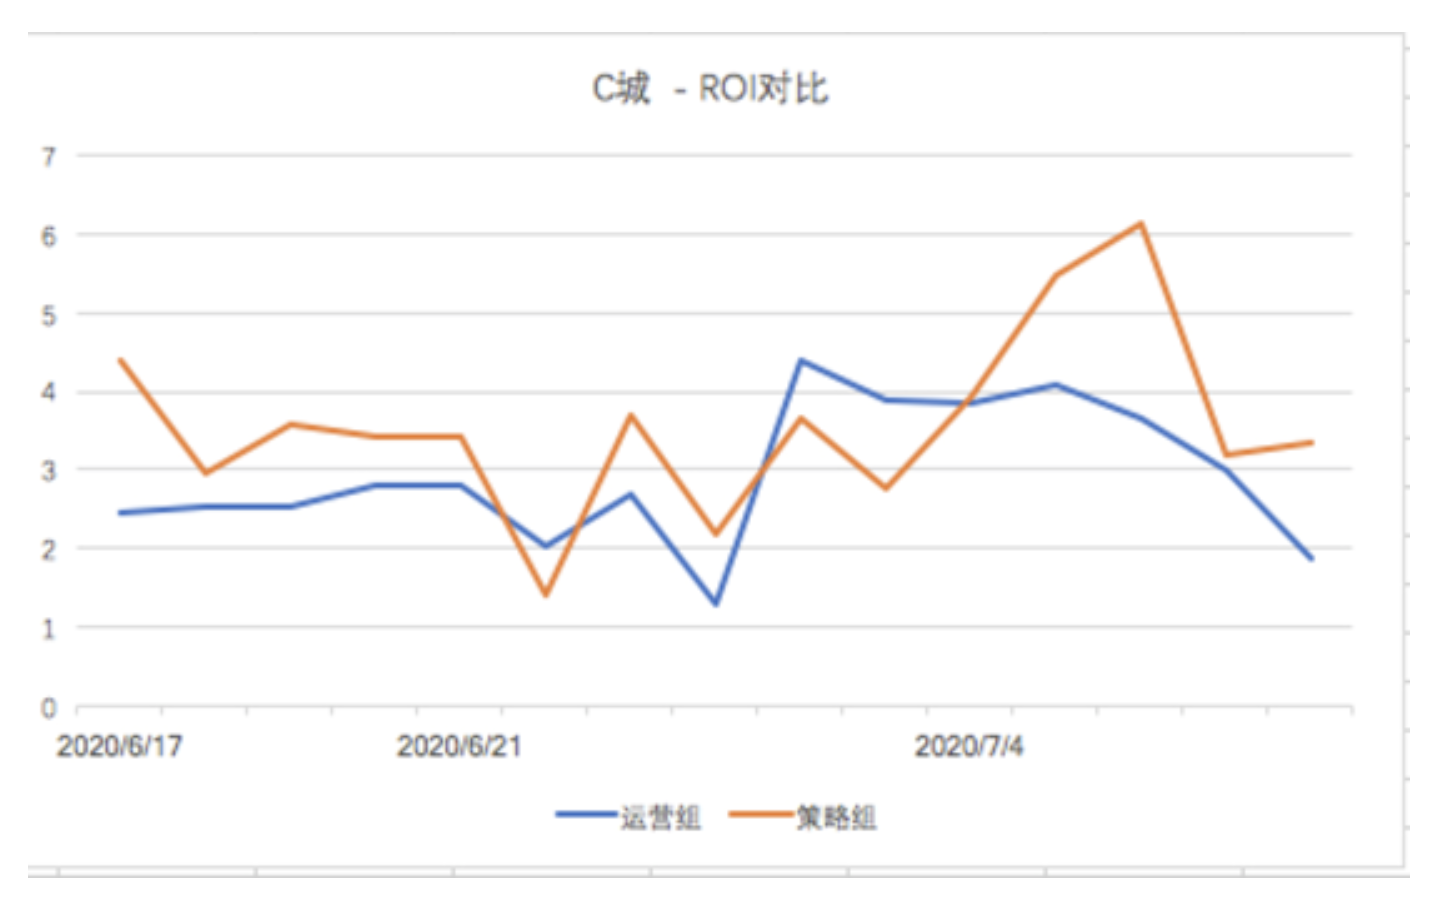
\includegraphics[width=.8\textwidth]{fig/Casual_Inference_In_Didi_19.png}
\end{figure}
\begin{figure}[H]
    \centering
    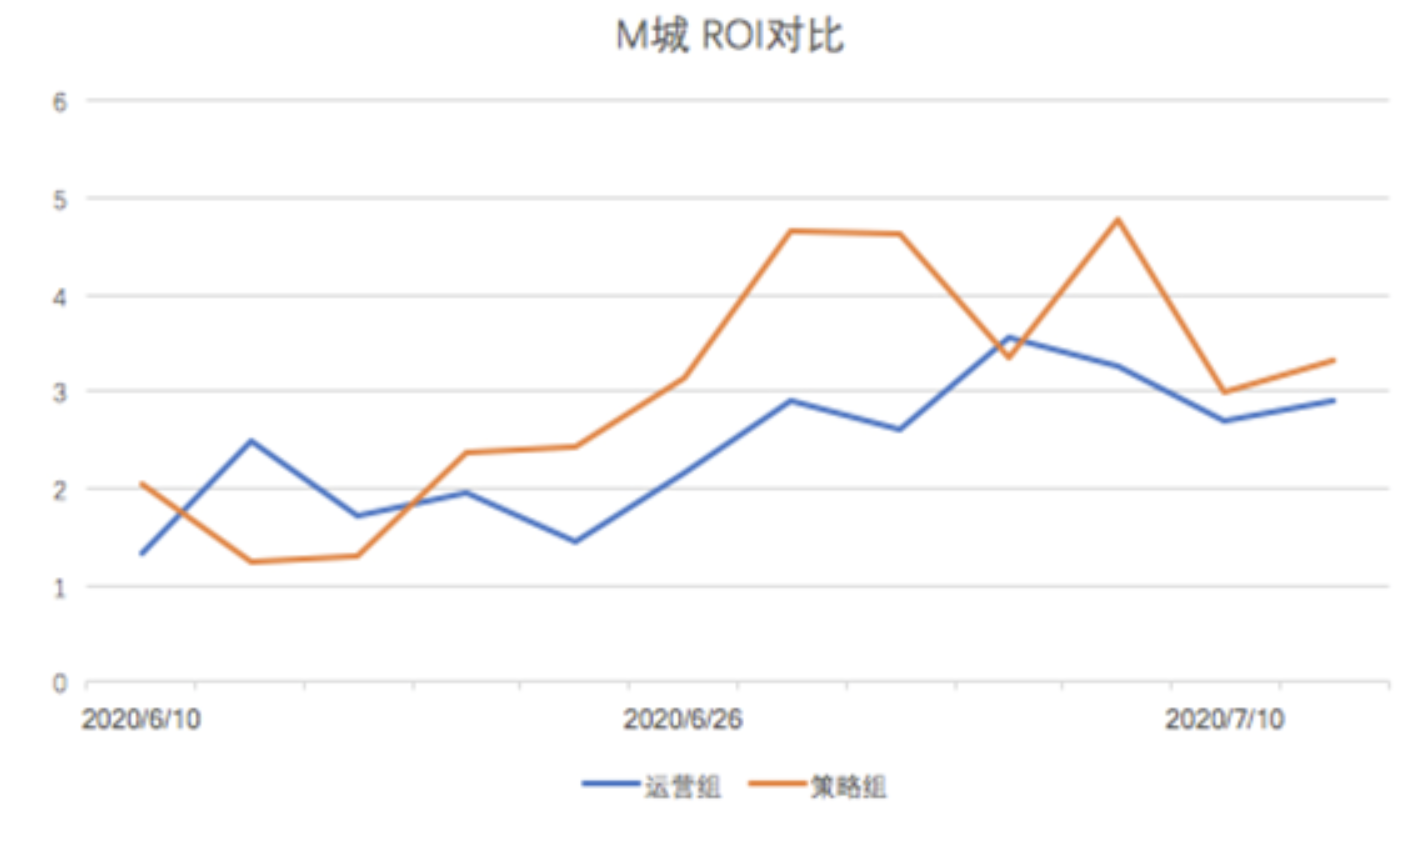
\includegraphics[width=.8\textwidth]{fig/Casual_Inference_In_Didi_20.png}
\end{figure}
\begin{figure}[H]
    \centering
    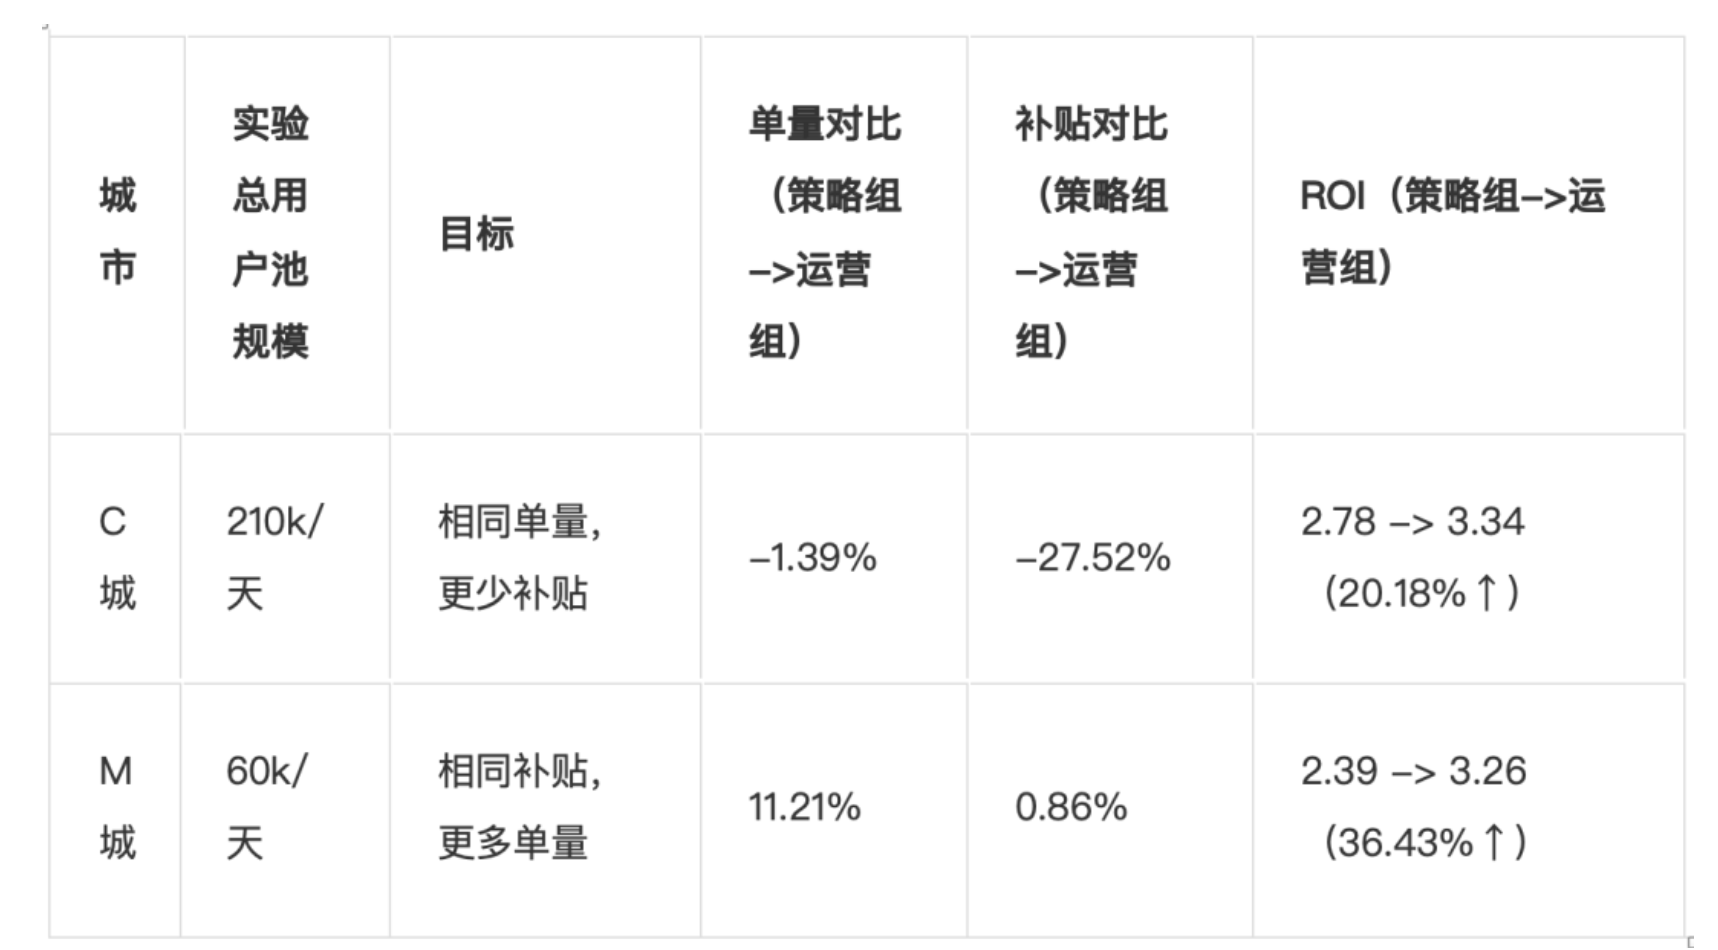
\includegraphics[width=.8\textwidth]{fig/Casual_Inference_In_Didi_21.png}
\end{figure}

可以看出,模型干预策略相比线上baseline,各项指标均有显著优化。在目标【相同单量,更少补贴】下,它确实以单量的略微下降换来了补贴的大幅下降。而在目标【相同补贴,更多单量】下,我们补贴相差无几的同时,单量得到了大幅的提升。

\subsection{未来规划}
我们在20年下半年的规划主要有4个方向:
\begin{itemize}
\setlength{\itemsep}{0pt}
\setlength{\parsep}{0pt}
\setlength{\parskip}{0pt}
    \item 如架构图中所说,我们会把离线的决策模块部分推至线上并引入更多的实时特征和接入更多的发券场景(首页天降红包,进店未下单等等),并将其直接包装为一个简单可解释的运营工具,使其能够提高Local运营效率的同时,解放运营在活动配置上消耗的时间和心力。

    \item 在增量预估模块,我们会持续迭代优化模型。在尝试引入更多维度,信息更丰富的特征的同时,与深度学习模型融合,提高模型精度。

    \item 在分配决策模块,我们会优化整数规划的求解速度并调研和尝试在这个方向上与强化学习理论结合的可能性。

    \item 当前框架下的算法策略几乎只是针对每一次活动希望求得全局的最优化。而在实际运营中,一个健康的补贴生态一定是去优化用户在其整个生命周期的收益的,所以对用户长期价值(LTV)的建模也是个值得规划和探索的方向。
\end{itemize}

\subsection{Q\&A}
\subsubsection{如何正确理解线上的业务指标ROI?}
在解决补贴问题时,时常会困惑如何能合理地解释策略干预的结果,尤其是在与前线运营同学交流的时候。ROI固然是正确且合理的指标,但是我们可以设想这样一个场景,客单价为100,空白组GMV为1000,补贴为0,策略组发放了一个抵扣面额为10的券,最终核销了2张,GMV为1200,补贴为20。那么通过ROI计算公式可得,策略组ROI为200/20=10。与此同时,运营同学发放了一个抵扣面额为20的券,最终核销了10张,GMV为1800,补贴为200,那么运营组的ROI就是800/200=4。从钱效角度出发,当然是策略组干预策略更优秀,但是对于运营同学而言,这次活动确实是他们的策略带来了更多的GMV和单量。
\begin{figure}[H]
    \centering
    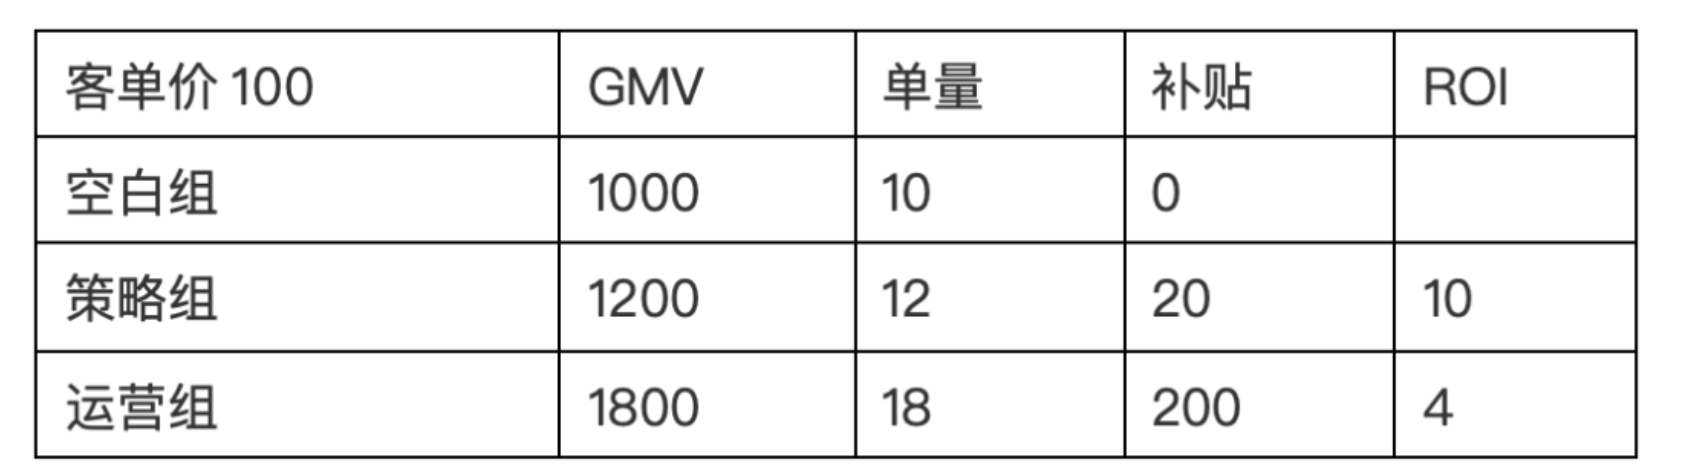
\includegraphics[width=.8\textwidth]{fig/Casual_Inference_In_Didi_22.png}
\end{figure}
而且,运营同学会自然想到的一个原因是因为策略组使用的券种抵扣额度更低,所以ROI会更高,而一旦有了这样的思路,整个过程就不可避免的走向了设计更为复杂且需要运营侧策略侧高度配合的实验。这与我们想高效低廉的解决这个问题就完全背道而驰了。

因此,我们在这个问题上最后的结论是,ROI是一个非常优秀的业务指标,但为了保证策略的可解释性,它不能作为唯一指标。我们锚定了运营同学更为关注的直接指标【规模:GMV,单量】【成本:补贴】,并通过加入约束条件和人工干预的手段,使其中一个维度与运营组策略对齐的同时,观察另一维度指标的提升,也既前面提到了两个大的目标方向【相同单量,更少补贴】和【相同补贴,更多单量】。也就是说,我们只会在【相同补贴】或者【相同单量/GMV】这样的条件下,才去谈论ROI。也只有在这样的情况下,ROI这个指标的说服力才会显得更加强大。

\subsubsection{如何理解离线指标AUUC?}
AUUC是一个很重要且奇怪的指标。说重要,是因为它几乎是Uplift Model在离线阶段唯一一个直观的,可解释的评估模型优劣的指标。说奇怪,是因为它虽然本质上似乎借鉴了分类模型评价指标AUC的一些思想,但是习惯了AUC的算法工程师们在初次接触的时候一定会被它搞得有点迷糊。

作为在分类模型评估上的标杆,AUC的优秀不用过多赘述。其中最优秀的一点是它的评价结果稳定到可以超越模型和样本本身而成立,只要是分类问题,AUC0.5是随机线,0.6的模型还需要迭代一下找找提升的空间,0.6-0.8是模型上线的标准,而0.9以上的模型就需要考虑一下模型是否过拟合和是否有未知强相关特征参与了模型训练。一法抵万法,我们可以抛开特征,样本和模型构建的细节而直接套用这套准则。

然而这个特点对于AUUC就完全是奢望了。\textbf{通过AUUC的公式可以看出,AUUC最终形成的指标的绝对值大小是取决于样本的大小的}。也就是说,在一套测试样本上,我们的AUUC可能是0到1W,而换了一套样本,这个值可能就变成了0到100W。这使得不同测试样本之间模型的评估变为了不可能。也使得每次模型离线的迭代的前提必须是所有模型都使用同一套测试样本。当我们训练完一个新的模型,跑出一个40万的auuc,我们完全无从得知这个值背后代表着模型精度如何,我们只能拿出旧的模型在同样测试集上跑出auuc然后相互比较。这无疑让整个训练迭代过程变得更痛苦了一点。

我们也尝试了从多个角度去解决这个问题,希望在增量预估模型中建立一套类似auc的标准,但无一例外都没能成功。包括像AUC那样除以曲线的理论最大面积,但是看公式就可以知道,这个理论的最大面积其实就是样本个数的平方而这么一除之后得到的AUUC也失去了比较的价值了。

如图所示,即使不是理论的最大面积而是样本排序最优组合的最大面积,也依然超出了衡量的价值。
\begin{figure}[H]
    \centering
    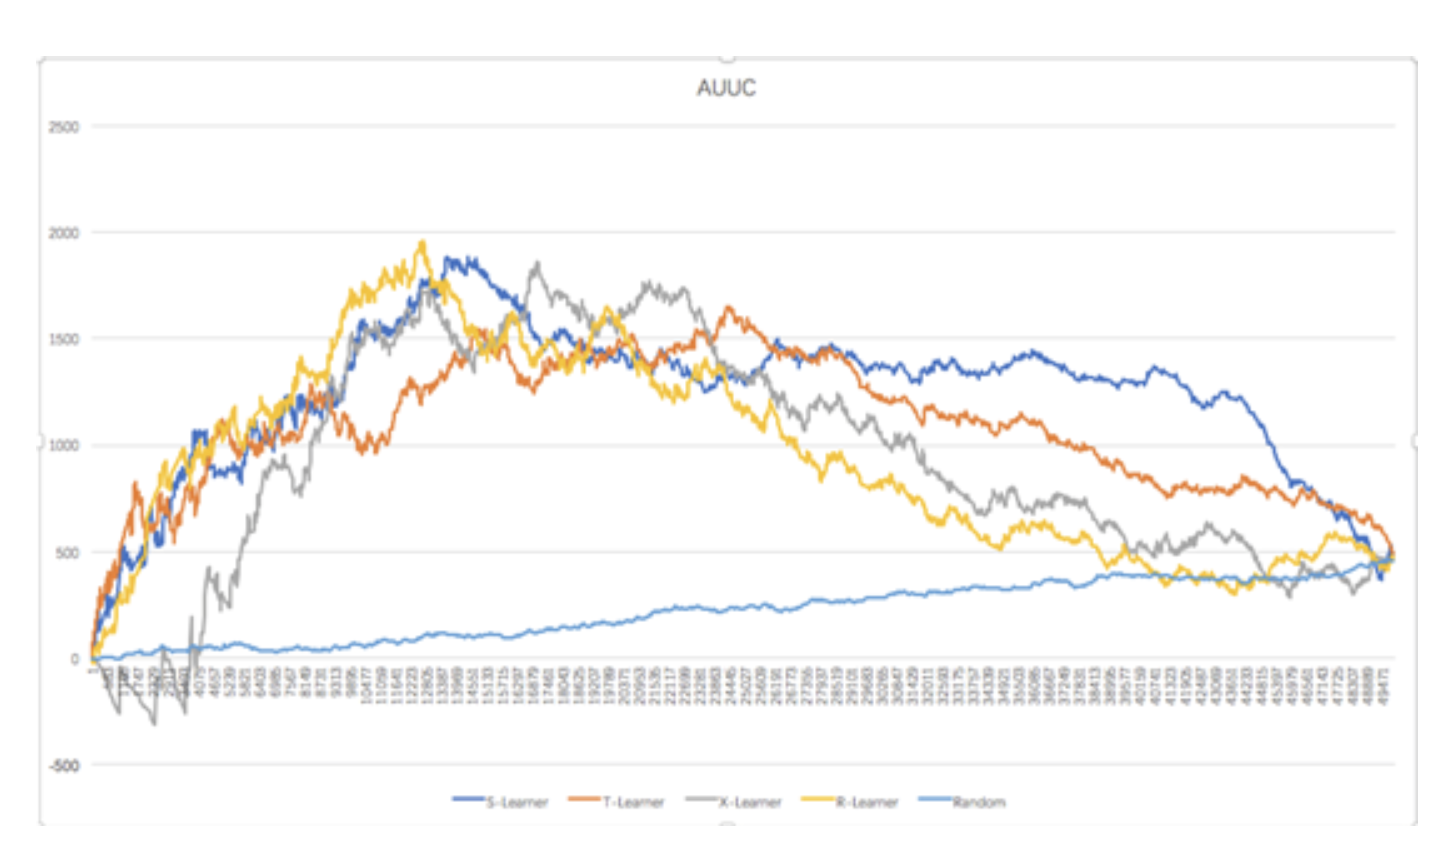
\includegraphics[width=.8\textwidth]{fig/Casual_Inference_In_Didi_23.png}
\end{figure}
\begin{figure}[H]
    \centering
    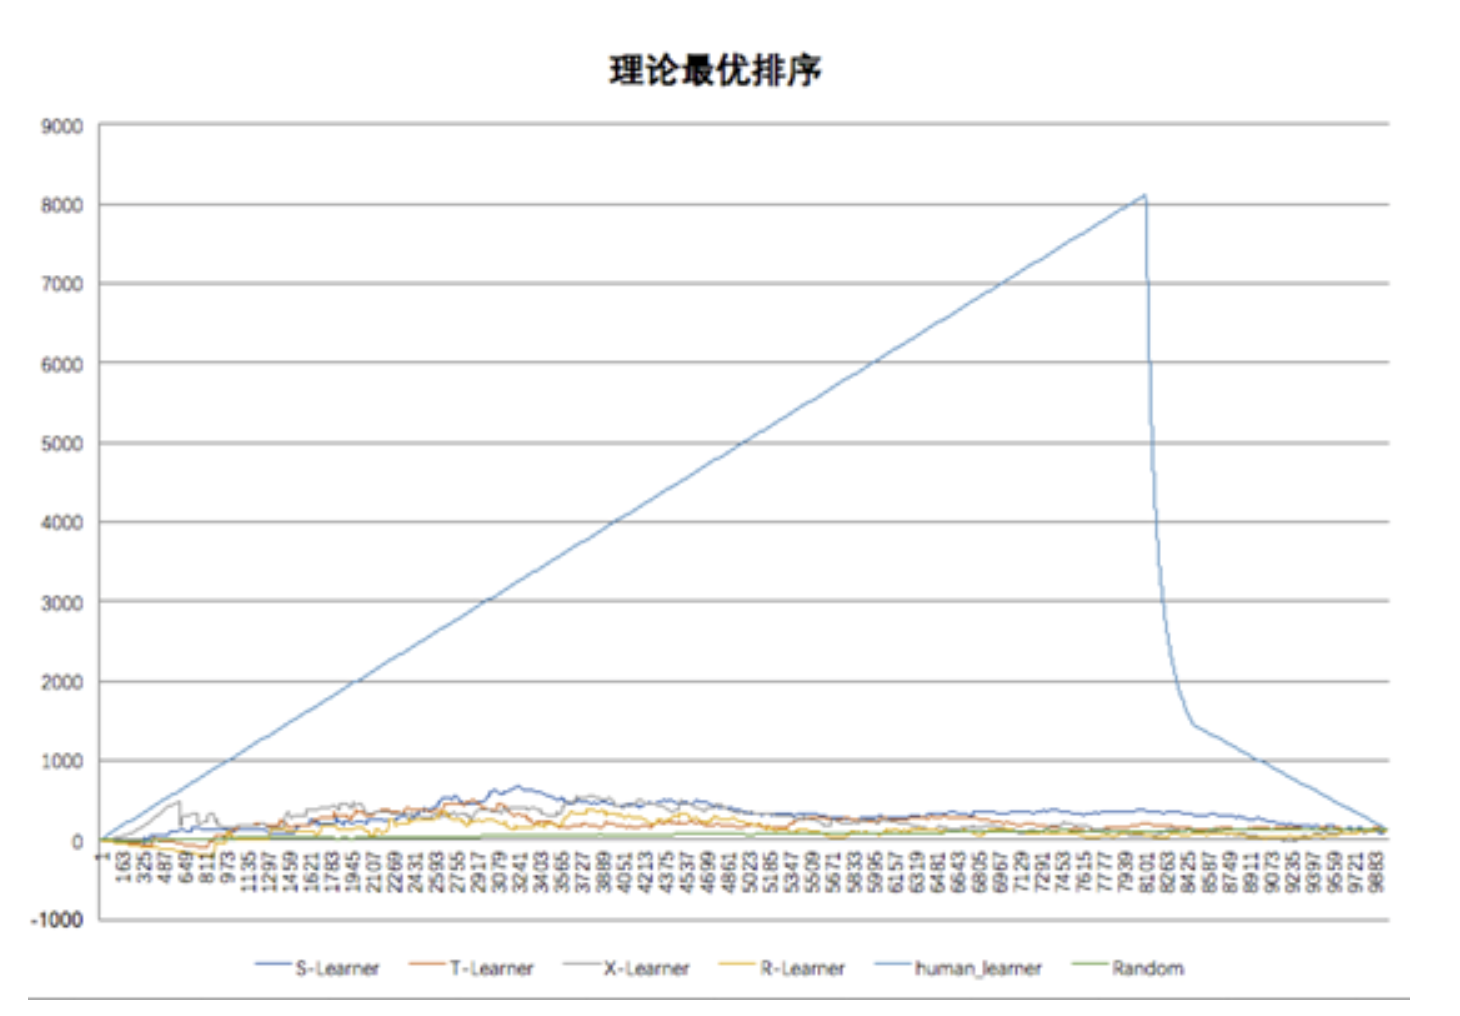
\includegraphics[width=.8\textwidth]{fig/Casual_Inference_In_Didi_24.png}
\end{figure}
我们还尝试过使用AUC的近似计算方法(Pairwise)去近似计算AUUC,得到的结果虽然确保了在0-1区间内的离散性但仍然无法保证在所有情况下,他得出的模型优劣顺序与AUUC本身保持一致。

最后,我们也只能用“补贴问题本身就是与实验批次和样本强相关的问题”这个理由盖过对这个问题的纠结。但能否在增量预估模型中建立一套类似auc的标准,我们仍然认为这个问题是值得投入一点心力去探索的方向。 

%\printbibliography
\bibliography{../ref}
\bibliographystyle{IEEEtran}
\end{document}